\documentclass[handout]{beamer-control}
\begin{document}

\ifonlylectureT{

\begin{frame}[plain]
\centerline{\includegraphics{au-logo}}
\maketitle
\end{frame}

\begin{frame}[plain]
\frametitle{List of Topics}
\tableofcontents[sectionstyle=show,subsectionstyle=hide,subsubsectionstyle=hide,part=1]
\tableofcontents[sectionstyle=show,subsectionstyle=hide,subsubsectionstyle=hide,part=2]
\tableofcontents[sectionstyle=show,subsectionstyle=hide,subsubsectionstyle=hide,part=3]
\end{frame}

}

\setcounter{framenumber}{0}

\documentclass[10pt]{beamer-control}
\usepackage{beamer-control-singlefile}
\INCLUDEONLY{Welcome}
\begin{document}

\lecture{Welcome}{Welcome}

\begin{frame}[plain]
\def\currCONCEPT{Welcome!}
\def\insertsubsectionnumber{0}
\usebeamertemplate{subsection page}
\end{frame}

\begin{frame}
\frametitle{Welcome to Applied Control Systems}
\framesubtitle{An applied but rigorous introduction to control systems for mechanical engineers}

\emph{We hope the course will open your mind and teach practical skills!}
\bigskip

\begin{itemize}
\item What are the learning activities?
\item What is the assessment?
\item What are the requirements?
\end{itemize}
\end{frame}

\begin{frame}
\frametitle{What are the learning activities?}
\begin{itemize}
\item Read the textbook (!)
\item Watch the recorded videos
\item Attend the workshop (computer session---theory)
\item Attend the practical (laboratory---practice)
\end{itemize}
\end{frame}


\begin{frame}
\frametitle{What is the assessment?}
\begin{itemize}
\item Formative quizzes
\item Assignments $\times$3 (15\%)
\item Practical workbooks $\times3$ (non-graded pass)
\item Practical project report (25\%)
\item Exam (60\%)
\end{itemize}
\end{frame}

\begin{frame}
\frametitle{What are the requirements?}
\begin{itemize}
\item Matlab
\item Simulink
\item Mobius for assignments, exam
\item Practical attendance, exam attendance
\end{itemize}
\end{frame}

\begin{frame}
\centering
\Large \alert{Introduction to the textbook}
\end{frame}

\begin{frame}
\includegraphics[width=\linewidth]{astrom}
\end{frame}

\begin{frame}
\frametitle{The course material}
\begin{itemize}[<uncover@+->]
\item Textbook: `\emph{Feedback Systems: An Introduction for Scientists and Engineers}' by Åström \& Murray, 2nd edition.
\item The textbook is perfect for our curriculum:
\begin{itemize}
\item 10 week course, omitting some technical sections
\item No assumption of a `signals and systems' background (Laplace Transforms)
\item Rigorous yet practical with many cross-disciplinary examples
\end{itemize}
\end{itemize}
\end{frame}

\begin{frame}
\frametitle{Alongside the textbook}
\begin{itemize}
\item Additional (background?) textbook material
\item Occasional papers/articles from the literature
\item External online videos for alternate viewpoints
\item Example code
\end{itemize}
\end{frame}

\begin{frame}
\frametitle{About these slides}
\begin{itemize}
\item These slides are not intended to be standalone -- rely on the textbook if in doubt
\item The slides will sometimes interpolate, extrapolate, or introduce certain elements out of place
\item You can suggest improvements to the slides here: \url{https://github.com/AUMAG/applied-control-systems}
\end{itemize}
\end{frame}

\begin{frame}
\frametitle{Course modules and topics}
\small

\centerline{%
\begin{tabular}{>{\hangindent=1em\raggedright\arraybackslash}l>{\hangindent=1em\raggedright\arraybackslash}p{5cm}l}
\toprule
Module & Topic & \S \\
\midrule
Dynamical Systems & Introduction and System Modelling & Ch.1,3 \\ 
& Dynamic Behaviour & Ch.4,5 \\ 
& Linear Systems & Ch.6 \\\midrule
Control System Concepts & State Feedback & Ch.7 \\ 
& Transfer Functions& Ch.9 \\ 
& Frequency Domain Analysis& Ch.10 \\\midrule
Control System Design & PID Control& Ch.11 \\ 
& Frequency Domain Design& Ch.12 \\ 
& Robust Performance \& Fundamental Limits& Ch.13,14  \\
\bottomrule
\end{tabular}}
\end{frame}

\FINALE

\end{document}


\MODULE{Dynamical Systems}

\TOPIC{Introduction and System Modelling}

  \documentclass[10pt]{beamer-control}
\usepackage{beamer-control-singlefile}
\INCLUDEONLY{Introduction}
\begin{document}
\CONCEPT{Introduction}

\begin{SUMMARY}
\begin{itemize}
\item What is a Dynamical System?
\item What is Feedback and Feedforward?
\item What is Control?
\item Feedback Properties (or `why control?')
\item Simple Forms of Feedback
\item Broader Concepts of Control
\end{itemize}
\vfill References:
\begin{itemize}
\item \astrom{Chapter 1}
\item \url{https://engineeringmedia.com/map-of-control}
\end{itemize}
\end{SUMMARY}

\begin{frame}
\frametitle{What is a Dynamical System?}

Dynamical systems have variables (or \emph{states}) $\mathbf{x}$ which change over time:
\begin{align}
\dot {x}(t) = f(\mathbf{x},t)
\end{align}
They generally do not exist alone, and include inputs $\mathbf{u}$:
\begin{align}
\dot {x}(t) = f(\mathbf{x},t) + \mathbf{u}(t)
\end{align}
Dynamical systems can be linear or nonlinear, solvable analytically or only numerically.

\bigskip
\emph{\alert{We must understand dynamical systems before control systems.}}
\end{frame}

\begin{frame}{What is Feedback? \AMref{§1.1}}
\includegraphics[width=\linewidth]{figure1.1}
\end{frame}

\begin{frame}{What is Feedforward? \AMref{§1.2}}
\includegraphics[width=\linewidth]{figure1.3}
\end{frame}

\begin{frame}{What is Control? \AMref{§1.3}}
Augmenting a system to change/improve its dynamics:
\begin{itemize}
\item Passive control: adding a passive element (usually trivial)
\item Active control: adding a feedback (or feedforward) loop
\item Generally involves three elements:
\begin{itemize}
\item Sensors (can't control what you don't know)
\item Controller (calculate what to do based on the state)
\item Actuators (effect the desired changed)
\end{itemize}
\end{itemize}
\end{frame}

\begin{frame}
\frametitle{The canonical control block diagram}

\end{frame}

\begin{frame}{Uses of Feedback and Control \AMref{§1.4}}
Control systems are truly multidisciplinary:
\begin{itemize}
\item Power systems (Elec Eng)
\item Process systems (Chem Eng)
\item Aerospace systems (Mech Eng)
\item Infrastructure systems (Civil/Environ Eng)
\item Economics (tariffs!)
\item Biology, Ecology, Climate Change \dots
\end{itemize}
\end{frame}


\begin{frame}
\frametitle{Simple control systems examples}

\begin{itemize}
\item  Cruise control in a car -- controls velocity
\item  Active noise control headphones -- controls sound pressure level
\item  Voltage regulator circuit -- controls voltage
\item  Hydraulic valve circuit -- controls flow rate
\item  Thermostat (house/oven/sous vide) -- controls temperature
\end{itemize}

\end{frame}

\begin{frame}
\frametitle{Feedback Properties \AMref{§1.5}}
\begin{itemize}
\item<only@1> General solution to asking an engineering system to respond to demands
\item<only@2> Robustness to uncertainty
\begin{itemize}
\item Rejection of disturbances
\item Mitigating sources of error
\item Adapting to changing conditions
\end{itemize}
\item<only@3> Design of dynamics
\begin{itemize}
\item Controlling stability (aerospace)
\item Precise control (robotics)
\end{itemize}
\item<only@4> Challenges
\begin{itemize}
\item Stability
\item Coupling
\item Complexity
\end{itemize}
\end{itemize}
\end{frame}



\begin{frame}
\frametitle{Simple Forms of Feedback \AMref{§1.6}}
\framesubtitle{On-Off Control}
\begin{figure}
	
\includegraphics{figure1.14} \\
	\textbf{Figure 1.14}: Input/output characteristics of on-off controllers.
\end{figure}
\vfil
\begin{gather}
u(t) = \operatorfont{sign}(e)\, u_{\mathrm{max}}
\end{gather}
\end{frame}

\begin{frame}
\frametitle{Simple Forms of Feedback \AMref{§1.6}}
\framesubtitle{PID Control}
\begin{figure}
	
\includegraphics{figure1.15} \\
	\textbf{Figure 1.15}: Action of a PID controller.
\end{figure}
\vfil
\begin{gather}
u(t) = k_p e(t) + k_i \int_0^t e(\tau) \mathrm d\tau + k_d \frac{\mathrm d e(t)}{\mathrm d t}
\end{gather}
\end{frame}

\begin{frame}
\frametitle{Combining Feedback with Logic \AMref{§1.7}}
\includegraphics[width=\linewidth]{figure1.16}
\end{frame}

\begin{frame}
\frametitle{Control System Architectures \AMref{§1.8}}
\centering
\includegraphics[width=0.8\linewidth]{figure1.21}
\end{frame}

\begin{frame}
\frametitle{Brian Douglas' Map of Control Theory}
\centering
\includegraphics[width=0.90\linewidth]{Control_Map_ver5_wr}
\end{frame}

\SUMMARYFRAME
\FINALE

\end{document}

  \documentclass[10pt]{beamer-control}
\usepackage{beamer-control-singlefile}
\INCLUDEONLY{Modeling Concepts}
\begin{document}
\CONCEPT{Modeling Concepts}

\begin{SUMMARY}
\begin{itemize}
\item Systems, models
\item Variables, states, `state space'
\item Example of nonlinear model output
\item Example of linear time-invariant model output
\item Standard control equation
\end{itemize}
\vfill References:
\begin{itemize}
\item \astrom{§3.1}
\end{itemize}
\end{SUMMARY}


\begin{frame}{Systems and models}

\includegraphics[width=\linewidth]{figure3.1}

\end{frame}

\begin{frame}
\frametitle{State model --- mass-spring-damper with nonlinear damping}

\vspace*{-5mm}
\begin{align}
m \ddot q + c(\dot q) + kq &= 0 & x &= \Matr{q\\ \dot q}
\end{align}

\centering
\includegraphics[width=0.9\linewidth]{figure3.2}

\end{frame}

\begin{frame}
\frametitle{Input-output models}
\includegraphics[width=\linewidth]{figure3.3}
\end{frame}

\begin{frame}
\frametitle{Linear time-invariant models}
\includegraphics[width=\linewidth]{figure3.4}
\end{frame}

\begin{frame}
\frametitle{Standard nonlinear control equation}
\begin{align}
\Deriv{x}{t} &= f(x,u) & y &= h(x,u)
\end{align}
Recall nonlinear spring example with $x = [q\quad \dot q]\Tr$:
\begin{align}
\Deriv{x}{t} &= \begin{bmatrix}\dot q\\\ddot q\end{bmatrix} = \begin{bmatrix}\dot q\\- c(\dot q)/m - kq/m\end{bmatrix}
\end{align}
If we measure displacement $q$:
\begin{align}
y = h(x,u) &= q
\end{align}
Use these equations to simulate, simplify, analyse\dots

\end{frame}



\SUMMARYFRAME
\FINALE

\end{document}

  \documentclass[10pt]{beamer-control}
\usepackage{beamer-control-singlefile}
\INCLUDEONLY{State Space Models}
\begin{document}
\CONCEPT{State Space Models}

\begin{SUMMARY}
\begin{itemize}
\item Ordinary Differential Equations
\item Difference Equations
\item Simulation and Analysis
\end{itemize}
\vfill References:
\begin{itemize}
\item \astrom{§3.2}
\end{itemize}
\end{SUMMARY}


\begin{frame}
\frametitle{Terminology}
\begin{itemize}
\item What is a state variable?
\item What is an input?
\item What is an output?
\item What is `dynamics'?
\end{itemize}
\end{frame}

\SUBCONCEPT{Ordinary Differential Equations}

\begin{frame}
\frametitle{State space model}
We have already written this down:
\begin{align}
\Deriv{x}{t} &= f(x,u) & y &= h(x,u)
\end{align}
$x$ is the state vector which contains the state variables, e.g.:
\begin{align}
x = \begin{bmatrix} x_1 \\ x_2 \\ \dot x_1 \\ \dot x_2 \end{bmatrix}
\end{align}
In this example, $x$ is the state vector for an order 4 system.
\end{frame}

\begin{frame}
\frametitle{Linear state space model}
We commonly model state space systems as being `linear time invariant' (LTI).
In the previous concept, we wrote:
\begin{align}
\dot x &= \begin{bmatrix}\dot q\\\ddot q\end{bmatrix} = \begin{bmatrix}\dot q\\- c(\dot q)/m - kq/m\end{bmatrix}
\end{align}
Let's now linearise with $c(\dot q) \eqdef c q$:
\begin{align}
\dot x &= \begin{bmatrix}\dot q\\\ddot q\end{bmatrix} = \begin{bmatrix}\dot q\\- cq/m - kq/m\end{bmatrix}
              = \begin{bmatrix}0 & 1\\- c/m & - k/m\end{bmatrix}\begin{bmatrix} q\\\dot q\end{bmatrix} = Ax
\end{align}
\end{frame}

\begin{frame}
\frametitle{Linear state space equations}
\begin{align}
\dot x &= Ax + Bu & y &= Cx + Du
\end{align}
E.g., if we added an input force to the mass-spring-damper:
\begin{align}
m\ddot q + c\dot q + kq = f
\end{align}
The $Ax$ term is the same, and:
\begin{align}
Bu = \begin{bmatrix} 0\\ 1/m\end{bmatrix}\begin{bmatrix} f\end{bmatrix} = \begin{bmatrix} 0\\ f/m\end{bmatrix}
\end{align}
\QUIZ{Å\&M have a different formulation for $x$ -- is either more correct?}
\end{frame}

\begin{frame}
\frametitle{Equations like this are not just for mechanics!}
\begin{center}
\begin{circuitikz}
  \draw
  (0,0) to[sV, l=$v_s$] (0,3)
        to[R, l=$R$] (3,3)
        to[L, l=$L$] (6,3)
        to[C, l=$C$] (6,0)
        -- (0,0);
\end{circuitikz}
\end{center}

\begin{gather}
L\Deriv{i(t)}{t} + Ri(t) + \frac{1}{C}\int^t_0 i(\tau) \dee \tau = v_s(t) \\
L\ddot q + R\dot q + \frac{1}{C} q = v_s \qquad (i(t) = \dot q(t))
\end{gather}

\end{frame}

\begin{frame}
\frametitle{Now Å\&M throw you in the deep end\dots}
General mechanical dynamics:
\begin{align}
\underbrace{M(q)}_{\text{\tiny inertia matrix}}\ddot q + \underbrace{C(q,\dot q)}_{\text{\tiny coriolis, damping}} + \underbrace{K(q)}_{\text{\tiny potential}} = \underbrace{B(q)u}_{\text{\tiny external}}
\end{align}
`Then it can be shown that' for a Segway-style system:
\begin{align}
\begin{bmatrix}
(M + m) & -ml \cos\theta \\
-ml \cos\theta & (J + ml^2)
\end{bmatrix}
\begin{bmatrix}
\ddot{q} \\
\ddot{\theta}
\end{bmatrix}
+
\begin{bmatrix}
c\dot{q} + ml \sin\theta\, \dot{\theta}^2 \\
\gamma \dot{\theta} - mgl \sin\theta
\end{bmatrix}
=
\begin{bmatrix}
F \\
0
\end{bmatrix}
\label{eq:segway}
\end{align}
\end{frame}


\begin{frame}
\frametitle{Banjo music\dots}
Defining some shorthands:
\begin{align}
M_t &= M+m & J_t&=J+ml^2 & c_\theta&=\cos\theta & s_\theta &= \cos\theta
\end{align}
Equation \eqref{segway} becomes:
\begin{align}
\Deriv{}{t}
\begin{pmatrix}
q \\
\theta \\
\dot{q} \\
\dot{\theta}
\end{pmatrix}
=
\begin{pmatrix}
\dot{q} \\
\dot{\theta} \\
\frac{-ml s_\theta \dot{\theta}^2 + mg(ml^2/J_t) s_\theta c_\theta - c \dot{q} - (\gamma/J_t) ml c_\theta \dot{\theta} + u}
{M_t - m(ml^2/J_t) c_\theta^2} \\
\frac{-ml^2 s_\theta c_\theta \dot{\theta}^2 + M_t gl s_\theta - cl c_\theta \dot{q} - \gamma(M_t/m) \dot{\theta} + lc_\theta u}
{J_t (M_t/m) - m(lc_\theta)^2}
\end{pmatrix}
\end{align}
Output equation:
\begin{align}
y = \begin{bmatrix}
q\\\theta
\end{bmatrix}
\end{align}

\end{frame}

\begin{frame}
\frametitle{Small angle approximations}
With $\mu = M_tJ_t - m^2l^2$:
\begin{align}
\Deriv{}{t}
\begin{bmatrix}
q \\
\theta \\
\dot{q} \\
\dot{\theta}
\end{bmatrix}
=
\begin{bmatrix}
0 & 0 & 1 & 0 \\
0 & 0 & 0 & 1 \\
0 & m^2 l^2 g / \mu & -c J_t / \mu & -\gamma l m / \mu \\
0 & M_t m g l / \mu & -c l m / \mu & -\gamma M_t / \mu
\end{bmatrix}
\begin{bmatrix}
q \\
\theta \\
\dot{q} \\
\dot{\theta}
\end{bmatrix}
+
\begin{bmatrix}
0 \\
0 \\
J_t / \mu \\
l m / \mu
\end{bmatrix}
u
\end{align}

Output:
\begin{align}
y = \begin{bmatrix}
1 & 0 & 0 & 0\\
0 & 1 & 0 & 0
\end{bmatrix}
\begin{bmatrix}
q \\
\theta \\
\dot{q} \\
\dot{\theta}
\end{bmatrix}
\end{align}
\end{frame}

\begin{frame}
\frametitle{This looks like lots of maths}
\begin{itemize}
\item It's important you understand the steps
\item Remember this is a control course, not a dynamics course
\end{itemize}
\end{frame}


\SUBCONCEPT{Difference Equations}

\begin{frame}{Continuous time vs discrete time}
Continuous with $t$:
\def\tt{{\color{orange}(t)}}
\def\kk{{\color{NorthTce}[k]}}
\begin{align}
\Deriv{x\tt}{t} &= f(x\tt,u\tt) & y\tt &= h(x\tt,u\tt)
\end{align}
Discrete with $k$:
\begin{align}
x{\color{NorthTce}[k{+}1]} &= f[x\kk,u\kk] & y\kk &= h(x\kk,u\kk)
\end{align}
Time related by time step $h$:
\begin{align}
x\kk &= x(kh) & k &= 1,2,\dots
\end{align}
\end{frame}

\begin{frame}
\frametitle{Discrete state space equations}
Also natural to write:
\begin{align}
x[k+1] &= Ax[k] + Bu[k] & y[k] &= Cx[k] + Du[k]
\end{align}

Comments:
\begin{itemize}
\item
These are easier and more natural to calculate than continuous ODEs, but they are an approximation
\item
For discrete systems, $A$, $B$, \dots, change depending on the time step
\item
You can learn control entirely from the discrete perspective; we want to consider both but are `continuous by default'
\end{itemize}
\end{frame}

\begin{frame}
\frametitle{Discrete PI Controller}
\begin{align}
u(t) &= K_p e(t) + K_i \underbrace{\int_o^t e(\tau) \dee \tau}_{u_i(t)} & \Deriv{u_i(t)}{t} &= e(t) \\
u[k] &= K_p e[k] + K_i u_i[k]
\end{align}
What is $u_i[k]$ ?
\begin{uncoverenv}<2>
\begin{align}
\Deriv{u_i(t)}{t} &\approx \frac{u_i(kh+h)-u_i(kh)}{h} = e(kh) \\
u_i(kh+h) &= u_i(kh) + he(kh) \\
u_i[k+1] &= u_i[k] + he[k]
\end{align}
\end{uncoverenv}
\end{frame}


\SUBCONCEPT{Simulation and Analysis}

\begin{frame}{Simulation --- our mass-spring-damper system again}
\includegraphics[width=\linewidth]{figure3.10}

Differential form:
\begin{align}
x &= \Matr{q\\\dot q} & \dot x & = \begin{bmatrix}\dot q\\- \frac cm\dot q - \frac km q\end{bmatrix}
\end{align}
$\to$ ODE solver (Matlab, Python)
\end{frame}

\begin{frame}
\frametitle{Simulation --- ODE solvers}
\begin{itemize}
\item Many algorithms for numerically solving ODEs
\item Simulink defaults to \texttt{ode45} with a variable time step solver
\item Important to check solver is accurate -- convergence test(s)
\end{itemize}
\includegraphics[width=\linewidth]{figure3.11}
\end{frame}

\begin{frame}
\frametitle{Analysis --- stability}
\begin{itemize}
\item
Simulations are great, but we sometimes want to analyse our ODEs meaningfully
\item
Lyapunov stability analysis:
\end{itemize}
\begin{align}
V(x) &= \frac12kx_1^2 + \frac12mx_2^2 & \hspace{5cm}\\
\Deriv{V(x)}{t} &=
\end{align}
\vfill
\vspace*{1cm}
\begin{itemize}
\item If $\dot V < 0$, the energy of the system is always decreasing, and the system is therefore \dots
\end{itemize}
\vspace*{-1cm}
\end{frame}

\begin{frame}
\frametitle{Analysis --- frequency response}
For a linear time-invariant system such as: (i.e., separable ODE)
\begin{gather}
m\ddot q + c\dot q + k q = u
\end{gather}
We often consider the input/output relationship in terms of sinusoids of given frequency:
\begin{gather}
u(t) = A\sin(\omega t) \\
q(t) = g(\omega)\sin(\omega t + \phi(\omega))
\end{gather}
The frequency response can be derived (see later) or simulated. For nonlinear systems, things get complicated
\end{frame}

\begin{frame}
\frametitle{Analysis --- sketch of a frequency response}
\end{frame}


\SUMMARYFRAME
\FINALE

\end{document}

  \documentclass[10pt]{beamer-control}
\usepackage{beamer-control-singlefile}
\INCLUDEONLY{Modelling Methodology}
\begin{document}
\CONCEPT{Modelling Methodology}

\begin{SUMMARY}
\begin{itemize}
\item Block diagrams
\item Modelling from experiments
\begin{itemize}
\item ITD, FOTD, SOTD models
\item Estimating models from data
\end{itemize}
\item Normalisation and scaling
\end{itemize}
\vfill References:
\begin{itemize}
\item \astrom{§3.3}
\end{itemize}
\end{SUMMARY}



\SUBCONCEPT{Block diagram}

\begin{frame}{The block diagram}
\includegraphics[width=\linewidth]{figure3.15}
\end{frame}

\begin{frame}
\frametitle{Block diagram elements}
\framesubtitle{Refer \AMref{Figure 3.14}}
\begin{itemize}
\item<alert@1> Sources/sinks
\item<alert@2> Summation
\item<alert@3> Gain
\item<alert@4> Function
\item<alert@5> Derivative
\item<alert@6> Integral
\item<alert@7> Saturation
\end{itemize}
\end{frame}

\begin{frame}
\frametitle{Block diagram of a controller}
\begin{align}
\Deriv{x}{t} &= f(x,u) & y &= h(x) & u &= -ky
\end{align}
\vspace*{0pt plus 1 filll}
\null
\end{frame}


\SUBCONCEPT{Modelling from experiments}

\begin{frame}
\frametitle{Integrator with Time Delay (ITD)}
\begin{columns}
\column{0.4\textwidth}
\only<1>{\includegraphics[width=1.3\linewidth]{itd}}%
\only<2>{\includegraphics[width=1.3\linewidth]{itd-at}}%

\column{0.55\textwidth}
\scriptsize
\begin{uncoverenv}<2>
\begin{itemize}
\item Time delay $\TimeDel$ and intercept $-a$: extrapolate from point of maximum slope
\end{itemize}
\end{uncoverenv}
\end{columns}
\end{frame}

\begin{frame}{First Order system with Time Delay (FOTD)}
\begin{columns}
\column{0.4\textwidth}
\only<1>{\includegraphics[width=1.3\linewidth]{fotd}}%
\only<2>{\includegraphics[width=1.3\linewidth]{fotd-LT}}%

\column{0.55\textwidth}
\scriptsize
\begin{uncoverenv}<2>
\begin{itemize}
\item Steady state response $\StaticGain$:\\ $\StaticGain=1$ for zero steady state error
\item Time delay $\TimeDel$ and intercept $-a$: extrapolate from point of maximum slope
\item Time constant $\TimeConst$: from 63\% of steady state value
\end{itemize}
\end{uncoverenv}
\end{columns}
\end{frame}


\begin{frame}{Second Order system with Time Delay (SOTD)}
\begin{columns}
\column{0.4\textwidth}

\includegraphics[width=1.3\linewidth]{sotd-annot}

\column{0.55\textwidth}
\scriptsize
\begin{itemize}
\item Steady state response $\StaticGain$:\\ $\StaticGain=1$ for zero steady state error
\item Peak response $y_p$ at peak time $T_p$
\item Overshoot $(y_p-\StaticGain)/\StaticGain$ [\%]: measure of dynamic error, increases with smaller damping ratio $\zz$
\item Rise time $t_2-t_1$: measure of the `speed'
\item Settling time $T_s$: another measure of the `speed'; $\epsilon$ usually 1\%, 2\%, or 5\%
\end{itemize}
\end{columns}
\end{frame}

\begin{frame}
\frametitle{Second order system relationships ($m\ddot q + c \dot q + kq = f$)}
Natural frequency $\wn$ and damping ratio $\zz$:
\begin{gather}
\wn = \sqrt{\frac{k}{m}} \qquad \zz = \frac{c}{2\sqrt{km}} 
\end{gather}
Damped natural frequency:\footnote{Note that `resonance frequency' is slightly different: $\wres=\wn\sqrt{1-2\zz^2}$ !}
\begin{align}
\wdamp = \wn\sqrt{1-\zz^2}
\end{align}
Estimate damped natural frequency $\wdamp$ with:
\begin{align}
\wdamp \approx \frac{2\pi}{T_2-T_1}
\end{align}
$T_{1,2}$ are times of successive local maxima in the step response.
\end{frame}

\begin{frame}
\frametitle{Estimating damping ratio}

The decay ratio $d$ often used to estimate the damping ratio
\begin{align}
d=\frac{y_2-\StaticGain}{y_1-\StaticGain}
\end{align}
where $y_{1,2}$ are the amplitudes of successive local maxima in the step response.
\bigskip

Estimate damping ratio $\zz$ with:
\begin{align}
  \zz \approx \frac{1}{\sqrt{1+\left(\frac{2\pi}{\ln d}\right)^2}}
\end{align}
\end{frame}

\begin{frame}
\frametitle{Estimating the remaining parameters (if needed)}
\begin{itemize}
\item
$\wn = \wdamp/\sqrt{1-\zz^2} $
\item
$k = F_0/K$ --- Hooke's law
\item
$m$ follows from $\wn$
\item
$c$ follows from $\zz$
\end{itemize}
\end{frame}

\begin{frame}
\frametitle{Example}
\includegraphics[width=\linewidth]{figure3.16}

\end{frame}

\begin{frame}
\frametitle{Example}
\begin{align}
t_2-t_1&\approx \SI{16}{s} & \therefore~ \wdamp &\approx \SI{0.39}{rad/s} \\
K &\approx \SI{0.5}{m},\quad F_0=\SI{20}{N} & \therefore~ k&\approx \SI{40}{N/m} \\
d&=\frac{y_2-\StaticGain}{y_1-\StaticGain}\approx\frac{\SI{0.16}{m}}{\SI{0.02}{m}}=8 & \therefore~ \zz&\approx0.31  \\
\wn &= \wdamp/\sqrt{1-\zz^2} \approx \SI{0.38}{rad/s} & \therefore~ m &= k/\wn^2 = \SI{277}{kg} \\
&& \therefore~c &= 2\zz\sqrt{km} \approx \SI{66}{kg/s}
\end{align}
This is not quite the same as the textbook --- I expect my numbers were poorly estimated :)

\end{frame}


\SUBCONCEPT{Normalisation and Scaling}

\begin{frame}
\frametitle{Normalisation and Scaling}
\begin{itemize}
\item Where possible, normalise your systems
\item This will generalise the results and make it more likely that off-the-shelf control approaches will be valid
\item Some normalisations are rather mathematical\dots (see example in textbook)
\item Scaling of inputs and outputs is more straightforward:
\end{itemize}
\end{frame}

\begin{frame}
\frametitle{Normalisation}


\begin{figure}
  \centering
  \tikzset{%
    block/.style    = {
                        draw,
                        rectangle,
                        minimum height = 3em,
                        minimum width = 4em,
                        node distance=6em
                      },
    input/.style    = {coordinate},
    output/.style   = {coordinate}
  }

  \begin{tikzpicture}[auto, node distance=2cm, >=latex, thick]

    \draw
    node [input, name=R] {R}
    node [block, right of=R]     (G) {$G$}
    node [output,right of=G] (Y) {}
    ;

    \draw[->](R) -- node {$R$}(G);
    \draw[->](G) -- node {$Y$} (Y);

  \end{tikzpicture}
  \bigskip
  \caption{Plant $P = Y/R$.}
\end{figure}


\begin{figure}
  \centering
  \tikzset{%
    block/.style    = {
                        draw,
                        rectangle,
                        minimum height = 3em,
                        minimum width = 4em,
                        node distance=8em
                      },
    input/.style    = {coordinate},
    output/.style   = {coordinate}
  }

  \begin{tikzpicture}[auto, node distance=2cm, >=latex, thick]

    \draw
    node [input, name=R] {R}
    node [block, right of=R] (RR) {$r_{\mathrm{max}}$}
    node [block, right of=RR] (G) {$G$}
    node [block, right of=G] (YY) {$1/y_{\mathrm{max}}$}
    node [output,right of=YY] (Y) {}
    ;

    \draw[->](R) -- node {$\hat R$}(RR);
    \draw[->](RR) -- node {$R$}(G);
    \draw[->](G) -- node {$Y$} (YY);
    \draw[->](YY) -- node {$\hat Y$}(Y);

  \end{tikzpicture}
  \bigskip
  \caption{Plant $\hat P = \hat Y/\hat R$ with normalisation. (Often implicit, no `hats'.)}
\end{figure}

\end{frame}



\SUBCONCEPT{Examples}

\begin{frame}
\frametitle{Important!}
\begin{itemize}
\item Many of these concepts will be very abstract until you try some examples out
\item Please read through \AMref{§3.4 `Examples'} and try to replicate at least one of them in your own style (pen+paper, Matlab, etc.)
\end{itemize}
\end{frame}

\SUMMARYFRAME
\FINALE

\end{document}


\TOPIC{Dynamic Behaviour}

  \documentclass[10pt]{beamer-control}
\usepackage{beamer-control-singlefile}
\INCLUDEONLY{Solving Differential Equations}
\begin{document}
\CONCEPT{Solving Differential Equations}

\begin{SUMMARY}
\begin{itemize}
\item A little more formal treatment of ODEs
\item Different solution types
\end{itemize}
\vfill References:
\begin{itemize}
\item \astrom{§5.1}
\end{itemize}
\end{SUMMARY}



\begin{frame}{Recalling our differential equations}
Recall our ODE:
\begin{align}
\EqStd
\end{align}
Let's be more formal:
\begin{align}
x &= \Matr{x_1\\x_2\\\vdots\\x_n} \in \Reals^n &
u &= \Matr{u_1\\u_2\\\vdots\\u_p} \in \Reals^p &
y &= \Matr{y_1\\y_2\\\vdots\\y_q} \in \Reals^q
\end{align}
Smooth maps:
\begin{align}
f&\colon\Reals^n \times \Reals^p \to \Reals^n &
h&\colon\Reals^n \times \Reals^p \to \Reals^q
\end{align}
\end{frame}

\begin{frame}
\frametitle{Now add control}
When we design a controller, the input $u$ is generally determined by the state:\footnote{Note: I don't like using uppercase here\dots}
\begin{align}
u &= \alpha(x) & \Deriv{x}{t} &= f(x,u) = f(x,\alpha(x)) \coloneq F(x) \label{eq:Fx}
\end{align}
At this point, $\alpha\colon\Reals^n \to \Reals^p$ could be any smooth nonlinear function
\bigskip

If we can solve $\dot x=F(x)$ we know how the system behaves---what types of solution are possible?
\end{frame}

\begin{frame}
\frametitle{Solution types}
\begin{itemize}
\item We are searching for a specific $x(t)$ which satisfies $\dot x(t)=F(x(t))$
\item Usually care about \emph{initial value problems}
\item Usually there is a unique solution for the particular system
\item Usually there are sinusoids and exponential functions :)
\end{itemize}
\end{frame}

\begin{frame}
\frametitle{Example: damped oscillator}
\begin{itemize}
\item This linear system has a unique analytical solution
\item Note that the solution depends on the damping ratio ($0<\zz<1$)
\item D.E.s with non-unique solutions tend to be nonphysical
\item Counterpoint: read about \href{https://en.wikipedia.org/wiki/Norton\%27s_dome}{Norton's Dome}
\end{itemize}
\end{frame}

\begin{frame}
\frametitle{Example: finite escape time}
\begin{align}
\dot x &= x^2 & x(t) &= \frac{1}{1-t}
\end{align}
\begin{itemize}
\item What happens as $t\to1$ ?
\item $x(t)$ has finite escape time
\end{itemize}
\end{frame}

\begin{frame}
\frametitle{Another example (not in the textbook)}
\begin{align}
\dot x &= x \\
x(t)   &= \ee^{t} \\
x(0)   &= \\
x(t)|_{t\to\infty}&=
\end{align}

\vfill
\hrulefill
\vfill

\begin{align}
\dot x &= -x \\
x(t)   &=  \\
x(0)   &= \\
x(t)|_{t\to\infty}&=
\end{align}
\end{frame}


\SUMMARYFRAME
\FINALE

\end{document}

  \documentclass[10pt]{beamer-control}
\usepackage{beamer-control-singlefile}
\INCLUDEONLY{Qualitative Analysis}
\begin{document}
\CONCEPT{Qualitative Analysis}

\begin{SUMMARY}
\begin{itemize}
\item Vector fields
\item Phase portraits
\item Equilibrium Points
\item Limit Cycles
\end{itemize}
\vfill References:
\begin{itemize}
\item \astrom{§5.2}
\item {\scriptsize\fullcite{bizyaev2024-rcd}\par}
\item {\scriptsize\fullcite{cheffer2021-amm}\par}
\end{itemize}
\end{SUMMARY}



\SUBCONCEPT{Vector fields and Phase portraits}

\begin{frame}
\frametitle{ODE vector field}
Consider the ODE:
\begin{align}
\Deriv{x}{t} = F(x)
\end{align}
\begin{itemize}
\item At every $x$, $F(x)$ defines the `rate of change' of the system
\item We can \emph{plot} this rate of change as a function over state space
\item For a system with two state variables, this is planar plot with a 2D vector defined at all points on the plane
\item This plot is known as a \emph{vector field plot}, or \emph{quiver} plot (\texttt{quiver()} in Matlab)
\end{itemize}
\end{frame}

\begin{frame}
\frametitle{ODE vector field plot}
\framesubtitle{Note the positions of zero vector}
\includegraphics[width=\linewidth]{figure5.3a}
\end{frame}

\begin{frame}
\frametitle{Phase portrait}
\begin{itemize}
\item The vector field is best at highlighting stationary points
\item You can infer but can't directly visualise trajectories
\item Enter the `phase portrait' --- a superimposed collection of trajectories
\item Where the trajectories cluster and converge tells us important properties of the system
\item Note that trajectories don't tell us rate of change
\end{itemize}
\end{frame}

\begin{frame}
\frametitle{Phase portrait plot}
\includegraphics[width=\linewidth]{figure5.3b}

\end{frame}

\SUBCONCEPT{Equilibrium Points and Limit Cycles}

\begin{frame}{Equilibrium point}
For dynamical system $\Deriv{x}{t} = F(x)$, an equilibrium point $x_e$ is:
\begin{align}
\left.\Deriv{x}{t}\right|_{x=x_e} &= F(x_e) = 0
\end{align}
Qualitatively:
\vspace{3cm}
\end{frame}

\begin{frame}
\frametitle{Inverted pendulum equilibria}
This is a second order system with state vector
\begin{gather}
x = \Matr{x_1\\x_2} = \Matr{\theta\\\dot\theta}
\end{gather}
After normalising away constants:
\begin{gather}
\Deriv{x}{t} = \Matr{\dot x_1\\\dot x_2} = \Matr{\dot\theta\\\ddot\theta} = \Matr{\dot\theta\\\sin\theta-c\dot\theta+{\color{red}u\cos\theta}}
\end{gather}
When is $\Deriv{x}{t} = \Matr{0\\0}$ ?

\end{frame}

\begin{frame}
\frametitle{Inverted pendulum equilibria}
\includegraphics[width=\linewidth]{figure5.4}

\end{frame}

\begin{frame}
\frametitle{Limit cycles}
\framesubtitle{Example of an electronic oscillator}
\includegraphics[width=\linewidth]{figure5.5}

\end{frame}

\begin{frame}
\frametitle{Physical system with limit cycle}
\framesubtitle{\minicite{cheffer2021-amm}}

\includegraphics[width=\linewidth]{cheffer2021-fig1}

\end{frame}

\begin{frame}
\frametitle{Physical system with limit cycle}
\framesubtitle{\minicite{cheffer2021-amm}}

\includegraphics[width=0.45\linewidth]{cheffer2021-fig4}\hfil\includegraphics[width=0.45\linewidth]{cheffer2021-fig4}


\end{frame}

\begin{frame}
\frametitle{More complex dynamics example}
\framesubtitle{\minicite{bizyaev2024-rcd}}

\includegraphics[width=\linewidth]{bizyaev2024-fig1}

\end{frame}

\begin{frame}
\frametitle{More complex dynamics example}
\framesubtitle{\minicite{bizyaev2024-rcd}}

\includegraphics[width=\linewidth]{bizyaev2024-fig10}

\end{frame}


\SUMMARYFRAME
\FINALE

\end{document}

  \documentclass[10pt]{beamer-control}
\usepackage{beamer-control-singlefile}
\INCLUDEONLY{Stability}
\begin{document}
\CONCEPT{Stability}

\begin{SUMMARY}
\begin{itemize}
\item Definitions and examples
\item Stability of linear systems
\item Advanced Stability Analysis
\end{itemize}
\vfill References:
\begin{itemize}
\item \astrom{§5.3}
\end{itemize}
\end{SUMMARY}



\SUBCONCEPT{Definitions and examples}

\begin{frame}{Stability}
The stability of a dynamical system is critically important for control systems
\begin{itemize}
\item Sometimes we have an unstable system and wish to stabilise it
\item Sometimes we have a stable system and have to be careful not to destabilise it
\item We will show much later that stability and performance are inextricably linked
\begin{itemize}
\item Control loops (generally) add stability constraints to a system
\item You can design a sluggish system that will always be stable, but if you want to make it responsive you need to push against stability constraints
\end{itemize}
\end{itemize}
\end{frame}

\begin{frame}
\frametitle{Mathematical stability}
\framesubtitle{Sometimes called \emph{stability in the sense of Lyapunov}}
Define $x(t;a)$ as solution to a D.E. with initial condition $a$
\begin{itemize}
\item I.e., $x(t_0) = a$
\item We need to be specific about this because stability needs to be proven for ranges of initial condition!
\end{itemize}
Formally, stability means:
\begin{align}
\|b - a\| < \delta \;\Rightarrow\; \|x(t; b) - x(t; a)\| < \epsilon \quad \text{for all } t > 0.
\end{align}
\end{frame}

\begin{frame}
\frametitle{Example of neutral stability}
\includegraphics[width=\linewidth]{figure5.7}

\end{frame}

\begin{frame}
\frametitle{Asymptotic stability}
\begin{multline}
\|b - a\| < \delta \;\Rightarrow\; \|x(t; b) - x(t; a)\| < \epsilon \quad \text{for all } t > 0, \\
\text{\bf and} \quad \color{NorthTce} \lim_{t \to \infty} \|x(t; b) - x(t; a)\| = 0.
\end{multline}

\includegraphics[width=\linewidth]{figure5.8}


\end{frame}

\begin{frame}
\frametitle{Instability}
\includegraphics[width=\linewidth]{figure5.9}

\end{frame}

\begin{frame}
\frametitle{Bounded stability}
\begin{itemize}
\item For nonlinear systems, we can have stability in a local region around an equilibrium point, but not stability everywhere
\item Define a `ball' of radius $r$ around point $a$:
\begin{align}
B_r(a) = \{ x: \|x-a\| < r \}
\end{align}
\item if $x\in B_r(a)$ is stable, we have \emph{local stability}
\item For all $r>0$, we have \emph{global stability} 
\item \emph{Global asymptotic stability} is the strongest of the common classical stability notions
\end{itemize}
\end{frame}

\SUBCONCEPT{Stability of linear systems}

\begin{frame}{Stability of linear systems}{Linear systems are our key focus}
Nonlinear vs linear dynamical systems:
\begin{align}
\Deriv{x}{t} &= F(x) & \Deriv{x}{t} &= Ax
\end{align}
where $x\in \Reals^n$ and $A\in\Reals^{n\times n}$ is a square matrix

\end{frame}


\begin{frame}{Stability of linear systems}{Linear systems are our key focus}

The stability of the equilibrium point at the origin is given by 
\begin{align}
\lambda(A) \coloneq \{ s\in\mathbb{C} : \operatorname{det}(sI-A)=0 \}
\end{align}
\alert{These are the eigenvalues of the matrix $A$}
\bigskip

\begin{uncoverenv}<2->
The polynomial $\operatorname{det}(sI-A)$ is the characteristic polynomial and the eigenvalues are its roots
\end{uncoverenv}
\bigskip

\begin{uncoverenv}<3->
Eigenvalues are sometimes called `poles' and generally written, for the $j$-th eigenvalue:
\begin{align}
\lambda_j &= \sigma_j \pm \jj\ww_j
\end{align}
\end{uncoverenv}
\end{frame}

\begin{frame}
\frametitle{Stability of linear systems}
\begin{itemize}
\item Important to note: linear systems always have an equilibrium point at the origin
\item (This means that constant terms are `normalised out')
\item Because the $A$ matrix governs the entire state space, stability of linear systems implies global stability
\item Using classical ODE analytical approaches, we can see the solutions of linear systems expressed in terms of sinusoids and exponentials of their eigenvalue components:
\end{itemize}
\begin{align}
\ee^{\sigma_j t} && \sin\ww_j t && \cos\ww_j t
\end{align}
\end{frame}

\begin{frame}{Linear system stability example}{Mass-spring-damper}

\begin{align}
\dot x &= Ax + Bu & y &= Cx + Du
\end{align}
E.g., assume no input force:
\begin{align}
m\ddot q + c\dot q + kq = 0
\end{align}
\begin{align}
\dot x &= \begin{bmatrix}\dot q\\\ddot q\end{bmatrix} = \begin{bmatrix}\dot q\\- cq/m - kq/m\end{bmatrix} 
              = \begin{bmatrix}0 & 1\\- c/m & - k/m\end{bmatrix}\begin{bmatrix} q\\\dot q\end{bmatrix} = Ax
\end{align}

\end{frame}

\begin{frame}{Linear system stability example}{Mass-spring-damper}


\begin{align}
A &= \Matr{0 & 1\\- c/m & - k/m} = \Matr{0 & 1\\- \bar c & - \bar k} \\
sI-A &= \Matr{s & 0\\0 & s} - \Matr{0 & 1\\- \bar c & - \bar k} = \Matr{s & -1\\ \bar c & s+ \bar k} \\
\det(sI-A) &= (s)(s+ \bar k) - (-1)(\bar c) = s^2 + \bar k s  + \bar c
\end{align}
Therefore $\sigma_{1,2}<0$ and $\ee^{\sigma_{1,2} t}\to 0$ as $t\to\infty$: stability

\end{frame}


\SUBCONCEPT{Advanced Stability Analysis}

\begin{frame}{Stability Analysis via Linear Approximation}
\begin{align}
\Deriv{x}{t} &= \Matr{x_2\\\sin x_1-c x_2} \\
\Deriv{x}{t} &\approx \Matr{x_2\\ x_1-c x_2} = \Matr{0 & 1\\1 & -c}\Matr{x_1\\x_2} \\
\Deriv{z}{t} &= \Matr{z_2\\ -z_1-c z_2} = \Matr{0 & 1\\-1 & -c}\Matr{z_1\\z_2}
\end{align}
\end{frame}

\begin{frame}{Stability Analysis via Linear Approximation}
\includegraphics[width=\linewidth]{figure5.11}
\end{frame}



\begin{frame}{Stability of Limit Cycles}{This approach is quite specific --- we would typically focus on simulation models}
\includegraphics[width=\linewidth]{figure5.13}

\end{frame}


\begin{frame}{Lyapunov Stability Analysis — §5.4}{This section is mainly for the applied mathematicians among us}
\begin{itemize}
\item Lyapunov function $V : \Reals^n \to \Reals$ is an energy-like function to determine the stability of the system
\item In short --- if the `energy' of the system decreases to a minimum, we have found an equilibrium point
\item Lyapunov functions are not unique, but in mechanical engineering using \emph{energy} is often appropriate
\item For multi-dimensional systems, phase portraits of $V$ vs $\dot V$ can be used to illustrate complex dynamics 
\end{itemize} 
\end{frame}

\SUMMARYFRAME
\FINALE

\end{document}

  \documentclass[10pt]{beamer-control}
\usepackage{beamer-control-singlefile}
\INCLUDEONLY{Examples}
\begin{document}
\CONCEPT{Examples}

\begin{SUMMARY}
\begin{itemize}
\item Cruise Control
\item Bicycle Dynamics
\end{itemize}
\vfill References:
\begin{itemize}
\item \astrom{Chapter 4}
\end{itemize}
\end{SUMMARY}



\SUBCONCEPT{Cruise Control}

\begin{frame}{Block diagram}
\vfill

\includegraphics[width=\linewidth,clip,trim=0 65 0 0]{figure4.1}

\end{frame}

\begin{frame}{Modelling}{Free body diagram}
\begin{align}
\sum F &= m\ddot x = m\dot v \\
m\dot v &= uf - F_d
\end{align}
\begin{uncoverenv}<2->
\begin{align}
f &= \alpha_n T(\underbrace{\alpha_n v}_{\omega}) \\
T(\omega) &= T_m \biggl( 1 - \beta\Bigl(\frac{\omega}{\omega_m}-1\Bigr)^2 \biggr)
\end{align}
\end{uncoverenv}
\begin{uncoverenv}<3->
\begin{align}
F_d = F_r + F_a + F_g = \underbrace{mg C_r \operatorname{sgn}(v)}_{\text{friction}} + \underbrace{\tfrac12 \rho C_dA|v|v}_{\text{drag}} + \underbrace{mg\sin\theta}_{\text{gravity}}
\end{align}
\end{uncoverenv}
\end{frame}

\begin{frame}
\frametitle{Torque--speed graph}
\includegraphics[width=\linewidth]{figure4.2}

\end{frame}

\begin{frame}
\frametitle{Force--speed graph}
\centering
\includegraphics[scale=0.85]{pdf/car-fv}

\end{frame}

\begin{frame}
\frametitle{Steady state response --- 100\% throttle}
\includegraphics<1->[width=0.45\linewidth]{pdf/cruise-v0}\hfil
\includegraphics<2>[width=0.45\linewidth]{pdf/cruise-t0}
\end{frame}

\begin{frame}
\frametitle{Steady state response --- varying throttle}
\framesubtitle{Note the nonlinearity!}

\includegraphics[width=0.45\linewidth]{pdf/cruise-u}\hfil
\includegraphics[width=0.45\linewidth]{pdf/cruise-uv}
\end{frame}

\begin{frame}
\frametitle{A kind of phase portrait}
\framesubtitle{A single condition is trivial, as this has 1DOF --- $\therefore$ plot multiple conditions}

\centering
\includegraphics[height=0.9\textheight]{pdf/cruise-phase}

\QUIZ{Is this system stable in the sense of Lyapunov?}
\end{frame}

\begin{frame}{Adding a PI Controller}
\begin{itemize}
\item Too much variability/uncertainty to use an ad hoc lookup
\item Hopefully you are convinced a control system is necessary
\item This style of system is well controlled by a `PI' controller:
\end{itemize}
\begin{align}
u &= k_p(v_r-v)+k_iz & \Deriv{z}{t} = v_r-v
\end{align}
Where $e=v_r-v$ and therefore $z=\int_0^t e(\tau) \dee \tau$
\end{frame}

\begin{frame}
\frametitle{ODE with controller}
To study our `controlled' system, augment the state equation:
\begin{align}
x &= \Matr{v\\z} \\
\Deriv{x}{t} &= \Matr{\dot v\\\dot z} = \Matr{\tfrac1m(uf-F_d)\\v_r-v} = F(x) \\
u &= k_p(v_r-v)+k_iz
\end{align}
We now consider $\Deriv{x}{t}=F(x)$ as before.
\end{frame}

\begin{frame}
\frametitle{Cruise control time response}
\centering
\includegraphics[height=0.8\textheight]{pdf/cruise-step}

\end{frame}

\begin{frame}
\frametitle{Cruise control phase portrait}
\centering
\includegraphics[height=0.8\textheight]{pdf/cruise-portrait}

\end{frame}

\SUBCONCEPT{Bicycle Dynamics}

\begin{frame}{Bicycle model}
\includegraphics[width=\linewidth]{figure4.5}
\end{frame}

\begin{frame}{Bicycle dynamics}
\begin{uncoverenv}<1-2>
\begin{align}
J \Deriv{^2\varphi}{t^2} + \frac{Dv_0k_2}{b} \Deriv{\varphi}{t} + \left(\frac{mv_0^2hk_2}{b}-mgh\right)\varphi
&= \frac{Dv_0k_1}{b} \Deriv{T}{t} + \frac{mv_0^2hk_1}{b} T
\end{align}
\end{uncoverenv}
\begin{uncoverenv}<1>
\includegraphics[width=\linewidth]{figure4.6}
\end{uncoverenv}

\end{frame}


\SUMMARYFRAME
\FINALE

\end{document}


\TOPIC{Linear Systems}

  \documentclass[10pt]{beamer-control}
\usepackage{beamer-control-singlefile}
\INCLUDEONLY{Basic Definitions}
\begin{document}
\CONCEPT{Basic Definitions}

\begin{SUMMARY}
\begin{itemize}
\item Linearity
\item Time invariance
\end{itemize}
\vfill References:
\begin{itemize}
\item \astrom{§6.1}
\end{itemize}
\end{SUMMARY}



\SUBCONCEPT{Linearity}

\begin{frame}
\frametitle{Static gain models}
\begin{itemize}
\item Vary input $r=10\%\dots100\%$ (say)
\item Record steady state output vs control input
\item For linear models, slope will be constant
\item For nonlinear models, non-constant slope
\item E.g., rubber or magnetic spring
\end{itemize}
\end{frame}


\begin{frame}[fragile]

\newcommand{\myfig}[6]{%
\begin{scope}[xshift=#6,
             spring/.style = {decorate,
                              decoration = {aspect         = 0.5,
                                            segment length = #1,
                                            amplitude      = 2mm,
                                            coil}}]

\path (0,0)                            coordinate (g)
      (0,-0.5cm)                       coordinate (topspring)
      (0,#2)                           coordinate (bottomspring)
      (bottomspring) ++(0,-.5cm)       coordinate (pt2)
                      +(0cm,-#3)       coordinate (pt3)
                      +(1.25cm,-#3)    coordinate (#5 pt3);

 \node [platform,
        anchor = south] at (g)  {};
 \draw [very thick]    (-1,0)         -- (1,0);
 \draw                (topspring)     -- (g)
                      (bottomspring)  -- (pt2.north);
 \draw [spring]       (bottomspring)  -- (topspring);
 \draw [] (pt3) circle (#3)
                          node[inner sep = 0,
                               scale     = #4,
                               text      = black]{$m_{#5}$};
% \node[right=1.5*#3] at (pt3) {#5} ;
 \end{scope}
}

\begin{tikzpicture}[thick,
                    every node/.style = {draw      = none,
                                         inner sep = 0pt,
                                         outer sep = 0pt},
                    platform/.style   = {fill,
                                         pattern = north east lines,
                                         minimum width  = 2cm,
                                         minimum height  =0.3cm}]
 \myfig{1mm}{-2cm}{0.20cm}{0.5}{A}{-2cm}
 \myfig{3mm}{-3cm}{0.28cm}{0.8}{B}{ 0cm}
 \myfig{3mm}{-4cm}{0.39cm}{1.1}{C}{ 2cm}

\draw[dashed]  (A pt3)  +(-0.4,0)     --               +(0.4,0)
                        +(-0.4+2,0) -- coordinate (b1) +(0.4+2,0)
               (B pt3)  +(-0.4-2,0) -- coordinate (a2) +(0.4-2,0)
               (C pt3)  +(-0.4-2,0) -- coordinate (b2) +(0.4-2,0) ;

\draw[latex-latex] (A pt3) -- node[right=0.1cm]{} (a2);
\draw[latex-latex] (b1)    -- node[right=0.1cm]{} (b2);

\end{tikzpicture}

\end{frame}


\begin{frame}
\frametitle{Linear vs Affine}

\begin{align}
m\ddot x &= -c\dot x - k (x-l_0) - mg + f
\end{align}
\begin{itemize}
\item What is the spring force for $x = l_0$ ?
\item What is the spring force at equilibrium $x_e$ ?
\item Note that the rate of change is the same regardless of the choice of reference point
\end{itemize}
\begin{align}
\Deriv{(x-l_0)}{t} =
\Deriv{(x-x_e)}{t} =
\Deriv{(x)}{t}
\end{align}
So:
\begin{align}
m\ddot {\tilde{x}} &= -c\dot{\tilde x} - k \tilde{x} + f
\end{align}

\end{frame}

\begin{frame}
\frametitle{Affine state space}
Translating systems to their equilibrium point is often \emph{required} due to the form of the state space equations:
\begin{align}
\Deriv{x}{t} = \Matr{\dot x\\\ddot x} = Ax + Bu = \Matr{0 & 1\\ -\frac km & -\frac cm } \Matr{x \\ \dot x} + Bu
\end{align}
Note that there is no constant term!\footnote{Let's just say we \emph{could} include it through  $Bu$  but it's not a good idea.}
\end{frame}

\begin{frame}
\frametitle{Linearity of solutions}
\begin{itemize}
\item<uncover@1-> Principle of superposition:
\begin{itemize}
\item Solution from scaled input $y(\alpha x_0)=\alpha y(x_0)$
\item Solution from multiple inputs $y(x_1+x_2)=y(x_1)+y(x_2)$
\item Etc.\ for $u$
\end{itemize}
\item<uncover@2-> Therefore we often consider:
\begin{itemize}
\item Solution to the homogeneous (or unforced) system \[\Deriv{x_h}{t}=Ax_h\]
\item Solution to the particular (or forced) system \[\Deriv{x_p}{t}=Ax_p+Bu\]
\item And their combinations --- see textbook Example 6.1
\end{itemize}
\end{itemize}
\end{frame}


\SUBCONCEPT{Time invariance}

\begin{frame}{Timey wimey}
Time invariance is a subtle concept:
\begin{itemize}
\item Of course solutions to $\Deriv{x}{t} = Ax$ are time-dependent
\item What we mean is $y_2(t+a) = y_1 (t)$ if $u_2(t+a) = u_1 (t)$
\end{itemize}
\end{frame}

\begin{frame}
\frametitle{Superposition across time}

\includegraphics[width=\linewidth]{figure6.2}


\end{frame}

\begin{frame}
\frametitle{Introducing dirac $\delta(t)$}

Generalising the summation of discrete steps to an arbitrary input signal waveform:
\begin{align}\label{eq:imp}
u(t) = \int^t_0 \ImpulseInput(t-\tau)u(\tau)\dee\tau
\end{align}
where impulse input $\ImpulseInput(t)=S'(t)$ and $S(t)$ is a step input:
\begin{align}
S(t) &=
\begin{cases}
0 & t<0 \\
1 & t\ge 0
\end{cases}
&
\delta(t) &= 
\lim_{\varepsilon\to0}
\begin{cases}
0 & t<0 \\
\tfrac{1}{\varepsilon} & 0<t\le\varepsilon \\
0 & t>\varepsilon
\end{cases}
\end{align}

\end{frame}

\begin{frame}
\frametitle{Output of continuous signal}
We have:
\begin{align}\label{eq:imp}
u(t) = \int^t_0 \ImpulseInput(t-\tau)u(\tau)\dee\tau
\end{align}
This produces output response:
\begin{align}\label{eq:impresp}
y(t) = \int^t_0 \ImpulseResponse(t-\tau)u(\tau)\dee\tau
\end{align}
where impulse response $\ImpulseResponse(t)=\StepResponse'(t)$ and $\StepResponse(t)$ is step response.

\alert{\em The form of \eqref{impresp} is important for the following concepts.}

\end{frame}

\begin{frame}
\frametitle{LTI systems}
\begin{itemize}
\item When is a system not time invariant? Consider, e.g.:
\begin{itemize}
\item a rubber with stiffness that changes with temperature
\item non-Newtonian material with velocity-dependent damping
\item a rocket with fuel mass that burns away over time
\end{itemize}
\item All of classical control theory assumes we have linear, time-invariant (LTI) systems
\item These are generally \emph{good approximations} for most engineering systems
\item Errors due to these assumptions are often handled gracefully by the control system
\item Adaptive and/or nonlinear control is needed for more complex systems
\end{itemize}
\end{frame}

\SUMMARYFRAME
\FINALE

\end{document}

  \documentclass[10pt]{beamer-control}
\usepackage{beamer-control-singlefile}
\INCLUDEONLY{The Matrix Exponential}
\begin{document}
\CONCEPT{The Matrix Exponential}

\begin{SUMMARY}
\begin{itemize}
\item Initial Condition Response
\item Diagonal and Jordan forms
\end{itemize}
\vfill References:
\begin{itemize}
\item \astrom{§6.2}
\end{itemize}
\end{SUMMARY}



\SUBCONCEPT{Initial Condition Response}

\begin{frame}{Generalising system output}
We have shown:
\begin{align}\label{eq:impresp}
y(t) = \int^t_0 \ImpulseResponse(t-\tau)u(\tau)\dee\tau
\end{align}
This form assumes zero initial conditions.

In this concept we:
\begin{itemize}
\item generalise  \eqref{impresp},
\item particularly for nonzero initial conditions.
\end{itemize}
\end{frame}

\begin{frame}
\frametitle{Consider $u=0$}
For unforced system:
\begin{align}
\dot x = A x
\end{align}
For scalar $A=a$, the solution is (naturally)
\begin{align}
x(t) = \ee^{at}x(0)
\end{align}
But note that $a$ could be complex!
\end{frame}

\begin{frame}
\frametitle{For multiple states}

For matrix $A$, we define solution
\begin{align}
x(t) = \ee^{At} x(0)
\end{align}
where $\ee^{At}$ is the \alert{matrix exponential}.
\bigskip

\begin{uncoverenv}<2>
Define $\ee^{At}$ using Taylor series:
\begin{align}
\ee^{At} = I + At + \tfrac12 A^2t^2 + \tfrac{1}{3!}A^3t^3 + \cdots = \sum_{k=0}^{\infty} \tfrac{1}{k!}A^kt^k
\end{align}
As expected: $\Deriv{}{t} \ee^{At} = A \ee^{At}$
\end{uncoverenv}
\end{frame}

\begin{frame}
\frametitle{Linearity of solutions}
Example two-state system:
\begin{align}
x(t) = \Matr{x_1\\x_2} = \ee^{At}\Matr{x_1(0)\\x_2(0)}
\end{align}
\begin{uncoverenv}<2->
Find solutions:
\begin{align}
x_{h1}(t) &= \ee^{At}\Matr{x_{1,0}\\0} &
x_{h2}(t) &= \ee^{At}\Matr{0\\x_{2,0}} 
\end{align}
\end{uncoverenv}
\begin{uncoverenv}<3->
For arbitrary initial condition:
\begin{align}
\ee^{At}\Matr{\alpha x_{1,0}\\\beta x_{2,0}} = \ee^{At}\Matr{\alpha x_{1,0}\\0} + \ee^{At}\Matr{0\\\beta x_{2,0}} = \alpha x_{h1}(t) + \beta x_{h2}(t)
\end{align}
\end{uncoverenv}
\end{frame}

\begin{frame}
\frametitle{Oscillator examples}
For undamped oscillator (mass-spring):
\begin{align}
\ddot q + \ww_0^2 q  = u
\end{align}
Dynamics are normalised using $x_1=q$, $x_2 = \dot q/\ww_0$:
\begin{align}
A &= \Matr{0 & \ww_0\\ -\ww_0 & 0} & \ee^{At} &= \Matr{ \cos \ww_0 t & \sin \ww_0 t \\ -\sin \ww_0 t & \cos \ww_0 t}
\end{align}
Therefore:
\begin{align}
x(t) = \ee^{At} x(0) = \Matr{ \cos \ww_0 t & \sin \ww_0 t \\ -\sin \ww_0 t & \cos \ww_0 t} \Matr{x_1(0)\\ x_2(0)}
\end{align}
\end{frame}

\begin{frame}
\frametitle{Oscillator examples}
For damped oscillator (mass-spring-damper):
\begin{align}
\ddot q + 2 \zz \ww_0 \dot q + \ww_0^2 q  = u
\end{align}
Skipping to the solution:
\begin{align}
x(t) = \ee^{At} x(0) = \ee^{-\zz\ww_0 t} \Matr{ \cos \ww_d t & \sin \ww_d t \\ -\sin \ww_d t & \cos \ww_d t} \Matr{x_1(0)\\ x_2(0)}
\end{align}
where $\wdamp = \ww_0 \sqrt{1-\zz^2}$ (damped natural frequency)
\end{frame}



\SUBCONCEPT{Diagonal and Jordan forms}

\begin{frame}
\frametitle{Diagonal forms}
In the undamped example, $A = \left[\begin{smallmatrix} 0 & \ww_0\\ -\ww_0 & 0\end{smallmatrix}\right]$ and we saw the solution was a linear combination of components.

\bigskip
For larger matrices, can generalise to \alert{diagonal form}:\footnote{\alert{This is the standard convention, opposite the textbook!}}
\begin{align}
\Deriv{x}{t} &= Ax & x &= Tz & \Deriv{z}{t} &= T^{-1}ATz = Jz
\end{align}
(Transformed states $z$ are non-physical)

\end{frame}

\begin{frame}[fragile]
\frametitle{Diagonal $A$ matrix}
Find in Matlab with:
\begin{lstlisting}[style=Matlab-editor]
[T,J] = jordan(A)
\end{lstlisting}
For $A = \left[\begin{smallmatrix} 0 & \ww_0\\ -\ww_0 & 0\end{smallmatrix}\right]$:
\begin{align}
T &= \Matr{ \ii & -\ii \\ 1 & 1  } & J &= T^{-1}AT = \Matr{ -\ww_0 \ii & 0 \\ 0 & \ww_0 \ii}
\end{align}
We can now see intuitively that the solutions will be of the form $\ee^{\ii \ww_0 t}$ which are sinusoids.
\end{frame}

\begin{frame}
\frametitle{Generalised diagonal matrix}
Recall solutions are in the form
\begin{align}
\ee^{At} = I + At + \tfrac12 A^2t^2 + \tfrac{1}{3!}A^3t^3 + \cdots = \sum_{k=0}^{\infty} \tfrac{1}{k!}A^kt^k
\end{align}
For diagonal $A$ matrices:
\begin{align}
A &= \Matr{ \lambda_1 &  &  & 0 \\  & \lambda_2 &  &  \\  &  & \ddots &  \\ 0 &  &  & \lambda_n } \,, &
(At)^k &= \Matr{ \lambda_1^kt^k &  &  & 0 \\  & \lambda_2^kt^k &  &  \\  &  & \ddots &  \\ 0 &  &  & \lambda_n^kt^k }
\end{align}
Combining:
\begin{align}\label{eq:diagform}
\ee^{At} = \Matr{ \ee^{\lambda_1 t} &  &  & 0 \\  & \ee^{\lambda_2 t} &  &  \\  &  & \ddots &  \\ 0 &  &  & \ee^{\lambda_n t} }
\end{align}

\end{frame}

\begin{frame}
\frametitle{Jordan form}
\begin{itemize}
\item Diagonal transformations can't get us to \eqref{diagform} if we have repeated eigenvalues ($\lambda_i=\lambda_j$)
\item In this case couple $k$ number of systems together:
\end{itemize}
\begin{align}
J   &= \Matr{ J_1 &  &  & 0 \\  & J_2 &  &  \\  &  & \ddots &  \\ 0 &  &  & J_k } \,, &
J_i &= \Matr{ \lambda_{i,1} & 1 &  & 0 \\  & \lambda_{i,2} & 1 &  \\  &  & \ddots &  \ddots \\ 0 &  &  & \lambda_{i,j} }
\end{align}
\end{frame}

\begin{frame}
\frametitle{Jordan form solution}
\begin{itemize}
\item Any square matrix can be written in Jordan form \AMref{Theorem 6.2}
\item Once in Jordan form, solution comes as:
\end{itemize}
\begin{align}
\ee^{At} = \Matr{ \ee^{J_1 t} &  &  & 0 \\  & \ee^{J_2 t} &  &  \\  &  & \ddots &  \\ 0 &  &  & \ee^{J_k t} }
\end{align}
with $\ee^{J_i t}$ given along subsequent lines \AMref{Eq (6.11)}
\end{frame}

\begin{frame}
\frametitle{The big reveal}
\begin{itemize}
\item All of this maths is to bring us to a fundamental truth which links linear algebra to ordinary differential equations
\item How do we look at an $A$ matrix to determine the properties of the system?
\item Transformations of $A$ bring us to Jordan form, where see all solutions in terms of $\lambda_i$ eigenvalues:
\end{itemize}
\begin{align}
\ee^{\lambda t} = \ee^{(\sigma + \ii \ww)t} = \ee^{\sigma t} ( \cos \ww t + \ii \sin \ww t)
\end{align}
Stability comes from $\sigma$, therefore:
\begin{theorem}
The system $\dot x=Ax$ is asymptotically stable if and only if all eigenvalues of $A$ have a strictly negative
real part and is unstable if any eigenvalue of $A$ has a strictly positive real part.
\end{theorem}
\end{frame}



\SUMMARYFRAME
\FINALE

\end{document}

  \documentclass[10pt]{beamer-control}
\usepackage{beamer-control-singlefile}
\INCLUDEONLY{Input/Output Response}
\begin{document}
\CONCEPT{Input/Output Response}

\begin{SUMMARY}
\begin{itemize}
\item The Convolution Equation
\item Coordinate Invariance
\item Steady-State Response
\item Frequency Response
\end{itemize}
\vfill References:
\begin{itemize}
\item \astrom{§6.3}
\end{itemize}
\end{SUMMARY}



\SUBCONCEPT{The Convolution Equation}

\begin{frame}{Response to an impulse}
For a state space system:
\begin{align}
\dot x &= Ax + Bu & y &= Cx+Du
\end{align}
We have now seen enough to show:
\begin{align}
x(t) &= \ee^{At}x(0) + \int^t_0 \ee^{A(t-\tau)}Bu(\tau) \dee \tau \\
y(t) &= C\ee^{At}x(0) + \int_0^t \ImpulseResponse(t-\tau) u(\tau) \dee \tau \,.
\end{align}
This is the \alert{convolution equation}; it describes
\begin{itemize}
\item what happens when we perturb the initial condition
\item how the system responds to inputs
\end{itemize}
\end{frame}

\begin{frame}
\frametitle{What is the difference?}
\begin{columns}
\column{0.5\linewidth}
\centerline{\bfseries Initial condition}

\column{0.5\linewidth}
\centerline{\bfseries Impulse response}

\end{columns}
\vspace*{0pt plus 1filll}
\end{frame}

\SUBCONCEPT{Coordinate Invariance}

\begin{frame}{Transforming coordinates does not affect system properties}
\begin{align}
\dot x &= Ax + Bu & y &= Cx+Du
\end{align}
Define transformation $z=Tx$: \footnote{Watch out for $x=Tz$ used elsewhere}
\begin{align}
\dot z &= TAx + TBu & y &= Cx+Du \\
       &= TAT^{-1}z + TBu & y &= CT^{-1}z + Du \\
       &\coloneq \tilde A z + \tilde B u & y &\coloneq \tilde C z + Du
\end{align}
Use $\tilde A$ to analyse more convenient/canonical solution, then transform back.
\end{frame}

\begin{frame}
\frametitle{Coupled mass-spring system}
\vspace*{0pt plus 1filll}
\includegraphics[width=\linewidth]{figure6.7}

\end{frame}

\begin{frame}
\frametitle{Coupled dynamics}

Original:
\[
\Deriv{}{t}\Matr{q_1\\q_2\\\dot q_1\\\dot q_2} =
\underbrace{\begin{bmatrix}
0 & 0 & 1 & 0 \\
0 & 0 & 0 & 1 \\
-\frac{2k}{m} & \frac{k}{m} & -\frac{c}{m} & 0 \\
\frac{k}{m} & -\frac{2k}{m} & 0 & -\frac{c}{m}
\end{bmatrix}}_{A}
\Matr{q_1\\q_2\\\dot q_1\\\dot q_2} +
\begin{bmatrix}
0 \\
0 \\
0 \\
\frac{k}{m}
\end{bmatrix}
u
\]
Transformation:
\[
z = T x = \frac{1}{2}
\begin{bmatrix}
1 & 1 & 0 & 0 \\
0 & 0 & 1 & 1 \\
1 & -1 & 0 & 0 \\
0 & 0 & 1 & -1
\end{bmatrix}
x
=
\frac12
\begin{bmatrix}
q_1 + q_2 \\
\dot{q}_1 + \dot{q}_2 \\
q_1 - q_2 \\
\dot{q}_1 - \dot{q}_2
\end{bmatrix}
\]


\end{frame}

\begin{frame}
\frametitle{Coupled dynamics}
Transformed:
\[
\Deriv{z}{t} =
\begin{bmatrix}
0 & 1 & 0 & 0 \\
-\frac{k}{m} & -\frac{c}{m} & 0 & 0 \\
0 & 0 & 0 & 1 \\
0 & 0 & -\frac{3k}{m} & -\frac{c}{m}
\end{bmatrix}
z +
\begin{bmatrix}
0 \\
\frac{k}{2m} \\
0 \\
-\frac{k}{2m}
\end{bmatrix}
u
\]
\begin{align}
\tilde A &= TAT^{-1} =
\begin{bmatrix}
0 & 1 & 0 & 0 \\
-\frac{k}{m} & -\frac{c}{m} & 0 & 0 \\
0 & 0 & 0 & 1 \\
0 & 0 & -\frac{3k}{m} & -\frac{c}{m}
\end{bmatrix}
=
\begin{bmatrix}
\tilde A_1 & 0 \\
0 & \tilde A_2
\end{bmatrix}
\end{align}
\begin{itemize}
\item Confirm $A$, $\tilde A$, $\tilde A_1$, $\tilde A_2$ all have same eigenvalues
\end{itemize}

\end{frame}

\SUBCONCEPT{Steady-State Response}

\begin{frame}
\frametitle{Response}

\begin{tabular}{|p{2cm}|p{2cm}|p{2cm}|p{2cm}|}
\hline
\multicolumn{4}{|c|}{Response}\\
\hline
\multicolumn{2}{|c|}{Initial condition} & \multicolumn{2}{c|}{Forced}\\
\hline
 &  & Transient & Steady state\\
\hline
\end{tabular}
\bigskip

\begin{itemize}
\item
Transient response: from `mismatch' between initial condition and steady state
\item
Steady state: the long term trend
\end{itemize}
\bigskip

Usually steady-state characteristics follow the input (e.g. constant input leads to constant steady state)

\end{frame}

\begin{frame}
\frametitle{Transient vs steady state response}
\includegraphics[width=\linewidth]{figure6.8}
\end{frame}

\begin{frame}
\frametitle{Step response}
\begin{align}
u(t) &= \StepInput(t)\,, & y(t) &= \StepResponse(t) = \underbrace{CA^{-1} \ee^{At} B}_{\text{transient}} + \underbrace{D-CA^{-1}B}_{\text{steady-state}}
\end{align}

\includegraphics[width=\linewidth]{figure6.9}

\end{frame}


\SUBCONCEPT{Frequency Response}

\begin{frame}
\frametitle{Sinusoidal input}

\begin{align}
u(t) &= \ee^{st}, \qquad s=\ii\ww\,,\\
y(t) &= \underbrace{C \ee^{At} \left( x(0)-(sI-A)^{-1}B \right)}_{\text{transient}} + \underbrace{\left(C(sI-A)^{-1}B+D\right)\ee^{st}}_{\text{steady-state}} &
\end{align}
Consider just steady-state:
\begin{align}
y_{ss}(t) &= \left(C(sI-A)^{-1}B+D\right)\ee^{st} \\
        &= G(s) \ee^{st}
\end{align}
For real sinusoidal input,
\begin{align}
  u(t)&=\cos\ww t \,, &  y_{ss}(t)&= M \cos(\ww t + \theta)
\end{align}
where $M$ is gain and $\theta$ is phase:
\begin{align}
M &= |G(\ii w)| \,, & \theta &= \arg G(\ii w)
\end{align}

\end{frame}

\begin{frame}
\frametitle{Frequency response}
\includegraphics[width=\linewidth]{figure6.11}
\end{frame}

\begin{frame}
\frametitle{Frequency response characteristics}
\begin{description}
\item[Zero frequency gain, $\DCgain$] ~\\Gain for constant inputs (i.e., zero frequency): \[\DCgain = \lim_{\ww\to0}|G(\ii\ww)| = -CA^{-1}B+D\]
\item[Bandwidth, $\wb$] ~\\Frequency range above $\sqrt{\frac12}$ of `reference' (zero frequency gain, usually)
\item[Resonance peak $\Mpeak$ and peak frequency $\wres$] ~\\Maximum amplitude of frequency response gain, and corresponding frequency at which this occurs
\end{description}
\end{frame}

\SUMMARYFRAME
\FINALE

\end{document}

  \documentclass[10pt]{beamer-control}
\usepackage{beamer-control-singlefile}
\INCLUDEONLY{Linearisation}
\begin{document}
\CONCEPT{Linearisation}

\begin{SUMMARY}
\begin{itemize}
\item Jacobian Linearisation
\item Feedback Linearisation
\end{itemize}
\vfill References:
\begin{itemize}
\item \astrom{§6.4}
\end{itemize}
\end{SUMMARY}



\SUBCONCEPT{Jacobian Linearisation}

\begin{frame}{Linearisation steps}
We have nonlinear systems but can often model them linearly:
\begin{itemize}
\item Find or define equilibrium point
\item Shift coordinates so $x_e=0$
\item Make small angle approximations (e.g., $\sin\theta\approx\theta$ for $\theta\approx 0$)
\item More generally, use Taylor series expansion at the equilibrium point and truncate
\end{itemize}
\end{frame}

\begin{frame}
\frametitle{Taylor series expansion}
The Taylor series of differentiable function $f$ about point $a$ is:
\begin{align}
f(x) = f(a) + f'(a)(x - a) + \frac{f''(a)}{2!}(x - a)^2 + \cdots
\end{align}

\begin{align}
x^2 = a^2 + 2a(x - a) + (x - a)^2
\end{align}

\begin{align}
\ee^x = \sum_{n=0}^{\infty} \frac{x^n}{n!} = 1 + x + \frac{x^2}{2!} + \frac{x^3}{3!} + \cdots
\end{align}

\begin{align}
\sin(x) = \sum_{n=0}^{\infty} \frac{(-1)^n}{(2n+1)!} x^{2n+1} = x - \frac{x^3}{3!} + \frac{x^5}{5!} - \cdots
\end{align}
\end{frame}

\begin{frame}
\frametitle{Taylor series linearisation}
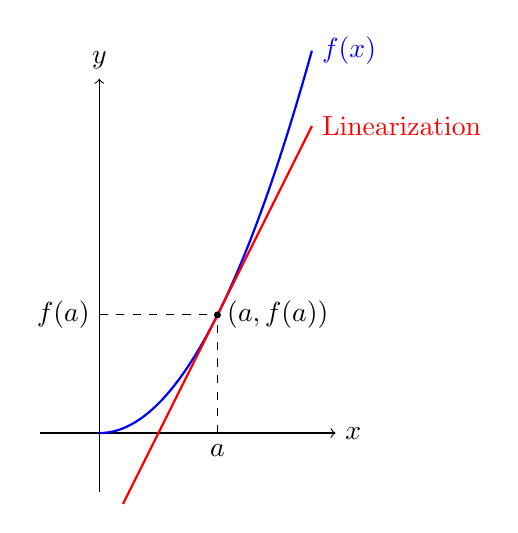
\begin{tikzpicture}[scale=1.5]

  % Axes
  \draw[->] (-0.5,0) -- (2,0) node[right] {$x$};
  \draw[->] (0,-0.5) -- (0,3) node[above] {$y$};

  % Function f(x) = x^2 (example)
  \draw[thick,blue,domain=0:1.8,smooth,samples=100] plot (\x, {\x*\x}) node[right] {$f(x)$};

  % Point a
  \def\a{1}
  \def\fa{\a*\a} % f(a) = a^2
  \def\fpa{2*\a}  % f'(a) = 2a

  % Tangent line at x = a: y = f(a) + f'(a)(x - a)
  \draw[red,thick,domain=0.2:1.8] plot (\x, {\fa + \fpa*(\x - \a)}) node[right] {Linearization};

  % Mark point (a, f(a))
  \filldraw[black] (\a, \fa) circle (0.7pt) node[right] {$(a, f(a))$};

  % Dotted lines to axes
  \draw[dashed] (\a,0) -- (\a,\fa);
  \draw[dashed] (0,\fa) -- (\a,\fa);

  % Labels
  \node at (1, -0.15) {$a$};
  \node[anchor=east] at (0, 1) {$f(a)$};

\end{tikzpicture}

\end{frame}

\begin{frame}
\frametitle{Jacobian linearisation}
The Jacobian $\frac{\partial {f}}{\partial {x}}$ is defined as a matrix of partial derivatives:
\[
{f} : \mathbb{R}^n \to \mathbb{R}^m, \quad
{f}(x_1, x_2, \ldots, x_n) = 
\begin{bmatrix}
f_1(x_1, \ldots, x_n) \\
f_2(x_1, \ldots, x_n) \\
\vdots \\
f_m(x_1, \ldots, x_n)
\end{bmatrix}
\]

\[
\frac{\partial {f}}{\partial {x}} =
\begin{bmatrix}
\frac{\partial f_1}{\partial x_1} & \frac{\partial f_1}{\partial x_2} & \cdots & \frac{\partial f_1}{\partial x_n} \\
\frac{\partial f_2}{\partial x_1} & \frac{\partial f_2}{\partial x_2} & \cdots & \frac{\partial f_2}{\partial x_n} \\
\vdots & \vdots & \ddots & \vdots \\
\frac{\partial f_m}{\partial x_1} & \frac{\partial f_m}{\partial x_2} & \cdots & \frac{\partial f_m}{\partial x_n}
\end{bmatrix}
\]

\end{frame}

\begin{frame}
\frametitle{Jacobian linearisation}
The Jacobian allows a generalised approach. For system:
\begin{align}
\dot x &= f(x,u) & y &= h(x,u)
\end{align}
Define new variables as deviation from equilibrium:
\begin{align}
z &= x - x_e & v &= u - u_e & w&= y-h(x_e,u_e)
\end{align}
Then, linearised system is:
\begin{align}
\dot z &= Az+Bv & w &= Cz + Dv
\end{align}
where
\begin{align}
A &= \left.\PDeriv{f}{x}\right|_{(x_e,u_e)} &
B &= \left.\PDeriv{f}{u}\right|_{(x_e,u_e)} &
C &= \left.\PDeriv{h}{x}\right|_{(x_e,u_e)} &
D &= \left.\PDeriv{h}{u}\right|_{(x_e,u_e)}
\end{align}
\end{frame}

\begin{frame}
\frametitle{Example of Jacobian linearisation}
\centering

\includegraphics[height=0.8\textheight]{example6.12}

\end{frame}

\SUBCONCEPT{Feedback Linearisation}

\begin{frame}{Feedback Linearisation of quadratic term}
E.g., known nonlinearity $x^2$:
\begin{align}
\dot x &= x^2 + u &
u &= -x^2 - kx
\end{align}
The feedback term `cancels' the nonlinearity and adds a `spring' term
\begin{itemize}
\item
What happens if there is an error between the system $x^2$ term and the controller's?
\end{itemize}
\end{frame}

\begin{frame}
\frametitle{Example of feedback linearisation}
\centering

\includegraphics[width=\linewidth]{example6.14}

\end{frame}

\begin{frame}
\frametitle{Block diagram of feedback linearisation}
\centering

\includegraphics[width=\linewidth]{figure6.15}

\end{frame}

\begin{frame}
\frametitle{Dynamic inversion}
Generalised mechanical system with $M(q)$, $C(q,\dot q)$, $B(q)$:
\begin{align}
M(q)\ddot q + C(q,\dot q) = B(q) u \\
u = B(q)^{-1} \left( M(q) \alert{v} + C(q,\dot q) \right)
\end{align}
Resulting dynamics of the system are:
\begin{align}
M(q)\ddot q &= M(q) \alert{v} & \therefore\qquad \ddot q &= v
\end{align}
All dynamics are cancelled, assuming we can model them accurately and the actuators can react appropriately
\end{frame}

\SUMMARYFRAME
\FINALE

\end{document}



\MODULE{Control System Concepts}


\TOPIC{State Feedback}

  \documentclass[10pt]{beamer-control}
\usepackage{beamer-control-singlefile}
\INCLUDEONLY{Reachability}
\begin{document}
\CONCEPT{Reachability}

\begin{SUMMARY}
\begin{itemize}
\item Reachability definition
\item Controllability definition
\item Reachability matrix
\item Reachable canonical form
\end{itemize}
\vfill References:
\begin{itemize}
\item \astrom{§7.1}
\end{itemize}
\end{SUMMARY}



\SUBCONCEPT{Definitions}

\begin{frame}{Reachability}
Consider a system where the state evolution is given by the linear state space equations
\[\frac{\mathrm{d} x}{\mathrm{d} t} = Ax+Bu\]
where $x$ is n-dimensional
\begin{itemize}
\item An important question is, is it possible to find a control signal $u(t)$ such that we can reach any state $x$ in the state space given an initial state $x_0$?
\item The set of states that can be reached by steering the system with control input $u(t)$ for $0\leq t\leq T$ from an initial state $x_0$ is known as the \alert{reachable set}, $\mathcal{R}(x_0,\leq T)$
\end{itemize}
\end{frame}


\begin{frame}{Reachability}
\begin{itemize}
	\item A linear system is \alert{reachable} if,for any initial state $x_0$ and final state $x_f$, there exists a $T>0$ and control $u(t)$ such that $x(0)=x_0$ and $x(T)=x_f$
	\item In other words, the reachable set $\mathcal{R}(x_0,\leq T)$ is our whole state space
	\item This is essentially saying, we can get anywhere in our state space in finite time, no matter where we start!
\end{itemize}

\begin{figure}
	\centering

\includegraphics[width=0.5\linewidth]{figure7.1}
\\
\textbf{Figure 7.1:} The reachable set for a control system.
\end{figure}

\end{frame}	


\begin{frame}{Controllability}
	\begin{itemize}
		\item Reachability is related to a similar property called \alert{controllability}
		\item Rather than asking can we reach any state $x$ given an initial state $x_0$, controllability tackles the problem of controlling our system to a desired position $x_f$ based on a general starting position $x$
		\item These are subtly different but for linear systems, as we study in this course, reachability and controllability are equivalent
	\end{itemize}
\end{frame}


\SUBCONCEPT{Tests for reachability}

\begin{frame}{Reachability matrix}
	\begin{itemize}
		\item Define the reachability matrix
		\[W_r = \begin{bmatrix}
			B & AB & A^2 B & \cdots & A^{n-1}
		\end{bmatrix}\]
		\item A linear system is reachable if and only if the reachability matrix $W_r$ is invertible (or equivalently, full rank)
	\end{itemize}

\end{frame}

\begin{frame}{Example}
	Consider the simplified balance system (which is a model for many examples which the centre of mass is above a pivot point i.e. segway, inverted pendulum)
	\begin{align}
		(M+m)\ddot{p}-ml\cos \theta \ddot{\theta} &= -ml\sin\theta \dot{\theta}^2+F,\\
		(J_ml^2)\ddot{\theta} -ml\cos \theta \ddot{p} &= mgl\sin \theta.
	\end{align}
	Linearising around $(p,0,0,0)$ gives us the state space matrices
	\[ A=\begin{bmatrix}
		0 & 0 & 1 & 0\\
		0 & 0 & 0 & 1\\
		0 & m^2l^2g/\mu & 0 & 0 \\ 0& M_tmgl/\mu & 0 & 0
	\end{bmatrix}, \quad
	B = \begin{bmatrix}
		0 \\ 0 \\ Jt/\mu \\ lm/\mu
	\end{bmatrix}\]
	where $\mu=M_tJ_t-m^2l^2$, $M_t=M+m$, and $J_t=J+ml^2$
\end{frame}

\begin{frame}{Example continued}
The reachability matrix is
\begin{align}
	W_r&= \begin{bmatrix}
		B & AB & A^2 B & A^3B
	\end{bmatrix} \\ 
	W_r &= \begin{bmatrix}
		0 & J_t/\mu & 0 & gl^3m^3/\mu^2 \\ 
		0 & lm/\mu & 0 & gl^2m^2M_t/\mu^2 \\
		J_t/\mu & 0 & gl^3m^3/\mu^2 & 0 \\
		lm/\mu & 0 & g^2l^2m^2M_t/\mu^2 & 0 
	\end{bmatrix}
\end{align}
The determinant of this matrix is $\operatorname{det}(W_r)=-\frac{g^2l^4m^4}{\mu^6}(MJ+mJ+Mml^2)^2\neq 0$ and therefore, the reachability matrix is invertible and so the balance system is reachable!
\end{frame}

\SUBCONCEPT{Reachable canonical form}

\begin{frame}{Coordinate transformation}
\begin{itemize}
	\item Changing the coordinates and writing dynamics in this transformed coordinate system $z=Tx$ often makes calculation more convenient
	\item Reachable canonical form is given by 
	\[\frac{\mathrm{d}z}{\mathrm{d}t} = \begin{bmatrix}
		-a_1 & -a_2 & -a_3 &  \cdots & -a_n	\\
		1 & 0 & & & \\
		& 1& 0 & & & \\
		& & \ddots & \ddots  & \\
		& & & 1 & 0
			\end{bmatrix}z + \begin{bmatrix}
			1 \\ 0 \\ 0 \\ \vdots \\ 0
			\end{bmatrix} u \]
			\[y=\begin{bmatrix}
				b_1 & b_2 & b_3 & \cdots & b_n
			\end{bmatrix}z + du\]
\end{itemize}
\end{frame}

\begin{frame}{Coordinate transformation}
\begin{itemize}
	\item The characteristic polynomial for a system in reachable canonical form is 
	\[\operatorname{det}(sI-A)= s^n+a_1s^{n-1}+\cdots + a_{n-1}s+a_n\]
	\item The reachability matrix in reachable canonical form is
	\[\tilde{W}_r = \begin{bmatrix}
		1 & -a_1 & a_1^2-a_2 & & \\
		0 & 1 & -a_1 & & * \\
		& & \ddots & \ddots & \\
		&  & & 1 & -a_1 \\
		& & & & 1
	\end{bmatrix}\]
	where $*$ are possible nonzero terms
	\item The transformation matrix $T$ can be found by 
	\[T=\tilde{W_r} W_r^{-1}\]
\end{itemize}
\end{frame}


\SUMMARYFRAME
\FINALE

\end{document}

  \documentclass[10pt]{beamer-control}
\usepackage{beamer-control-singlefile}
\INCLUDEONLY{Stabilisation by State Feedback}
\begin{document}
\CONCEPT{Stabilisation by State Feedback}

\begin{SUMMARY}
\begin{itemize}
\item State feedback structure
\item Reachable canonical form
\item Eigenvalue assignment
\end{itemize}
\vfill References:
\begin{itemize}
\item \astrom{§7.2}
\end{itemize}
\end{SUMMARY}



\SUBCONCEPT{State feedback structure}

\begin{frame}{Controller structure}
\begin{itemize}
\item We will assume we have a system with a linear state model that has a single input for control
\item How do we design the dynamics of a system through feedback of the state?
\item The goal of a feedback controller is to control the output state $y$ to a desired state given by the input $r$
\end{itemize}
\begin{figure}
	\centering
	
\includegraphics[width=0.8\linewidth]{figure7.5}
	\\
	\textbf{Figure 7.5:} A feedback control system with state feedback.
\end{figure}
\end{frame}


\begin{frame}{Controller structure}
	\begin{itemize}
		\item Consider a system described by
		\[ \frac{\mathrm{d} x}{\mathrm{d} t}=A x+B u, \quad y=C x+D u\]
		\item A linear control law dependent on the state $x$ and reference input $r$ can be given by 
		\[u = -Kx + k_f r\] 
		giving the closed loop state space representation 
		\[\frac{\mathrm{d} x}{\mathrm{d} t} = (A-BK)x + Bk_f r \]
	\end{itemize}
\end{frame}


\begin{frame}{Controller structure}
	\begin{itemize}
		\item We can therefore determine the characteristic polynomial of the closed loop system from our state space representation
		\item Comparing this to a \textit{desired} characteristic polynomial,
		\[p(s) = s^n + p_1 s^{n-1} + \cdots p_{n-1} s + p_n\] 
		we can design our gains $K$ and $k_f$ to meet performance specifications 
		\item Typically we want a stable equilibrium point, but maybe we care about rise time, settling time, overshoot as well 
	\end{itemize}
\end{frame}

\SUBCONCEPT{State feedback in reachable canonical form}

\begin{frame}{Reachable canonical form}
\begin{itemize}
\item Consider a system in reachable canonical form
\[\frac{\mathrm{d} z}{\mathrm{d} t}=\tilde{A} z+\tilde{B} u=\begin{bmatrix}
	-a_1 & -a_2 & -a_3 & \ldots & -a_n \\
	1 & 0 & & &  \\
	& 1 & 0 & & \\
	& & \ddots & \ddots & \\
	& & & 1 & 0
\end{bmatrix} z+\begin{bmatrix}
	1 \\
	0 \\
	0 \\
	\vdots \\
	0
\end{bmatrix} u\]
\[  y=\tilde{C} z=\begin{bmatrix}
	b_1 & b_2 & \cdots & b_n
\end{bmatrix}z \]
\item From the \alert{Reachability} lecture slides, the open loop system has characteristic polynomial
\[\operatorname{det}(sI-A) = s^n+a_1s^{n-1}+\cdots + a_{n-1}s+a_n\]
\end{itemize}
\end{frame}

\begin{frame}{Reachable canonical form }
	\begin{itemize}
		\item For control law \[u=-\tilde{K}z+k_f r=-\tilde{k}_1z_1-\tilde{k}_1z_1- \cdots - \tilde{k}_nz_n+k_fr,\] the closed loop system is 
		\[  \frac{\mathrm{d} z}{\mathrm{d} t}=\begin{bmatrix}
			-a_1-\tilde{k}_1 & -a_2-\tilde{k}_2 & -a_3-\tilde{k}_3 & \ldots & -a_n-\tilde{k}_n \\
			1 & 0 & & & \\
			& 1 & 0 & & \\
			&  & \ddots & \ddots & \\
			& & & 1 & 0
		\end{bmatrix} z+\begin{bmatrix}
			k_{\mathrm{f}} \\
			0 \\
			0 \\
			\vdots \\
			0
		\end{bmatrix} r  \]
		\[y = \begin{bmatrix}
			b_1 & b_2 & \cdots & b_n
		\end{bmatrix}z\]
		\item The closed loop system has characteristic polynomial
		\begin{align}
		\operatorname{det}(sI-A+BK) &= s^n+\left(a_1+\tilde{k}_1\right) s^{n-1}+\left(a_2+\tilde{k}_2\right) s^{n-2}\\
		&+\cdots+\left(a_{n-1}+\tilde{k}_{n-1}\right) s+a_n+\tilde{k}_n   \end{align}
	\end{itemize}
\end{frame}


\begin{frame}{Reachable canonical form}
\begin{itemize}
	\item Therefore, we find that relating the desired characteristic polynomial to the closed loop characterisic polynomial we have
	\[\tilde{K} = \begin{bmatrix}
		p_1-a_1 & p_2-a_2 & \cdots & p_n-a_n
	\end{bmatrix}\]
	\item Further, to have zero frequency gain equal to unity we have
	\[k_f = \frac{a_n+\tilde{k}_n}{b_n}=\frac{p_n}{b_n}\]
\end{itemize}
\end{frame}



\SUBCONCEPT{Eigenvalue assignment}
\begin{frame}{Design with reachable canonical form}
This process allows us to assign the eigenvalues of the closed loop system to the eigenvalues of a desired system only if the system is reachable
\begin{enumerate}
	\item Given a linear state space model, $A$, $B$, $C$, and $D$, calculate the characteristic polynomial
	\[\operatorname{det}(sI-A) = s^n+a_1s^{n-1}+\cdots + a_{n-1}s+a_n\]
	\item Calculate gains in reachable canonical form  
	by determining  \[W_r = \begin{bmatrix}
		B & AB & A^2 B & \cdots & A^{n-1}
	\end{bmatrix},\quad \tiny{\tilde{W}_r = \begin{bmatrix}
		1 & -a_1 & a_1^2-a_2 & & \\
		0 & 1 & -a_1 & & * \\
		& & \ddots & \ddots & \\
		&  & & 1 & -a_1 \\
		& & & & 1
	\end{bmatrix}}\]
\end{enumerate}
\end{frame}

\begin{frame}{Design with reachable canonical form}
\begin{enumerate}
	\setcounter{enumi}{2}
	\item The feedback gains to give a closed loop system with unity zero frequency gain between $r$ and $y$ and characteristic polynomial
	\[p(s) = s^n+p_1 s^{n-1}+ \cdots p_{n-1}s+p_n\]
	is given by 
	\[K=\tilde{K}T = \begin{bmatrix}
		p_1-a_1 & p_2-a_2 & \cdots & p_n-a_n
	\end{bmatrix} \tilde{W}_r W_r^{-1}\]
	\[k_f = \frac{p_n}{b_n}\]
\end{enumerate}
This method is implemented in Matlab in the functions \textbf{acker} and \textbf{place}
\end{frame}

\begin{frame}{Example}
The predator-prey model is given by 
\[\frac{\mathrm{d}H}{\mathrm{d}t} = (r+u)H\left(1-\frac{H}{k} \right)-\frac{aHL}{c+H}, \quad \frac{\mathrm{d}L}{\mathrm{d}t} = \frac{baHL}{c+H}-dL\]
where the population of an ecosystem can be regulated by controlling the food supply

\begin{figure}
	\centering
	
\includegraphics[width=0.8\linewidth]{figure4.20}
	\\
	\textbf{Figure 4.20:} Simulation results for the uncontrolled predator-prey system ($u=0$).
\end{figure}

\end{frame}


\begin{frame}{Example continued}
Choosing parameters $a=3.2$, $b=0.6$, $c=50$, $d=0.56$, $k=125$,  $r=1.6$, taking the growth rate for hares as the input to the system $u$ (potentially controlled by a food source for the hares), taking the number of lynxes $L$ as the output, and linearising around the equilibrium point we get 
	\[\frac{\mathrm{d}}{\mathrm{d}t}\begin{bmatrix}
		z_1 \\ z_2
	\end{bmatrix} = \begin{bmatrix}
		0.13 & -0.93 \\ 0.57 & 0
	\end{bmatrix} \begin{bmatrix}
		z_1 \\ z_2
	\end{bmatrix}  + \begin{bmatrix}
		17.2 \\ 0
	\end{bmatrix} v\]
	\[w=\begin{bmatrix}
		0& 1
	\end{bmatrix}  \begin{bmatrix}
		z_1 \\ z_2
	\end{bmatrix} \]
where $z_1=H-H_e$, $z_2=L-L_e$, and $v=u$
	
This system is reachable (by showing that the reachability matrix is full rank) and therefore we can assign the eignenvalues using state feedback

\end{frame}

\begin{frame}{Example continued}
	
	Choosing $\lambda=\begin{bmatrix}
		-0.1 & -0.2
	\end{bmatrix}$ as our desired eigenvalues, we may use the eigenvalue assignment approach to get $K=\begin{bmatrix}
		0.025 & -0.052
	\end{bmatrix}$ and $k_f=0.002$ for our gain values
	
	The resulting control law tells us how we should change the food source for the hares as a function of the current number of lynxes and hares to stabilise both populations to their equilibria
\begin{figure}
	\centering
	
\includegraphics[width=0.8\linewidth]{figure7.7}
	\\
	\textbf{Figure 7.7:} Simulation for the controlled predator-prey system.
\end{figure}
\end{frame}


\SUMMARYFRAME
\FINALE

\end{document}

  \documentclass[10pt]{beamer-control}
\usepackage{beamer-control-singlefile}
\INCLUDEONLY{Design Considerations}
\begin{document}
\CONCEPT{Design Considerations}

\begin{SUMMARY}
\begin{itemize}
\item Second-order systems
\item Higher-order systems
\end{itemize}
\vfill References:
\begin{itemize}
\item \astrom{§7.3}
\end{itemize}
\end{SUMMARY}



\SUBCONCEPT{Second-order systems}


\begin{frame}{Design considerations}
\begin{itemize}
\item The location of the eigenvalues of a system may be chosen with appropriate state feedback and these locations are the main design consideration
\item There is a trade-off between closed-loop performance, robustness of the system, and magnitude of control inputs
\item We examine these by studying second-order systems
\end{itemize}
\end{frame}


\begin{frame}{Second-order dynamics}
A general second-order system is given by the differential equation
\[\ddot{q}+2\zeta \omega_0 \dot{q}+\omega_0^2q=k\omega_0^2u, \quad y=q.\]
The state space representation is 
\[\frac{\mathrm{d} x}{\mathrm{d} t}=\begin{bmatrix}
	0 & \omega_0 \\
	-\omega_0 & -2 \zeta \omega_0
\end{bmatrix} x+\begin{bmatrix} 0 \\
k \omega_0 
\end{bmatrix}u, \quad y=\begin{bmatrix}
	1 & 0
\end{bmatrix} x,\]
where $x=\left(q,\tfrac{\dot{q}}{\omega_0}\right)$ is a normalised choice of states.\\
The parameter $\omega_0$ is known as the natural frequency of the system and $\zeta$ is known as the damping ratio.
\end{frame}

\begin{frame}{Second-order dynamics}
The eigenvalues of this general system are 
\[\lambda=-\zeta \omega_0 \pm \omega_0 \sqrt{\zeta^2-1}.\]	
From this we can deduce that the system is stable if $\omega_0>0$ and $\zeta>0$. Also, the eigenvalues are complex if $\zeta<1$ and are real if $\zeta\geq 1$.\\

The parameter $\zeta$ describes systems that are
\begin{itemize}
	\item overdamped if $\zeta>1$ and exhibits exponentially decaying dynamics,
	\item critically damped if $\zeta=1$ and gives similarly decaying dynamics, 
	\item and is underdamped if $0<\zeta < 1$ where the solutions are oscillatory with damped frequency $\omega_d=\omega_0\sqrt{1-\zeta^2}$.
\end{itemize}
\end{frame}

\begin{frame}{Second-order dynamics}
The simple form of second-order systems means we can derive analytical expressions for time and frequency responses.
\begin{figure}
	\centering
	
\includegraphics[width=0.5\linewidth]{figure7.8}
	\\
	\textbf{Figure 7.8:} Step response for a second-order system.
\end{figure}
\begin{figure}
	\centering
	
\includegraphics[width=0.5\linewidth]{figure7.9}
	\\
	\textbf{Figure 7.9:} Frequency response for a second-order system.
\end{figure}
\end{frame}


\begin{frame}{Second-order dynamics}
We can compute properties of the step response analytically as well

\begin{center}
	\begin{tabular}{|c|c|}
	\hline
	Property & Value\\ & \\
	\hline
	Steady-state value & $k$ \\  & \\
	Rise time & $T_r=\frac{e^\frac{\varphi}{\tan \varphi}}{\omega_0}$, where $\varphi=\arccos \zeta$ \\ & \\
	Overshoot & $M_p=e^{\frac{-\pi \zeta}{\sqrt{1-\zeta^2}}}$ \\ & \\
	2\% settling time & $T_s\approx \frac{4}{\zeta \omega_0}$
	\\
	\hline
\end{tabular}
\end{center}
\end{frame}


\SUBCONCEPT{Higher-order systems}

\begin{frame}{Dominant eigenvalues}
\begin{itemize}
\item Systems more complicated than second-order are characterised by the dominant eigenvalues
\item For stable systems, dominant eigenvalues are those that are closest to the imaginary axis as these correspond to the `slowest' response
\item By superposition, the faster dynamics corresponding to eigenvalues further from the imaginary axis will decay much quicker than the dominant terms
\item For eigenvalue assignment of higher-order systems, we therefore must consider how the dominant poles will affect the dynamics in closed-loop
\end{itemize}
\end{frame}


\SUMMARYFRAME
\FINALE

\end{document}

  \documentclass[10pt]{beamer-control}
\usepackage{beamer-control-singlefile}
\INCLUDEONLY{Integral Action}
\begin{document}
\CONCEPT{Integral Action}

\begin{SUMMARY}
\begin{itemize}
\item System augmentation
\item Reachability of the augmented system
\end{itemize}
\vfill References:
\begin{itemize}
\item \astrom{§7.4}
\end{itemize}
\end{SUMMARY}



\SUBCONCEPT{System augmentation}

\begin{frame}{Integral action}
\begin{itemize}
\item When a perfect model is available, state feedback allows systems in closed-loop to track command signals
\item In cases where our model is only approximately accurate, our controller may have non-zero steady-state error
\item When \alert{integral feedback} is introduced, even if we have errors in our model parameters or disturbances to our system, the controller will compensate and result in perfect tracking
\end{itemize}
\end{frame}

\begin{frame}{Integral action}
The idea is to add an additional state to our system that computes the integral of the error signal which is then fedback into the input. We do this by augmenting the system with a new state $z$ which is the integral of the error between the output $y$ and the desired output $r$
\[\frac{\mathrm{d}}{\mathrm{d} t} \begin{bmatrix}
	x \\ z
\end{bmatrix} = 
\begin{bmatrix}
	Ax+Bu\\ y-r
\end{bmatrix} = \begin{bmatrix}
Ax+Bu\\ Cx-r
\end{bmatrix}.\]
To stabilise this system we require $\dot{z}=0$ and therefore $y=r$  (the output matches the desired output).\\
The state space controller for this system is therefore dependent on the state $x$, augmented state $z$ and desired output $r$,
\[u=-Kx-k_iz+k_fr.\]
\end{frame}

\begin{frame}{Example}
The linearised dynamics around an equilibrium point $v_e$, $u_e$, of a cruise control system are 
\[\frac{\mathrm{d}x}{\mathrm{d} t} = -ax-b_g\theta +bw, \quad y=v=x+v_e.\]
The system may be augmented with an integrator to become
\[\frac{\mathrm{d}}{\mathrm{d}t} \begin{bmatrix}
	x \\ z
\end{bmatrix} = \begin{bmatrix}
-a & 0 \\ 1 & 0
\end{bmatrix}  \begin{bmatrix}
x \\ z
\end{bmatrix} +  \begin{bmatrix}
b \\ 0
\end{bmatrix} w +  \begin{bmatrix}
-b_g\\ 0
\end{bmatrix} \theta +  \begin{bmatrix}
0 \\ v_e-v_r
\end{bmatrix}\]
in state space.\\
The constants $a$, $b$, $b_g$ depend on properties of the system, $x=v-v_e$ is the speed around the equilibrium, $w=u-u_e$ is the throttle around the equilibrium, and $\theta$ is the angle of the road.
\end{frame}

\begin{frame}{Example continued}
The controller will be of the form 
\[\frac{\mathrm{d}z}{\mathrm{d}t} = y-v_r, \quad w=-k_px-k_iz+k_fv_r\]
where $v_r$ is the desired reference speed.\\
If we wish to design the closed-loop system to have the desired characteristic polynomial
\[p(s)=s^2+a_1s+a_2\]
then we must compare with the characteristic polynomial of 
\[\operatorname{det}(sI-A+BK) = s^2+(bk_p+a)s+bk_i.\]
Therefore, 
\[k_p=\frac{a_1-a}{b}, \quad k_i=\frac{a_2}{b}, \quad k_f=\frac{a_1}{a}.\]
\end{frame}

\begin{frame}{Example continued}
The figure below shows an example of the cruise control system with reference speed of $20$m/s when the car encounters a hill of $\theta=4^\circ$ at $t=5$s. Both controllers are affected by this disturbance, but the controller with integral action included eventually converges to the desired speed.
\begin{figure}
	\centering
	
\includegraphics[width=\linewidth]{figure7.12}
	\\
	\textbf{Figure 7.12:} Velocity and throttle for a car with cruise control based on state feedback (dashed) and state feedback with integral action (solid).
\end{figure}
\end{frame}

\SUBCONCEPT{Reachability of the augmented system}

\begin{frame}{Reachability}
\begin{itemize}
\item As we have seen, eigenvalue assignment requires a system to be reachable
\item The reachability matrix for the augmented system is
\[W_r = \begin{bmatrix}
	B & AB & \cdots & A^n B \\
	0 & CB & \cdots & CA^{n-1}B
\end{bmatrix}\]
\item The condition of reachability for the augmented system is equivalent to the condition that $b_n\neq 0$ (the original system does not contain a pure derivative term in the input/output response)
\item In the previous example we see that if $b=0$, there are no values of $k_i$ that make the constant term of our characteristic polynomial equal to the constant term of the desired characteristic polynomial $a_2$
\end{itemize}
\end{frame}


\SUMMARYFRAME
\FINALE

\end{document}

  \documentclass[10pt]{beamer-control}
\usepackage{beamer-control-singlefile}
\INCLUDEONLY{Output Feedback Basics}
\begin{document}
\CONCEPT{Output Feedback Basics}

\begin{SUMMARY}
\begin{itemize}
\item Observability 
\item State estimation
\item Control using estimated states
\end{itemize}
\vfill References:
\begin{itemize}
\item \astrom{§8.1–§8.3}
\end{itemize}
\end{SUMMARY}


\SUBCONCEPT{Observability}

\begin{frame}{Observability definition}
\begin{itemize}
\item In many settings, all states of a system cannot be measured and instead must be estimated using a model of the system
\item This can be done with a system known as an observer
\item For a system described by 
\[\frac{\mathrm{d}x}{\mathrm{d}t} = Ax+Bu, \quad y=Cx+Du\]
the system is observable if for every $T>0$, it is possible to determine the state of the system $x(T)$ through measurements of $y(t)$ and $u(t)$ for $0\leq t \leq T$
\item An observable system is therefore one whose dynamics can be understood just from measurement of the inputs and outputs
\end{itemize}
\end{frame}

\begin{frame}{Observability matrix}
	\begin{itemize}
		\item In a similar way to the reachability condition, for linear systems the \alert{observability} matrix tells us when it is possible to infer the state from observations of the output
		\item The observability matrix is defined as 
		\[W_o = \begin{bmatrix}
			C \\ CA \\ CA^2 \\ \vdots \\ CA^{n-1}
		\end{bmatrix}\]
		\item A linear system is \alert{observable} if and only if the observability matrix $W_o$ is full row rank (it has $n$ independent rows)
	\end{itemize}
\end{frame}

\begin{frame}{Observability canonical form}
	\begin{itemize}
		\item We also may consider observability canonical form which is useful in studying observability
		\item Observable canonical form is given by 
		\small{\[\frac{\mathrm{d}z}{\mathrm{d}t} = \begin{bmatrix}
			-a_1 & 1 & & \\
			 -a_2 & 0 & \ddots & \\ \vdots & & \ddots & 1\\
			  -a_n & & & 0
		\end{bmatrix}z + \begin{bmatrix}
			b_1 \\ b_2 \\ \vdots \\ b_n
		\end{bmatrix} u \]
		\[y=\begin{bmatrix}
			1 & 0  & \cdots & 0
		\end{bmatrix}z + d_0u\]}
		\item The observability matrix in observability canonical form is 
		\small{\[\tilde{W}_o = \begin{bmatrix}
			1 & & & & \\
			a_1 & 1& & & \\
			a_2 & a_1 & 1 & & \\
			\vdots & \vdots & & \ddots & \\
			a_{n-1} & a_{n-2} & \cdots & a_1 & 1
		\end{bmatrix}^{-1}\]}
	\end{itemize}
\end{frame}

\SUBCONCEPT{State estimation}

\begin{frame}{The observer}
\begin{itemize}
\item Observers are linear dynamical systems that take the inputs $u$ and outputs $y$ of a system and produces an estimate $\hat{x}$ of the systems state $x$
\item The differential equations for an observer are
\[\frac{\mathrm{d}\hat{x}}{\mathrm{d}t} = A\hat{x}+Bu+L(y-C\hat{x})\]
\item The estimation error $\tilde{x}=x-\hat{x}$ therefore has dynamics
\[\frac{d\tilde{x}}{\mathrm{d}t} = (A-LC)\tilde{x}\]
so the error between our estimate and the true state goes to zero if $(A-LC)$ has eigenvalues with negative real part
\item The convergence rate is determined by appropriate selection of eigenvalues
\end{itemize}
\end{frame}

\begin{frame}{Duality}
\begin{itemize}
	\item The problem of assigning eigenvalues for our observer is similar to the problem of assigning eigenvalues for a state feedback controller 
	\item Both problems are \alert{dual} with the following equivalences
	\[A \leftrightarrow A^T, \quad B \leftrightarrow C^T, \quad K \leftrightarrow L^T, \quad W_{\mathrm{r}} \leftrightarrow W_{\mathrm{o}}^T \]
	\item This means we can use the same algorithms to design  linear observers and linear controllers
\end{itemize}
\end{frame}

\begin{frame}{Observer design}
	\begin{enumerate}
		\item Given a linear state space model, $A$, $B$, $C$, with $D=0$, calculate the characteristic polynomial
		\[\operatorname{det}(sI-A) = s^n+a_1s^{n-1}+\cdots + a_{n-1}s+a_n\]
		\item If the system is observable then 
		\[\frac{\mathrm{d}\hat{x}}{\mathrm{d}t} = A\hat{x}+Bu+L(y-C\hat{x})\]
		is an observer for the system with $L$ chosen as 
		\[L= W_o^{-1} \tilde{W}_o\begin{bmatrix}
			p_1-a_1\\ p_2-a_2 \\ \vdots \\ p_n-a_n
		\end{bmatrix}\]
		
	\end{enumerate}
\end{frame}

\begin{frame}{Observer design}
	\begin{enumerate}
		\setcounter{enumi}{2}
		\item The observer error $\tilde{x}=x-\hat{x}$ is governed by the system with characteristic polynomial 
		\[p(s) = s^n+p_1 s^{n-1}+ \cdots p_{n-1}s+p_n\]
	\end{enumerate}
	This method is implemented in Matlab in the functions \textbf{acker} and \textbf{place} (same as for state feedback controller design!)
\end{frame}




\SUBCONCEPT{Control using estimated states}

\begin{frame}{Controllers and observers}
\begin{itemize}
	\item In settings where we do not have direct measurement of system states but we still wish to control our system, we may instead try feeding back our \textit{estimates} of the state
	\item Our control is then of the form 
	\[u=-K\hat{x}+k_f r\]
	where $\hat{x}$ is the output of the observer
	\[\frac{\mathrm{d}\hat{x}}{\mathrm{d}t} = A\hat{x}+Bu+L(y-C\hat{x})\]
	\item The full closed-loop system is then governed by the system dynamics and the observer error dynamics given by $\tilde{x}=x-\hat{x}$ as
	\[\frac{\mathrm{d}}{\mathrm{d}t} \begin{bmatrix}
		x \\ \tilde{x}
	\end{bmatrix} = \begin{bmatrix}
	A-BK & BK\\
	0 & A-LC 
	\end{bmatrix} \begin{bmatrix}
	x \\ \tilde{x}
	\end{bmatrix}  + \begin{bmatrix}
	Bk_f \\ 0
	\end{bmatrix} \]
\end{itemize}
	
\end{frame}

\begin{frame}{Controllers and observers}
\begin{itemize}
	\item Because the dynamics are block diagonal, the characteristic polynomial of the closed loop system is given by 
	\[p(s) = \operatorname{det}(sI-A+BK)\operatorname{det}(sI-A+LC)\]
	\item Therefore we must design the state feedback and observer simultaneously
	\item This involves a balance between high controller performance and robustness in the presence of uncertainty
\end{itemize}
\end{frame}


\SUMMARYFRAME
\FINALE

\end{document}


\TOPIC{Transfer Functions}

  \documentclass[10pt]{beamer-control}
\usepackage{beamer-control-singlefile}
\INCLUDEONLY{Frequency Domain Modeling}
\begin{document}
\CONCEPT{Frequency Domain Modeling}

\begin{SUMMARY}
\begin{itemize}
\item Comparison of state space and transfer function approaches
\item Standardised block diagram of a transfer-function centric control system
\end{itemize}
\vfill References:
\begin{itemize}
\item \astrom{§9.1}
\end{itemize}
\end{SUMMARY}


\begin{frame}
\frametitle{Transfer Functions}
\framesubtitle{A different approach to state space}

\begin{itemize}
\item State Space modelling starts with ODEs and allows highly structured approaches to represent MIMO linear and nonlinear systems
\item Transfer Function modelling is a more classical approach
\begin{itemize}
\item Assumes linear systems (mostly)
\item Can only consider SISO systems
\item Uses frequency domain representation instead of ODEs directly
\item Mathematically simpler
\end{itemize}
\end{itemize}

\end{frame}

\begin{frame}
\frametitle{Frequency domain --- periodic input signals}

Consider periodic input signal $u(t)$. Can be represented as:
\begin{align}
u(t) = \sum_{k=0}^\infty\left\{ a_k \sin k\omega_f t + b_k \cos k \omega_f t \right\}
\end{align}
where $\omega_f$ is the \emph{fundamental frequency} of the periodic input (i.e., $\tfrac{2\pi}{T_f}$ where $T_f$ is the time span of one period)

\bigskip
\begin{uncoverenv}<2->
\alert{Because of linearity \& superposition, we can consider each frequency independently and `add up' the solutions for each}
\end{uncoverenv}
\end{frame}

\begin{frame}
\frametitle{Frequency domain --- single frequency}
\begin{itemize}
\item We have sinusoidal input $u(t)$ and sinusoidal output $y(t)$
\item Gain $M$ and phase $\theta$ from input to output given at each freq.\,$\ww$ by
\begin{align}
G(\ii\ww) &= C(\ii\ww I - A)^{-1}B + D = M\ee^{\ii\theta}
\end{align}
where we set $\ww=k \omega_f$ for $k=0,1,2,\dots$
\item See Topic 3.4 / \AMref*{§6.3}
\item \alert{This equation generalises for complex exponential inputs as well: $u(t) = \ee^{st}$:
\begin{align}
G(s) &= C(s I - A)^{-1}B + D = M\ee^{\ii\theta}
\end{align}
}
\end{itemize}

\end{frame}

\begin{frame}
\frametitle{}
\includegraphics[width=\linewidth]{figure6.11}

\end{frame}

\begin{frame}
\frametitle{Frequency response advantages}

\begin{itemize}
\item Strong conceptual basis for modelling systems
\item Graphical approaches to plotting and comparing system response
\item Powerful yet simple approach to analyse system stability
\item Intuitive measures for considering performance and robustness
\item Natural extension to consider disturbances and measurement noise
\end{itemize}

\end{frame}

\begin{frame}
\frametitle{Block diagram}

\includegraphics[width=\linewidth]{figure9.1}


\end{frame}

\begin{frame}
\frametitle{Block diagram features}
\begin{itemize}
\item Reference input $r$
\item Reference shaping $F$
\item Feedback controller $C$
\item Disturbance input $v$
\item Process dynamics $P$
\item Measurement noise $w$
\item Output $y$
\end{itemize}
\end{frame}



\SUMMARYFRAME
\FINALE

\end{document}

  \documentclass[10pt]{beamer-control}
\usepackage{beamer-control-singlefile}
\INCLUDEONLY{Determining the Transfer Function}
\begin{document}
\CONCEPT{Determining the Transfer Function}

\begin{SUMMARY}
\begin{itemize}
\item Transmission of Exponential Signals
\item Transfer Functions for Linear Differential Equations
\begin{itemize}
\item Definition of poles and zeros
\end{itemize}
\item State Space Realisations of Transfer Functions
\end{itemize}
\vfill References:
\begin{itemize}
\item \astrom{§9.2}
\end{itemize}
\end{SUMMARY}

\SUBCONCEPT{Transmission of Exponential Signals}

\begin{frame}{The exponential signal}
\begin{itemize}
\item Define the \alert{exponential signal} $\ee^{st}$ where $s=\sigma+\ii\ww$
\end{itemize}
\begin{align}
\ee^{(\sigma+\ii\ww)t} = \ee^{\sigma t}\ee^{\ii\ww t} = \ee^{\alpha t}\left( \cos\ww t + \ii \sin \ww t \right)
\end{align}
\begin{itemize}
\item This signal allows us to represent growth/decay and/or oscillation
\end{itemize}
\end{frame}

\begin{frame}
\frametitle{Exponential signals}
\centering
\includegraphics[width=0.8\linewidth]{figure9.2}
\end{frame}

\begin{frame}
\frametitle{Input to output}
\begin{itemize}
\item
With state space system with input $u(t)=\ee^{st}$ we can derive the state $x(t)$
\item
With the state $x(t)$ we can derive the output $y(t)$
\item
$y(t)$ consists of: (transient response terms) + \\\hfill (pure exponential response $y_p(t)$)
\item
The transfer function captures steady state output, so we define:
\end{itemize}
\begin{align}
y_p(t) &= G(s) \ee^{st} \,, \\
G(s) &= C(sI-A)\Inv B + D
\end{align}
Note: $s=\lambda_j(A)$ are special values of $s$ --- important later!
\end{frame}


\begin{frame}
\frametitle{Damped Oscillator \AMref{Example 9.1}}
We've looked previously at the damped oscillator (aka mass-spring-damper in mecheng):
\begin{align}
\Deriv{x}{t} &= \Matr{0 & \ww_0\\ -\ww_0 & -2\zz\ww_0}x+\Matr{0\\ k\ww_0}u & y&= \Matr{1 & 0} x
\end{align}
With $\zeta>0$ and input $u(t)=\ee^{s t}$:
\begin{align}
G_{yu}(s) &= C(sI-A)\Inv B = \cdots = \frac{k \ww_0^2}{s^2 + 2\zz\ww_0 s + \ww_0^2}
\end{align}
\end{frame}


\begin{frame}
\frametitle{Damped Oscillator \AMref{Example 9.1}}
For a step input, $s=0$ ($\therefore~ u(t) = \Exp{0 t} = 1$):
\begin{align}
G_{yu}(0) = \left.\frac{k \ww_0^2}{s^2 + 2\zz\ww_0 s + \ww_0^2}\right|_{s=0} = k
\end{align}
For a sinusoidal input, $u=\sin\ww t$ and there is all sorts of elegant maths which we can boil down to:
\begin{align}
y &= M \sin(\ww t + \theta) \,, \\
M &= \abs\left( G(\ii\ww) \right) \\
\theta &= \arg\left( G(\ii\ww) \right)
\end{align}
You can do this analytically, and it is very fun, but generally not needed
\end{frame}


\SUBCONCEPT{Transfer Functions for Linear Differential Equations}

\begin{frame}{Linear Differential Equations}
Consider generalised linear system with input $u$ and output $y$:
\begin{align}
\Deriv{^n y}{t^n} + a_1 \Deriv{^{n-1} y}{t^{n-1}} + \cdots + a_n y = 
b_0 \Deriv{^m u}{t^m} + b_1 \Deriv{^{m-1} u}{t^{m-1}} + \cdots + b_m u
\end{align}
As $u(t)=\Exp{s t}$ gives $y(t)=y_0 \Exp{s t}$:
\begin{math}
\Deriv{^k u}{t^k} = s^k \Exp{s t}
\end{math}
and
\begin{math}
\Deriv{^k y}{t^k} = y_0 s^k \Exp{s t} 
\end{math}
\begin{multline}
y_0 s^n \Exp{s t} + a_1 y_0 s^{n-1} \Exp{s t} + \cdots + a_n y_0 \Exp{s t} = \\
b_0 s^m \Exp{s t} + b_1 s^{m-1} \Exp{s t} + \cdots + b_m \Exp{s t}
\end{multline}
\begin{align}
a(s) y_0 \Exp{s t} &= b(s) \Exp{s t} & y(t) &= \frac{b(s)}{a(s)}\Exp{s t}
\end{align}
\end{frame}

\begin{frame}
\frametitle{Poles and zeros}
\begin{align}
G(s) = \frac{b(s)}{a(s)} = \frac
  { b_0 s^m  + b_1 s^{m-1}  + \cdots + b_m  }
  { s^n + a_1 s^{n-1} + \cdots + a_n  }
\end{align}
Define:
\begin{itemize}
\item Zeros of $G(s)$: the roots of the polynomial $b(s)$
\item Poles of $G(s)$: the roots of the polynomial $a(s)$
\end{itemize}
These poles and zeros define important properties of the transfer function

\bigskip
\begin{uncoverenv}<2->
BTW: Poles of $G(s)$ = $\lambda_j(A)$, the eigenvalues of $A$ !
\end{uncoverenv}
\end{frame}

\begin{frame}
\frametitle{Common LTI systems}
\framesubtitle{Note the time delay}

\includegraphics[height=0.8\textheight]{table9.1}


\end{frame}


\SUBCONCEPT{State Space Realisations of Transfer Functions}

\begin{frame}
\frametitle{State space vs Transfer function}
\begin{align}
\dot x &= A x + B u \,, & 
y &= Cx + Du \,, &
G(s) &= C(sI-A)\Inv B+D
\end{align}
\begin{itemize}
\item
We have seen previously that $A$, $B$, $C$, $D$ can be transformed and are not unique for a given dynamical system
\item
$G(s)$, however, is unique
\item
Textbook \AMref{Example 9.7} shows a case of \alert{pole/zero cancellation} where the transfer function ended up simpler than the state space model
\item
The \emph{minimal realisation} (\texttt{minreal()} in Matlab) is the lowest-order version of the system
\end{itemize}
\end{frame}


\SUMMARYFRAME
\FINALE

\end{document}

  \documentclass[10pt]{beamer-control}
\usepackage{beamer-control-singlefile}
\INCLUDEONLY{Laplace Transforms}
\begin{document}
\CONCEPT{Laplace Transforms}

\begin{SUMMARY}
\begin{itemize}
\item Why the Laplace transform is a useful tool
\item Brief mathematical description of the Laplace transform
\item Example of solving an ODE
\item Two `theorems' which provide simple useful properties
\end{itemize}
\vfill References:
\begin{itemize}
\item \astrom{Section 9.3 `Laplace Transforms`}
\end{itemize}
\end{SUMMARY}



\begin{frame}{Reminder from TFs}
  \begin{itemize}
    \item Recall we previously analysed ODEs using a solution involving $\ee^{st}$
    \item What is $s$? Call it `complex frequency'
    \item For $s=\jj\ww$ we have sinusoidal signals with frequency $\ww$\\
          (recall $\ee^{\jj\ww t}=\cos(\ww t)+\ii \sin(\ww t)$)
    \item When we introduce a real term ($s=\sigma+\jj\ww$) this includes exponential decay (or growth)
    \item \alert{We can analyse linear systems as functions of $s$ instead of $t$}
    \item Why? Allows recipes for analytical solutions of ODEs 
  \end{itemize}
\end{frame}


\begin{frame}{Mathematical foundation}
  Close relationship between:
  \begin{itemize}
  \item Fourier series -- representing periodic signals as infinite sums of sinusoids (each with differing frequencies and amplitudes)
  \item Fourier/Laplace transforms -- converting ODEs analytically into the frequency domain 
  \item Discrete Fourier Transforms (or FFTs) -- taking measured data and numerically calculating the frequency response
  \end{itemize}
\end{frame}


\begin{frame}
\frametitle{Interlude: complex frequency to real frequency}
You may be concerned that there is no such thing as complex frequency or negative frequency. Consider:
\begin{align}
\ee^{\jj\ww t} + \alert{\ee^{\jj(-\ww) t}} &= \cos(\ww t)+\ii \sin(\ww t) + \alert{ \cos(-\ww t)+\ii \sin(-\ww t)} \\
&= \cos(\ww t)+\ii \sin(\ww t) + \alert{ \cos(\ww t)-\ii \sin(-\ww t)} \\
&= 2\cos(\ww t)
\end{align}
Also note that
\begin{align}
\Real\{\ee^{\jj\ww t}\} = \cos(\ww t)
\end{align}
\end{frame}


\SUBCONCEPT{The Laplace transform}

\begin{frame}{Mathematically}
  Laplace transform for $s\in\mathbb{C}$:\footnote{N.B. some variances in how the limits are defined, not important here.}
  \begin{gather}
  \mathcal{L}\{f(t)\} = F(s) = \int_0^\infty f(t) \Exp{-st} dt
  \end{gather}
  Fourier transform for $s=\ii\omega$, with $\omega\in\mathbb{R}$:
  \begin{gather}
  \mathcal{F}\{f(t)\} = F(\omega) = \int_{-\infty}^\infty f(t) \Exp{-\ii\omega t} dt
  \end{gather}
  These are linear transforms:
  \begin{gather}
  \mathcal{L}\{\alert{c} f(t)\} = \alert{c}\mathcal{L}\{f(t)\} \\
  \mathcal{L}\alert{\bigl\{}f(t)\alert{+}g(t)\alert{\bigr\}} = \mathcal{L}\{f(t)\}\alert{+}\mathcal{L}\{g(t)\}
  \end{gather}
\end{frame}


\begin{frame}
\frametitle{Example derivation}
Consider exponential $f(t)=\Exp{-at}$:
  \begin{align}
  \mathcal{L}\{f(t)\} = F(s) &= \int_0^\infty \Exp{-at}\Exp{-st} \dee t \\
  &= \int_0^\infty \Exp{-(a+s)t} \dee t \\
  &= \left[-\frac{1}{s+a} \Exp{-(a+s)t}\right]_{0}^{\infty} \\
  &= \left[ -\frac{1}{s+a} \cdot 0 \right] - \left[ -\frac{1}{s+a} \cdot 1 \right] \\
  &= \frac{1}{s+a}
  \end{align}
\end{frame}



\begin{frame}{This is not a course about transforms}
  Need to know (memorise):
  \begin{align}
  s &= \sigma+\jj\ww \qquad (\jj^2=-1) \\
  \mathcal{L}\bigl\{f(t)\bigr\} &= F(s) \\
  \mathcal{L}\bigl\{\Deriv{}{t}f(t)\bigr\} &= sF(s)  \\
  \mathcal{L}\bigr\{\int f(t)\dee t\bigr\} &= \frac{1}{s}F(s)
  \end{align}
  Note, in control, we always linearise our systems around an equilibrium and can therefore ignore initial conditions $f(0)$
\end{frame}

\begin{frame}
\frametitle{Mass-spring-damper transfer function example}
\begin{gather}
m \ddot x(t) + c \dot x(t) + kx = f(t) \\
m s^2 X(s) + c s X(s) + k X(s) = F(s) \\
\frac{X(s)}{F(s)} = \frac{1}{ms^2+cs+k}
\end{gather}
For $m=1$, $c=6$, $k=5$:
  \begin{gather}
\frac{X(s)}{F(s)} = \frac{1}{s^2+6s+5} = \frac{1}{(s+1)(s+5)}
  \end{gather}
Here we have `real poles' $s=-1, -5$: these govern the behaviour of the solution
\end{frame}

\begin{frame}
\frametitle{Tables of Laplace transforms}
  \centering
  \includegraphics[width=\linewidth]{table9.2-laplace-transforms}
\end{frame}

\begin{frame}
\frametitle{Inverse Laplace transforms}
  \begin{gather}
    f(t) = \mathcal{L}^{-1}\bigl\{F(s)\bigr\} \\
    \mathcal{L}^{-1}\bigl\{b F(s) + c G(s)\bigr\} = b\mathcal{L}^{-1}\bigl\{F(s)\bigr\} + c\mathcal{L}^{-1}\bigl\{G(s)\bigr\}
  \end{gather}
  $\therefore$ A transfer function $P(s)/Q(s)$ with rational polynomials is solved using factorisation and partial fraction expansion and the result is a sum of exponential and/or sinusoid terms, e.g.:
  \begin{gather}
    \mathcal{L}^{-1}\left\{ \frac{3s+8}{s^2+2s+5} \right\} = \ee^{-t} \left( 3\cos 2t + \tfrac{5}{2}\sin 2t \right)
  \end{gather}
\end{frame}

\begin{frame}
\frametitle{Generalised second order step input example}

\begin{gather}
U(s) G(s) = \frac{1}{s}\frac{K\omega_n^2}{s^2+2\zeta\omega_ns+\omega_n^2}
\end{gather}
Assume $\zz<1$:
\begin{align}
x(t) &= \Lapl^{-1}\left\{ \frac{1}{s}\frac{K\wn^2}{s^2+2\zz\wn s+\wn^2} \right\} \\
\intertext{\em using tables of inverse Laplace transforms:}
x(t) &= K - K\frac{\exp(-\zz\wn t)}{\sqrt{1-\zz^2}}\sin\left[\wn t\sqrt{1-\zz^2}+\arccos\zz\right] \label{eq:xt2o}
\end{align}
(Now differentiate \& solve for $x'(t)=0$ to find peak response.)

\end{frame}

\SUBCONCEPT{Initial and final value theorems}

\begin{frame}
\frametitle{Initial value theorem}

\begin{gather}
\lim_{t\to0} f(t) = \lim_{s\to\infty} s F(s)
\end{gather}
Often used for transfer functions with step inputs. E.g. for system $G(s)$, step input $R(s)$, and output $U(s)$:
\begin{gather}
R(s) = \frac{1}{s} \qquad\text{\AMref{Table 9.2}}\\
u(0) = \lim_{t\to0} u(t) = \lim_{s\to\infty} s U(s) = \lim_{s\to\infty} s R(s)G(s) \\
u(0) = G(\infty)
\end{gather}
\end{frame}

\begin{frame}
\frametitle{Initial value theorem example}

Mass-spring-damper:
\begin{gather}
\frac{X(s)}{F(s)} = \frac{1}{ms^2+cs+k} \\
x(t)|_{t=0} = \lim_{s\to\infty} \frac{1}{ms^2+cs+k} = 0
\end{gather}
What does this mean? After a constant force, the response starts from zero and then builds up.

\bigskip
\QUIZ{What is the initial response to an impulse?}
\end{frame}

\begin{frame}
\frametitle{Final value theorem}

\begin{gather}
\lim_{t\to\infty} f(t) = \lim_{s\to0} s F(s)
\end{gather}
Again, very helpful when analysing step inputs. For system $G(s)$, step input $R(s)$, and output $U(s)$:
\begin{gather}
R(s) = \frac{1}{s} \qquad\text{\AMref{Table 9.2}}\\
u(\infty) = \lim_{t\to\infty} u(t) = \lim_{s\to0} s U(s) = \lim_{s\to0} s R(s)G(s) \\
u(\infty) = G(0)
\end{gather}
\end{frame}

\begin{frame}
\frametitle{Final value theorem example}

Mass-spring-damper:
\begin{gather}
\frac{X(s)}{F(s)} = \frac{1}{ms^2+cs+k} \\
x(t)|_{t=\infty} = \lim_{s\to0} \frac{1}{ms^2+cs+k} = \frac{1}{k}
\end{gather}
What does this mean? After a constant force is applied, the response starts from zero and settles to a certain value ($\frac{1}{k}$).

\bigskip
\QUIZ{What is the final response to an impulse?}
\end{frame}

\begin{frame}
\frametitle{Generalised second order system}
Recall \eqref{xt2o}:
\begin{align}
U(s)G(s) & = \frac{1}{s}\frac{K\omega_n^2}{s^2+2\zeta\omega_ns+\omega_n^2} \\
x(t) &= K - K\frac{\exp(-\zz\wn t)}{\sqrt{1-\zz^2}}\sin\left[\wn t\sqrt{1-\zz^2}+\arccos\zz\right]
\end{align}
Note:
\begin{align}
\underbrace{G(s)|_{s=0}}_{\text{DC gain}} &= K & \underbrace{x(t)|_{t\to \infty}}_{\text{SS resp.}} &= K
\end{align}
DC gain of the plant = steady state response to a step
\end{frame}

\SUMMARYFRAME
\FINALE

\end{document}

  \documentclass[10pt]{beamer-control}
\usepackage{beamer-control-singlefile}
\INCLUDEONLY{Block Diagrams and Transfer Functions}
\begin{document}
\CONCEPT{Block Diagrams and Transfer Functions}

\begin{SUMMARY}
\begin{itemize}
\item Block diagrams
\item Control System Transfer Functions
\item Algebraic Loops
\end{itemize}
\vfill References:
\begin{itemize}
\item \astrom{§9.4}
\item \fullcite{seeler2014-sd}
\end{itemize}
\end{SUMMARY}



\SUBCONCEPT{Block diagrams}

\begin{frame}{Graphical representation of equations}
\framesubtitle{Aka `signal flow graphs' (more or less)}

\vfill
\includegraphics[width=\linewidth]{figure9.5}

\end{frame}

\begin{frame}
\frametitle{What is a block?}
\small

\begin{columns}
\column{0.5\linewidth}
\begin{tikzpicture}[>=Latex, thick, node distance=1cm]
  % Block
  \node[draw, minimum width=25mm, minimum height=10mm, align=center] (block) {`Operator'};
  
  % Input arrow
  \draw[->] 
    ([xshift=-15mm]block.west) -- (block.west)
    node[midway, above] {Input};

  % Output arrow
  \draw[->]
    (block.east) -- ([xshift=15mm]block.east)
    node[midway, above] {Output};
\end{tikzpicture}

\column{0.5\linewidth}
\begin{tikzpicture}[>=Latex, thick, node distance=1cm]
  % Block
  \node[draw, minimum width=25mm, minimum height=10mm, align=center] (block) {$G_{yu}$};
  
  % Input arrow
  \draw[->] 
    ([xshift=-15mm]block.west) -- (block.west)
    node[midway, above] {$u$};

  % Output arrow
  \draw[->]
    (block.east) -- ([xshift=15mm]block.east)
    node[midway, above] {$y$};
\end{tikzpicture}
\bigskip

\begin{tikzpicture}[>=Latex, thick, node distance=1cm]
  % Block
  \node[draw, minimum width=25mm, minimum height=10mm, align=center] (block) {$\Deriv{}{t}$};
  
  % Input arrow
  \draw[->] 
    ([xshift=-15mm]block.west) -- (block.west)
    node[midway, above] {$u$};

  % Output arrow
  \draw[->]
    (block.east) -- ([xshift=15mm]block.east)
    node[midway, above] {$\dot u$};
\end{tikzpicture}
\bigskip

\begin{tikzpicture}[>=Latex, thick, node distance=1cm]
  % Block
  \node[draw, minimum width=25mm, minimum height=10mm, align=center] (block) {$\int \dee t$};
  
  % Input arrow
  \draw[->] 
    ([xshift=-15mm]block.west) -- (block.west)
    node[midway, above] {$\dot u$};

  % Output arrow
  \draw[->]
    (block.east) -- ([xshift=15mm]block.east)
    node[midway, above] {$u$};
\end{tikzpicture}

\end{columns}

\vfill

\end{frame}

\begin{frame}{Deriving the feedback loop}


\end{frame}

\begin{frame}{Block diagram algebra}
\framesubtitle{\minicite{seeler2014-sd}}

\includegraphics[width=\linewidth]{seeler-fig9.7}

\end{frame}

\begin{frame}
\frametitle{Block diagram rearranging and detangling}
\framesubtitle{\minicite{seeler2014-sd} --- Figs 9.24--9.25}

\includegraphics[width=\linewidth]{seeler-fig9.24}


\end{frame}

\SUBCONCEPT{Control System Transfer Functions}

\begin{frame}{Closed loop transfer function}{\AMref{Figures 9.6--9.7}}

\centering
\includegraphics[height=0.4\textheight]{figure9.6}

\includegraphics[height=0.4\textheight]{figure9.7}


\end{frame}

\begin{frame}
\frametitle{State space control system block diagram}

\small
\begin{tikzpicture}[>=Latex, thick, node distance=10mm]
  % Nodes
  \node (u) {$u$};
  \node[draw, minimum width=1.2cm, minimum height=1cm, right=of u] (B) {$B$};
  \node[circle, draw, right=of B] (sum) {$\Sigma$};
  \node[draw, minimum width=1.2cm, minimum height=1cm, right=of sum] (int) {$\int$};
  \node[draw, minimum width=1.2cm, minimum height=1cm, right=of int] (C) {$C$};
  \node[right=of C] (y) {$y$};

  % Feedback
  \node[draw, minimum width=1.2cm, minimum height=1cm, above=of int] (A) {$A$};

  % Connections
  \draw[->] (u) -- (B);
  \draw[->] (B) -- (sum);
  \draw[->] (sum) -- (int);
  \draw[->] (int) -- (C);
  \draw[->] (C) -- (y);

  % Feedback arrow starts after integrator
  \draw[->] (int.east) ++(0.5,0) |- (A);
  \draw[->] (A) -| (sum.north);

  % Label x
  \node at ($(int)!0.5!(C)$) [below] {$x$};
  \node at ($(sum)!0.5!(int)$) [below] {$\dot x$};
 
\end{tikzpicture}

\end{frame}

\begin{frame}
\frametitle{State space controller with estimator --- equations }

\begin{align}
\Deriv{x}{t} &= Ax + Bu, \qquad y = Cx \\
u &= -K \hat x + k_f r \\
\Deriv{\hat x}{t} &= A\hat x + Bu+L(y-C\hat x)
\end{align}

\end{frame}

\begin{frame}
\frametitle{State space controller with estimator --- block diagram}

\includegraphics[width=\linewidth]{figure9.8}

\vspace*{0pt plus 1filll}
\begin{align}
G_{yr} &= \frac{P(s) G_{ur}(s)}{1 - P(s) G_{uy}(s)}
\end{align}


\end{frame}

\SUBCONCEPT{Algebraic Loops}

\begin{frame}{Pass through terms cause problems}

Consider proportional feedback based on the state with nonlinear $f(\cdot)$, $h(\cdot)$:
\begin{align}
\Deriv{x}{t} = f(x,-ky), \qquad y = h(x)
\end{align}
Easy to see the differential equations can be numerically solved:
\begin{align}
\Deriv{x}{t} = f(x,-k h(x)) = F(x)
\end{align}
But what to do when
\begin{align}
\Deriv{x}{t} = f(x,-ky), \qquad y = h(x,-ky)
\end{align}
Solving $h(x,-ky)-y=0$ to yield $y=\alpha(x)$ needs an arbitrarily-complex iterative root finder

\end{frame}

\begin{frame}
\frametitle{Matlab/Simulink has an algebraic loop solver}
\framesubtitle{See links to documentation}
\centering
\includegraphics[height=0.8\textheight]{aloop_workflow.png}

\end{frame}


\SUMMARYFRAME
\FINALE

\end{document}

  \documentclass[10pt]{beamer-control}
\usepackage{beamer-control-singlefile}
\INCLUDEONLY{Zero Frequency Gain, Poles, and Zeros}
\begin{document}
\CONCEPT{Zero Frequency Gain, Poles, and Zeros}

\begin{SUMMARY}
\begin{itemize}
\item Zero Frequency Gain
\item Poles and Zeros
\item Pole/Zero Cancellation
\end{itemize}
\vfill References:
\begin{itemize}
\item \astrom{Chapter Z}
\end{itemize}
\end{SUMMARY}



\SUBCONCEPT{Zero Frequency Gain}

\begin{frame}
Zero frequency gain (aka \alert{DC gain}) = magnitude of a transfer function at $s=0$:
\begin{align}
G(0) &= D - CA\Inv B
\end{align}
For a transfer function
\begin{align}
G(s) = \frac{b_0 s^m + b_1 s^{m-1} + \cdots + b_m}{s^n + a_1 s^{n-1} + \dots + a_n}
\end{align}
and therefore
\begin{align}
G(0) = \frac{b_m}{a_n}
\end{align}
From the final value theorem, $G(0)$ is the step response final value.
\end{frame}


\SUBCONCEPT{Poles and Zeros}

\begin{frame}{Poles}
For TF $G(s) = b(s)/a(s)$ with polynomials $b(s)$ and $a(s)$:
\begin{itemize}
\item Roots of $a(s)$ are \alert{poles}
\item Roots of $a(s)$ are the eigenvalues of $A$ \\(soln of $\det(sI-A)=0$)
\item A pole corresponds to a mode of the system with modal solution $\Exp{pt}$
\item Unforced motion of a system is a weighted sum of modes
\end{itemize}
\end{frame}

\begin{frame}{Zeros}
For TF $G(s) = b(s)/a(s)$ with polynomials $b(s)$ and $a(s)$:
\begin{itemize}
\item Roots of $b(s)$ are \alert{zeros}
\item A zero corresponds to a signal $\Exp{qt}$ which results in zero output (`blocked transmission')
\item For $n$ poles and $m$ zeros, $n_{pe} = n-m$ is the \alert{pole excess} or \alert{relative degree} of the TF
\item $n_{pe}\ge 0$ is a \alert{proper} system; $n_{pe}>0$ is \alert{strictly proper}
\item Zeros given by solutions of:
\end{itemize}
\begin{align}
\det\left(\Matr{sI-A & B\\C & D}\right)=0
\end{align}
\end{frame}

\begin{frame}
\frametitle{High Frequency Gain}
\begin{columns}
\column{0.33\textwidth}
\centerline{\textbf{Strictly proper}}

\column{0.33\textwidth}
\centerline{\textbf{Proper}}

\column{0.33\textwidth}
\centerline{\textbf{Improper}}
\end{columns}

\vspace*{0pt plus 1filll}
\null
\end{frame}

\begin{frame}
\frametitle{Pole zero map}

\includegraphics[width=\linewidth]{figure9.9}


\end{frame}

\SUBCONCEPT{Pole/Zero Cancellation}

\begin{frame}
\frametitle{}
\begin{itemize}
\item Sometimes poles and zeros end up with the same numerical value in a closed loop transfer function
\item Although they are `just' factors of polynomial equations, we have to be careful about cancelling them out (or not)
\end{itemize}
\begin{uncoverenv}<2->
Consider:
\begin{align}
P(s) &= \frac{s-1}{s^2+6s+s} & C(s) &= \frac{s+1}{(s-1)(s+2)}
\end{align}
\end{uncoverenv}

\begin{uncoverenv}<3->
In this case, with pole-zero cancellation we have:
\begin{align}
CP &= \frac{s-1}{(s+1)(s+5)}\cdot\frac{s+1}{(s-1)(s+2)}=\frac{s+1}{(s+1)(s+2)(s+5)}
\end{align}
which is a `stable' TF and will have stable closed loop dynamics. But\dots
\end{uncoverenv}
\end{frame}

\begin{frame}
\frametitle{Robustness}
\begin{itemize}
\item
Can't have an unstable controller (!)
\item
What if the pole and zero approach the same value but are not exactly equal?
\item
What about other paths through the block diagram?
\end{itemize}
\centerline{\includegraphics[width=0.7\linewidth]{figure9.6}}
\begin{align}
G_{yr} &= \frac{CP}{1+CP} &
G_{yv} &= \frac{P}{1+CP} &
G_{yw} &= \frac{1}{1+CP}
\end{align}
\end{frame}

\SUMMARYFRAME
\FINALE

\end{document}

  \documentclass[10pt]{beamer-control}
\usepackage{beamer-control-singlefile}
\INCLUDEONLY{The Bode Plot}
\begin{document}
\CONCEPT{The Bode Plot}

\begin{SUMMARY}
\begin{itemize}
\item Sketching and Interpreting Bode Plots
\item Poles and Zeros in the Right Half-Plane
\item Time Delays
\item System Insights from the Bode Plot
\item Determining Transfer Functions Experimentally
\end{itemize}
\vfill References:
\begin{itemize}
\item \astrom{§9.6}
\end{itemize}
\end{SUMMARY}


\begin{frame}
\frametitle{Introduction}
The \alert{frequency response} of a system is computed from its transfer function with $s=\ii\ww$, which corresponds to an input of:
\begin{align}
u(t) = \Exp{\ii\ww t} = \cos \ww t + \ii \sin \ww t
\end{align}
We have seen the resulting output is
\begin{align}
y(t) = G(\ii\ww)\Exp{\ii\ww t} = M\cos(\ww t+\theta) + \ii M \sin(\ww t + \theta)
\end{align}
which use the gain $M$ and phase $\theta$ of $G$ defined as:
\begin{align}
M &= \abs (G(\ii\ww)) & \theta &= \arg( G(\ii\ww)) = \arctan \frac{\Imag G(\ii\ww)}{\Real G(\ii\ww)}
\end{align}
We can visualise $M$ and $\theta$ versus frequency --- the Bode Plot
\end{frame}

\begin{frame}{Calculating the FR analytically}
  \begin{itemize}
    \item  Start with transfer function $F(s)$\\ (mathematically $F(s)\colon\mathbb{C}\to\mathbb{C}$)
    \item  Substitute $s=\jj\ww$ \qquad --- n.b.\ real frequencies only
    \item  (If by hand, separate $F(\ww)$ into real and complex components)
    \item  Create a vector of frequencies $\ww\in\{\omega_0,\omega_1,\omega_2,\dots\}$
    \item  Calculate vector of responses $\bigl\{F(\omega_0),F(\omega_1),F(\omega_2),\dots\bigr\}$
  \end{itemize}
\end{frame}

\begin{frame}{Example}
  \begin{align}
  G &= \frac{10}{s+5}
    = \frac{10}{5+\jj\ww}
     = \frac{10(5-\jj\ww)}{(5+\jj\ww)(5-\jj\ww)}
     = \frac{50}{25+\ww^2} + \jj\frac{-10\ww}{25+\ww^2}
  \end{align}
  \bigskip
  \begin{align}
  \Real(G(\ww)) & = \frac{50}{25+\ww^2} &
  \lvert G(\ww)\rvert & = \frac{\sqrt{2500+100\ww^2}}{25+\omega^2} \\
  \Imag(G(\ww)) & = \frac{-10\ww}{25+\ww^2} &
  \measuredangle G(\ww) & = \arctan(-10\ww/50)
  \end{align}
\end{frame}

\begin{frame}
\frametitle{Example Bode Plot}
\centering
\includegraphics[width=0.8\linewidth]{figure9.12}

\end{frame}

\SUBCONCEPT{Sketching and Interpreting Bode Plots}

\begin{frame}{Canonical Bode Plots --- integrator and differentiator}
\centering
\includegraphics[height=0.8\textheight]{figure9.13}

\end{frame}

\begin{frame}{Canonical Bode Plots --- first order and second order}
\centering
\includegraphics[height=0.8\textheight]{figure9.14}

\end{frame}

\begin{frame}{Example Bode Plot --- 1 zero, 3 pole system}
\centering
\includegraphics[height=0.8\textheight]{figure9.15}

\end{frame}




\begin{frame}
\begin{columns}
\column{0.4\linewidth}
\[
  GH = \frac{100(s+1)}{(s+10)(s+100)}
\]
\bigskip
\emph{In Matlab:}

\includematlab{bode1.m}{bode2}

\bigskip
{\tiny Actually the plot on the right is done a little more carefully.\par}

\column{0.6\linewidth}
\includegraphics[width=\linewidth,clip,trim=0 0 0 30]{bode1.pdf}
\end{columns}
\end{frame}


\begin{frame}{Summary of rules}
  Magnitude:
  \begin{itemize}
    \item  Starts at magnitude of DC gain
    \item  Start with `flat' slope of \SI{0}{dB/dec}
    \item  One pole: add $-\SI{20}{dB/dec}$ slope
    \item  One zero: add $+\SI{20}{dB/dec}$ slope
  \end{itemize}
  Phase:
  \begin{itemize}
    \item  Start at \ang{0}
    \item  One pole: transition through $-\ang{90}$ (over one decade)
    \item  One zero: transition through $+\ang{90}$ (over one decade)
  \end{itemize}
  Important point:
  \begin{itemize}
    \item  Integrator is a pole at $s=0$
    \item  Differentiator is a zero at $s=0$
    \item  Same rules apply
  \end{itemize}
\end{frame}


\begin{frame}{More on phase limits}{For stable plants with +ve DC gain}
\begin{columns}[t]
\small
\column{0.5\linewidth}
Low frequency phase limit:
\[
\theta_0 = -\ang{90}\times(N_I-N_D)
\]
where
\begin{itemize}
\item $N_I =$ number of integrators
\item $N_D =$ number of differentiators
\end{itemize}

\column{0.5\linewidth}
High frequency phase limit:
\[
\theta_\infty = -\ang{90}\times(N_P-N_Z)
\]
where
\begin{itemize}
\item $N_P =$ number of poles\\ (incl.\ integrators)
\item $N_Z =$ number of zeros\\ (incl.\ differentiators)
\end{itemize}
$n_{pe} = (N_P-N_Z)$ is used often and termed the `poles excess'


\end{columns}
\end{frame}


\SUBCONCEPT{Poles and Zeros in the Right Half-Plane}

\begin{frame}
\frametitle{Non-minimum phase zeros}
\includegraphics[width=0.8\linewidth]{example9.14}

\includegraphics[width=0.8\linewidth]{figure9.16}

\end{frame}

\SUBCONCEPT{Time delays}

\begin{frame}
  \begin{itemize}
    \item  Time delays can cause stability problems
    \item  `Time delay' can mean:
    \begin{itemize}
      \item  Delays in reading data from a sensor
      \item  Delays in the control system
      \item  Delays in sending commands to the actuator
    \end{itemize}
    \item Can analyse problems from time delays but often can't overcome them with control
  \end{itemize}
\end{frame}

\begin{frame}{Pure delay}
\begin{columns}
\column{0.5\linewidth}
  \[
    G_{\mathrm{delay}} = \Exp{-\tau s}
  \]
\begin{itemize}
  \item No effect on magnitude
  \item $\theta_{\mathrm{delay}}=-\ww \tau$
  \item Reduces stability margins, leads to instability
\end{itemize}

\column{0.5\linewidth}
    
\includegraphics[width=\linewidth]{puretimedelaybode}
\end{columns}
\end{frame}

\begin{frame}
\frametitle{Padé approximation}
The exponential delay term $\exp(-s\tau)$ is not a rational function,
so we often approximate it using the \alert{Padé approximation}.

This begins with the Maclaurin series of the delay, but we can't use this directly because truncating the series doesn't give us a well-behaved transfer function:
\begin{align}
\Exp{-\tau s} &= 1 - \tau s + \frac{1}{2!}(\tau s)^2 - \dots + \frac{(-1)^n}{n!}(\tau s)^n + \dots 
\end{align}

The Padé approximation of order $n$ is a ratio of polynomials that matches the series up to the same order:
\begin{align}\label{eq:pade}
\Exp{-\tau s} &\approx \mathrm{PD}(\tau,n) = \frac{ \sum_{k=0}^n (-1)^k c_k (\tau s)^k  }
                            { \sum_{k=0}^n        c_k (\tau s)^k  } \,, &
          c_k &= \frac{ (2n-k)!n! }{ (2n)!k!(n-k)! }
\end{align}

\end{frame}

\begin{frame}
\frametitle{Just in case that equation is not self-evident}

What does `matching the series' mean? Consider for $\tau=2$:
\begin{align}
e^{-2s} = 1 - 2s + 2s^2 - \tfrac{4}{3}s^3 + \tfrac{2}{3}s^4 - \cdots
\end{align}
The Padé approximation for $n=1$ is:
\begin{align}\label{eq:pd21}
\mathrm{PD}(2,1) = \frac{1 - \frac{1}{2}(2s)}{1 + \frac{1}{2}(2s)} = \frac{1 - s}{1 + s}
\end{align}
The Taylor series expansion of \eqref{pd21} around $s=0$ is:
\begin{align}
\frac{1 - s}{1 + s} &= \bigl(1 - s\bigr)\bigl(1 - s + s^2 - s^3 + \cdots\bigr) \\
& = \underbrace{\strut 1 - 2s + 2s^2}  \underbrace{\strut -2s^3 + 2s^4 - \cdots}
\end{align}
\end{frame}

\begin{frame}
\frametitle{Padé examples}

Eq \eqref{pade} looks frightful but you can see the pattern:
\begin{align}
\mathrm{PD}(2,1) &= \frac{  -s + 1 }{  \phantom{+}s + 1 } 
\end{align}
\begin{align}
\mathrm{PD}(2,2) &= \frac{  s^2 - 3 s + 3 }{  s^2 + 3 s + 3 } 
\end{align}
\begin{align}
\mathrm{PD}(2,4) &= \frac{ -s^3 + 6 s^2 - 15 s + 15 }{  \phantom{+}s^3 + 6 s^2 + 15 s + 15 }
\end{align}
\end{frame}

\begin{frame}
\frametitle{Padé outputs ($n=\{1,3,5,7\}$)}

\centerline{\includegraphics[width=0.5\linewidth]{pade-step.pdf}
\includegraphics[width=0.5\linewidth]{pade-phase.pdf}}


\end{frame}

\SUBCONCEPT{System Insights from the Bode Plot}

\begin{frame}{Magnitude vs frequency, and phase vs frequency}
  \begin{itemize}
    \item  Used to analyse open loop \emph{and} closed loop
    \item  Frequency is explicit in the graph(s)
    \item  Changes in gain easily interpreted and visualised
    \begin{itemize}
      \item  When inverting just flip
    \end{itemize}
    \item  Time delays and phase lag also easily seen
    \item  Log / dB shows magnitude clearly over many orders of magnitude
\begin{itemize}
  \item Often express $a$ in dB with: $20\log_{10}(a)$
  \item $+\SI{20}{dB} \equiv \times 10$
  \item $-\SI{20}{dB} \equiv \times 0.1$
  \item $+\SI{6}{dB}  \equiv \times 2$
  \item $-\SI{3}{dB}  \equiv \times 1/\sqrt{2} \approx \times 0.707$
\end{itemize}
  \end{itemize}
\end{frame}

\begin{frame}{Resultant properties}
  Use Bode plots to discuss: (non-exhaustive list!)
  \begin{itemize}
    \item  DC gain
    \item  Bandwidth
    \item  Peak response and its frequency
    \item  Low frequency magnitude slope
    \item  High frequency magnitude slope (`roll-off')
    \item  Low frequency phase limit
    \item  High frequency phase limit
  \end{itemize}
\end{frame}


\begin{frame}{The Bode plot gives a quick overview of a system}
Frequency response perspective: the system is a filter which changes the amplitude and phase of an input signal

\vfill
\centering
\includegraphics[width=0.8\linewidth]{figure9.17}

\end{frame}

\begin{frame}
\frametitle{Example 9.15 Spring--mass system}

\centering
\includegraphics[width=\linewidth]{figure9.18}


\end{frame}


\SUBCONCEPT{Determining Transfer Functions Experimentally}

\begin{frame}{Measuring the FR}
Excite the system in one of three ways:
\begin{itemize}
\item iterate one frequency at a time
\item chirp (ascending or descending or both)
\item white noise
\end{itemize}
The second two methods require the FFT to calculate the FRF:
\begin{itemize}
\item Chirp: FFT size is length of chirp, no windowing
\item Random noise: FFT size as desired, usually use Hanning window
\end{itemize}
Usually avoid using Matlab's \texttt{fft} command --- use \texttt{pwelch} and \texttt{tfestimate} instead.
\end{frame}

\begin{frame}
\frametitle{System identification}
\centering

\includegraphics[width=0.7\linewidth]{figure9.20}

\hrulefill
\vfill

\includegraphics[width=0.7\linewidth]{example9.17}


\end{frame}

\begin{frame}
\frametitle{Matlab example --- sysid from time-domain data}

\small
\begin{columns}
\column{0.5\textwidth}
From System Identification Toolbox: (example in \texttt{doc tfest})
\includematlab{tfest_test.m}{load}

\column{0.5\textwidth}
\includegraphics[width=\linewidth]{idtime}

\end{columns}

\end{frame}

\begin{frame}
\frametitle{Matlab example --- sysid from time-domain data}
\small

\begin{columns}
\column{0.5\textwidth}
\includematlab{tfest_test.m}{frf}

\column{0.5\textwidth}
\includegraphics[width=\linewidth]{idfreq}
\end{columns}
\end{frame}

\SUMMARYFRAME
\FINALE

\end{document}





\TOPIC{Frequency Domain Analysis}

  \documentclass[10pt]{beamer-control}
\usepackage{beamer-control-singlefile}
\INCLUDEONLY{The Loop Transfer Function}
\begin{document}
\CONCEPT{The Loop Transfer Function}

\begin{SUMMARY}
\begin{itemize}
\item Loop analysis
\item Calculating the loop transfer function
\end{itemize}
\vfill References:
\begin{itemize}
\item \astrom{§10.1}
\end{itemize}
\end{SUMMARY}

\SUBCONCEPT{Topic introduction}

\begin{frame}
\frametitle{Frequency domain analysis}

\emph{In this chapter we study how the stability and robustness of closed loop systems
can be determined by investigating how sinusoidal signals of different frequencies
propagate around the feedback loop. 

\bigskip
This technique allows us to reason about the
closed loop behavior of a system through the frequency domain properties of the
open loop transfer function. 

\bigskip
The Nyquist stability theorem is a key result that
provides a way to analyze stability and introduce measures of degrees of stability.}

\end{frame}

\SUBCONCEPT{Loop analysis}

\begin{frame}{Frequency in feedback}
\begin{itemize}
\item How may we assess the behaviour of a closed loop system by studying the open loop system properties?
\item Using transfer functions we can follow how a sinusoidal signal at a given frequency behaves in the feedback loop
\item We can then assess stability of the closed loop by noticing if this signal grows or decays --- if it grows, we have an unstable system
\end{itemize}
\end{frame}

\begin{frame}{Loop transfer function}
Rather than calculating the characteristic polynomial of the closed loop system (which is limited in aiding design of a controller), we may instead analyse the \alert{loop transfer function}
\[L(s)=P(s)C(s)\]
which represents the transfer function from input at A to output at B multiplied by $-1$ (to account for negative feedback).

\begin{figure}
	\centering
	
\includegraphics[width=\linewidth]{figure10.1}
	\\
	\textbf{Figure 10.1:} The loop transfer function.
\end{figure}
\end{frame}

\begin{frame}{Condition for stability}
	
\begin{itemize}
	\item Consider inputting a sinusoidal input of frequency $\omega_0$ at A
	\item To maintain the oscillation, the signal at B will also be a sinusoid with frequency $\omega_0$ and therefore
	\[L(\jj\omega_0)=-1.\]
	\item This condition says that our frequency response passes through the value of $-1$, known as the \alert{critical point}
	\item If we require stability at a frequency $\omega_c$ such that $\angle L\left(\jj \omega_{\mathrm{c}}\right)=180^{\circ}$, we therefore want our signal at B to have a smaller amplitude than the input at A and so $|L(\jj\omega_c)|<1$
\end{itemize}
\end{frame}


\SUBCONCEPT{Calculating the loop transfer function}

\begin{frame}{Example}
\begin{itemize}
\item Consider an electric motor with inertia $J$ and damping $c$ with proportional feedback controller and small delay in measurement of the motor position
\item The process dynamics are 
\[P(s) = \frac{k_I}{Js^2+cs}\]
\item The controller is of the form
\[C(s) = \kkp\]
\item Therefore the loop transfer function (with added delay $\tau$) is
\[L(s) = P(s) C(s) e^{-\tau s} = \frac{k_I\kkp}{Js^2+cs}e^{-\tau s}\]
\end{itemize}
\end{frame}

\begin{frame}{Example continued}
\begin{itemize}
\item The magnitude of the transfer function does not change with the delay but the phase does
\item Therefore we may get oscillations in the closed loop system if delay is present
\item We can use the Bode plots of the loop transfer function to assess what the magnitude of the output signal of the loop transfer function is corresponding to a phase of $180^\circ$
\item If $\theta_0$ is the phase of the undelayed system at a frequency $\omega_0$, then a time delay of 
\[\tau_c=\frac{\pi+\theta_0}{\omega_0}\]
will cause $L(\jj\omega_0)$ to be equal to $-1$
\end{itemize}
\end{frame}


\begin{frame}{Example continued}
\begin{itemize}
\item For no delay $\tau=0$, the phase of $L(s)$ approaches \ang{180} but doesn't reach it and so the system is stable
\item For a delay of $\tau=\tau_c$, when the phase of $L(s)$ is \ang{180}, the magnitude is $1$ and so the system maintains oscillation
\item For a delay of $\tau=3\tau_c$, the corresponding magnitude at \ang{180} phase is greater than $1$, resulting in instability
\end{itemize}
\begin{figure}
\centering

\includegraphics[width=0.8\linewidth]{figure10.3}
\\
\textbf{Figure 10.3:} The loop transfer function and step response for electric motor control system.
\end{figure}

\end{frame}


\begin{frame}
\frametitle{Loop shaping}

\begin{itemize}
\item
The properties of the loop transfer function $L= P C$ allows us to study the stability of the feedback system
\item
Therefore easy to see how the controller should be chosen to obtain a desired loop transfer function
\item
E.g., if we change the gain of the controller, the loop
transfer function will be scaled accordingly and the critical point can be avoided (or not!)
\item
Different ways to modify $L$ beyond gain is called \alert{Loop Shaping} and discussed in a later topic
\end{itemize}

\end{frame}


\SUMMARYFRAME
\FINALE

\end{document}

  \documentclass[10pt]{beamer-control}
\usepackage{beamer-control-singlefile}
\INCLUDEONLY{The Nyquist Criterion}
\begin{document}
\CONCEPT{The Nyquist Criterion}

\begin{SUMMARY}
\begin{itemize}
\item Nyquist plot
\item Nyquist criterion
\end{itemize}
\vfill References:
\begin{itemize}
\item \astrom{§10.2}
\end{itemize}
\end{SUMMARY}


\SUBCONCEPT{Review of stability}

\begin{frame}{Definitions}
\begin{description}
  \item[Plant] $P$
  \item[Controller] $C$
  \item[Loop transfer function] $CP$

  \item[Open loop stability]\

  When the poles of $CP$ are in the LHS of the $s$-plane.

  \item[Closed loop stability]\

  When the poles of $\frac{CP}{1+CP}$ are in the LHS of the $s$-plane.

\end{description}
\end{frame}


\begin{frame}{Examples of stability with gain}
Consider the simple loop transfer function:
\begin{align*}
CP &= \frac{k(s-2)}{(s+4)^2} & \frac{CP}{1+CP} &= T = \frac{k(s-2)}{(s+4)^2+k(s-2)}
\end{align*}
Always open loop stable.
\begin{align*}
\text{For } k= 1:\qquad T &= \frac{(s-2)}{s^2+9s+14} \qquad \text{stable poles}\\
\text{For } k=10:\qquad T &= \frac{10(s-2)}{s^2+18s-4} \qquad \text{\emph{unstable} poles}
\end{align*}
Here, we could analytically determine $k=8$ is the threshold between stability and instability, but not (easily) for more complex systems.
\end{frame}


\SUBCONCEPT{Nyquist plot}

\begin{frame}{Frequency response graphically}
\begin{itemize}
\item The dynamics of a linear system may be represented by its frequency response and graphically illustrated by a Bode plot
\item We may also graphically represent the frequency response on one graph by using a Nyquist plot, plotted on the complex plane
\item The Nyquist plot of a loop transfer function $L(s)$ is formed by tracing $s\in\mathbb{C}$ around the Nyquist contour $\Gamma$ (given by the imaginary axis combined with an arc at infinity connecting the endpoints of the imaginary axis)
\item At any point on the Nyquist plot corresponding to a frequency $s=\jj\omega$, the distance away from the origin gives the magnitude of the loop transfer function $L(s)$ and the angle with the positive real axis gives the phase
\end{itemize}
\end{frame}


\begin{frame}
\frametitle{Nyquist contour to the Nyquist plot (cf.\ Fig.\,10.4)}

\end{frame}

\begin{frame}{Nyquist plot}
\begin{figure}
	\centering
	\includegraphics[width=0.9\linewidth]{figure10.5}
	\\
	\textbf{Figure 10.5:} Nyquist plot for $L(s) = {1}/{(s+0.6)^3}$.
\end{figure}
\end{frame}


\SUBCONCEPT{Nyquist criterion}

\begin{frame}{Condition for stability - Nyquist criterion}
\begin{itemize}
\item Let $L(s)$ be the loop transfer function for a negative feedback system and assume (initially) that $L$ has no poles in the closed right half-plane except possibly at the origin
\item Then the closed loop system 
\[
G_{cl}=\frac{L(s)}{1+L(s)}
\]
is stable iff the image of $L$ along the closed contour $\Gamma$ has no net encirclements of the critical point $-1$ in the complex plane
\item The number of encirclements is called the winding number
\item This criterion tells us how the stability of a system is influenced by changing the controller parameters
\end{itemize}
\end{frame}

\begin{frame}{Nyquist plot --- simple stability example}
	\centering
	\includegraphics[width=0.6\linewidth]{figure10.5}
\end{frame}

\begin{frame}{Example}
\begin{itemize}
	\item Consider the transfer function 
	\[L(s) = \frac{k}{s(s+1)^2}\] 
	with nominal gain value $k=1$
	\item The system has a single pole at $s=0$ and a double pole at $s=-1$
	\item The Bode plot thus has the slope $-1$ for low frequencies, and at the double pole the slope changes to $-3$
	\item The phase curve starts at $-90^\circ$ for low frequencies, is \ang{-180} at $\omega=1$ and is \ang{-270} at high frequencies
\end{itemize}
\end{frame}


\begin{frame}{Example continued}
	\begin{itemize}
		\item The Nyquist curve intersects the negative real axis at $\omega=1$ with $L(\ii)=-0.5$ for $k=1$
		\item The Nyquist curve only encircles the critical point $s=-1$ when the gain is $k\geq 2$ as $L(\ii)=-\tfrac{k}{2}$
	\end{itemize}
\begin{figure}
	\centering
	\includegraphics[width=0.9\linewidth]{figure10.6}
	\\
	\textbf{Figure 10.6:} Sketching Nyquist and Bode plots.
\end{figure}
\end{frame}


\SUBCONCEPT{Generalised Nyquist criterion}

\begin{frame}{Contour in PZMAP = different contour in freq resp}
  
\includegraphics[width=\linewidth]{encirc1}
\end{frame}
\begin{frame}{Contour in PZMAP = different contour in freq resp}
  
\includegraphics[width=\linewidth]{encirc3}
\end{frame}
\begin{frame}{Contour around pole}
  
\includegraphics[width=\linewidth]{encirc2}
\end{frame}
\begin{frame}{Contour around zero}
  
\includegraphics[width=\linewidth]{encirc4}
\end{frame}

\begin{frame}{The Cauchy criterion}
When taking a closed contour in the complex plane, and mapping it through a complex function $L(s)$:
\[
  n_N = n_Z - n_P
\]
where:
\begin{itemize}
\item $n_N =$ number of times the mapping of $L(s)$ encircles the origin
\item $n_Z =$ number of zeros of $L(s)$ enclosed by contour
\item $n_P =$ number of poles of $L(s)$ enclosed by contour
\end{itemize}
Note that positive $n_N$ = same direction as the original contour
\end{frame}

\begin{frame}{Poles/zeros to encirclement and vice versa}
  \begin{itemize}
    \item  These examples show if we know the poles and zeros in a contour we can determine the number of encirclements
    \item  The opposite also holds!
    \item  By looking at encirclements we can predict the poles and zeros found in the region
    \item  Here's the trick:
    \begin{itemize}
    \item  Our contour is defined as the entire RHS of the $s$-plane
    \item  Our mapping is $s=\jj\ww$ for $\omega\in(-\infty,+\infty)$
    \item  And one more important thing\dots
    \end{itemize}
  \end{itemize}
\end{frame}

\begin{frame}{Contour along imaginary axis}
  
\includegraphics[width=\linewidth]{encirc5}
\end{frame}
\begin{frame}{As it grows larger\dots}
  \includegraphics<1>[width=\linewidth]{encirc6}
  \includegraphics<2>[width=\linewidth]{encirc7}
  \includegraphics<3>[width=\linewidth]{encirc8}
\end{frame}

\begin{frame}{That final important thing}{The critical point $(-1,0)$}
  \begin{itemize}
    \item  $L$ encirclement of origin: $L$ has RHS poles and zeros
    \begin{itemize}
      \item  Don't really care --- we usually know when $L$ is unstable!
    \end{itemize}
    \bigskip
    \item  $L$ encirclement of $(-1,0)$ $\equiv$ $(1+L)$ encirclement of origin
    \bigskip
    \item  If $1+L$ has RHS zeros, $\frac{L}{1+L}$ will have RHS poles
    \begin{itemize}
    \item  This is what we want to know!
    \item  Use encirclement to find RHS zeros of $1+L$
    \item  Poles of $1+L$ are same as the poles of $L$ (\emph{think about it})
    \end{itemize}
  \end{itemize}
\end{frame}

\begin{frame}{How many unstable CL poles?}
Cauchy Criterion reformulated as the Nyquist Stability Criterion:
\FORMULA{n_Z = n_P + n_N}
\begin{equation}
\theFORMULA
\end{equation}
For loop transfer function $L$:
\begin{itemize}
\item $n_Z=$ number of RHS CL poles (of $\frac{L}{1+L}$) \hfill \makebox[0.4\linewidth][r]{\small\em --- or \textbf{z}eros of $1+L$}\smallskip

\item $n_P=$ number of RHS OL poles (of $L$) \hfill \makebox[0.4\linewidth][r]{\small\em --- know this from the TF}\smallskip

\item $n_N=$ number of CW encirc.\ of $(-1,0)$ \hfill \makebox[0.4\linewidth][r]{\small\em --- get this from Nyquist}
\end{itemize}

\end{frame}

\begin{frame}{Non-negative number of poles and zeros}
$n_Z\ge 0$ and $n_P\ge 0$ imply the following scenarios:
\begin{multicols}{2}
$n_P=0$:
\begin{align*}
n_N=0 &\implies n_Z=0 \\
n_N>0 &\implies n_Z>0
\end{align*}
Avoid encirclement for stability.
\bigskip

$n_P>0$:
\begin{align*}
n_N=-n_P &\implies n_Z=0 \\
n_N\ge 0 &\implies n_Z>0 \\
0>n_N>-n_P &\implies n_Z>0
\end{align*}
Need $n_P$ CCW encirclements for stability.
\end{multicols}

Finally, note that \emph{any} CW encirclements always means CL instability.
\end{frame}



\SUMMARYFRAME
\FINALE

\end{document}

  \documentclass[10pt]{beamer-control}
\usepackage{beamer-control-singlefile}
\INCLUDEONLY{Stability Margins}
\begin{document}
\CONCEPT{Stability Margins}

\begin{SUMMARY}
\begin{itemize}
\item Descriptions of stability
\item Calculating stability margins
\end{itemize}
\vfill References:
\begin{itemize}
\item \astrom{§10.3}
\end{itemize}
\end{SUMMARY}



\SUBCONCEPT{Descriptions of stability}

\begin{frame}{The critical point --- stable vs unstable}

\includegraphics[width=0.5\linewidth]{gh1-nyq.pdf}%

\includegraphics[width=0.5\linewidth]{gh1-pzmap.pdf}
\end{frame}

\begin{frame}{How stable is a system?}
\begin{itemize}
\item The Nyquist criterion tells us when a system will be unstable in closed loop -- dependent on encirclement of the critical point
\item In practice, a system may be stable but very close to instability and so we would like a way to capture how far from instability a system is
\item Stability margins express how well the Nyquist curve of a system avoids the critical point by representing how much gain or phase must be added to the system to make it unstable
\item This tells us how robust the system is to perturbation or control parameters
\end{itemize}
\end{frame}


\begin{frame}{The three stability margins}
\begin{itemize}
	\item The \alert{stability margin} $s_m$ describes the shortest distance of the Nyquist curve to the critical point
\end{itemize}

\centering

\includegraphics[scale=0.6]{nyq-plain3}

\end{frame}

\begin{frame}{The three stability margins}
\begin{itemize}
	\item As increasing the controller gain expands the Nyquist curve radially, the \alert{gain margin} $\gainmargin$ is defined as the smallest multiplier of the loop gain that makes the system unstable (recommended range $2<\gainmargin<5$)
\end{itemize}

\centering

\includegraphics[scale=0.6]{nyq-plain1}

\end{frame}

\begin{frame}{The three stability margins}
\begin{itemize}
	\item As increasing the phase of the controller turns the Nyquist curve clockwise, the \alert{phase margin} $\phasemargin$ is the amount of phase lag required to make the system unstable (recommended range $30^\circ < \phasemargin < 60^\circ$)
\end{itemize}

\centering

\includegraphics[scale=0.6]{nyq-plain2}

\end{frame}

\begin{frame}{The fourth margin from time delay}
  \centering
  
\includegraphics[width=0.5\linewidth]{timedelaynyq}

  \[
  G_{\text{delay}} = \Exp{-s\tau} \,, \qquad \varphi_{\text{delay}} = -\ww\tau
  \]

  This gives us the \alert{delay margin} $\delaymargin$:
  \[
    \phasemargin = \ww\gaincrossover \delaymargin
  \]
\end{frame}


\SUBCONCEPT{Calculating stability margins}

\begin{frame}{Margins from Nyquist}
\begin{itemize}
	\item The \alert{stability margin} $\stabilitymargin$ is determined by finding the closest point on the Nyquist curve to the critical point and calculating this distance
	\item The \alert{gain margin} $\gainmargin$ is the inverse of the distance between the origin and the point between $-1$ and $0$ where the loop transfer function crosses the negative real axis
	\item The \alert{phase margin} $\phasemargin$ is the angle between the negative real axis and the line joining the origin with the point where the loop transfer function intersects the unit circle below the real axis
\end{itemize}
\end{frame}

\begin{frame}{Margins from Nyquist}
\begin{figure}
	\centering
	\includegraphics[width=0.9\linewidth]{figure10.11}
	\\
	\textbf{Figure 10.11:} Stability margins for a third-order loop transfer function.
\end{figure}
\end{frame}


\begin{frame}{Example}
\begin{itemize}
	\item Consider the loop transfer function $L=\tfrac{3}{(s+1)^3}$
	\item From the Nyquist plot we get $\stabilitymargin=0.464$, $\gainmargin = 2.67$, $\phasemargin=41.7^\circ$
\end{itemize}
\begin{figure}
	\centering
	\includegraphics[width=0.9\linewidth]{figure10.12}
	\\
	\textbf{Figure 10.12:} Stability margins for a third-order loop transfer function.
\end{figure}
\end{frame}

\begin{frame}{Three pole system: Nyquist}
\begin{columns}
\column{0.4\linewidth}
\begin{align*}
GH &= \frac{100}{(s+2)(s+4)(s+5)} \\
\mathrm{GM} &= -\frac{1}{-0.265} = 3.77 \\
3.77 &\equiv \SI{11.5}{dB} \\
\mathrm{PM} &= \arctan(0.854/0.517) \\
            &= \ang{58.8}
\end{align*}

\column{0.6\linewidth}

\includegraphics[width=0.9\linewidth]{gmpm_nyq_ex}
\end{columns}
\end{frame}

\begin{frame}{Three pole system: Bode (shows $\ww_{\text{pc}}$ and $\ww_{\text{gc}}$)}
\begin{columns}
\column{0.4\linewidth}
\[
GH = \frac{100}{(s+2)(s+4)(s+5)}
\]

\begin{align*}
\mathrm{GM} &= \SI{0}{dB} - (\SI{-11.5}{dB}) \\
            &= \SI{11.5}{dB} \\
\mathrm{PM} &= \ang{-121.2} - (\ang{-180}) \\
            &= \ang{58.8}
\end{align*}
(+ve values for stability)

\column{0.6\linewidth}

\includegraphics[width=0.9\linewidth]{gmpm_bode_ex}
\end{columns}
\end{frame}

\SUMMARYFRAME
\FINALE

\end{document}

  \documentclass[10pt]{beamer-control}
\usepackage{beamer-control-singlefile}
\INCLUDEONLY{Bode’s Relations and Minimum Phase Systems}
\begin{document}
\CONCEPT{Bode’s Relations and Minimum Phase Systems}

\begin{SUMMARY}
\begin{itemize}
\item Minimum phase systems
\item Non-minimum phase systems
\end{itemize}
\vfill References:
\begin{itemize}
\item \astrom{§10.4}
\end{itemize}
\end{SUMMARY}



\SUBCONCEPT{Minimum phase systems}

\begin{frame}{A relation between gain and phase}
\begin{itemize}
\item Bode plots often seem to depict a correlation between the gain and phase curves of a system
\item For a special class of systems there is an explicit relation
\item  For \alert{minimum phase systems}, systems that do not have time delays or poles and zeros in the right half-plane and have $\tfrac{\log G(s)}{s}\rightarrow 0$ as $s\rightarrow \infty$,  the phase is uniquely given by the shape of the gain curve
\item These systems are called minimum phase because they have the smallest phase lag of all systems with the same gain curve
\end{itemize}
\end{frame}


\begin{frame}{Phase from gain}
\begin{itemize}
\item For minimum phase systems, the phase is given by
\begin{align}
\operatorname{arg}G(\jj\omega_0) &= \frac{\pi}{2}\int^\infty_0 f(\omega) \frac{\mathrm{d}\log |G(\jj\omega)|}{\mathrm{d}\log \omega} \frac{\mathrm{d}\omega}{\omega}\\
&\approx
\left. \frac{\pi}{2}\frac{\mathrm{d}\log |G(\jj\omega)|}{\mathrm{d}\log \omega}\right|_{\omega=\omega_0}
\end{align}
where $f$ is the weighting kernel $f(\omega)=\frac{2}{\pi^2} \log \left|\frac{\omega+\omega_0}{\omega-\omega_0}\right|$ with $\int^\infty_0 f(\omega)\frac{\mathrm{d}\omega}{\omega}=1$
\item Basically, the phase curve for minimum phase systems is a weighted average of the derivative of the gain curve
\end{itemize}
\end{frame}

\begin{frame}{Example}
\begin{itemize}
	\item Consider the system with transfer function 
\end{itemize}
	\begin{gather}G(s)=s^n\end{gather}
\begin{itemize}
	\item We have $\log G(s) = n\log s$ and hence $\tfrac{\mathrm{d}\log G(s)}{\mathrm{d} \log s}=n$ so
	\[\operatorname{arg}G(\jj\omega_0) = \frac{\pi}{2}\int^\infty_0 f(\omega) \frac{\mathrm{d}\log |G(\jj\omega)|}{\mathrm{d}\log \omega} \frac{\mathrm{d}\omega}{\omega}=n\frac{\pi}{2}\int^\infty_0 f(\omega)  \frac{\mathrm{d}\omega}{\omega}\]
	\[\operatorname{arg}G(\jj\omega_0) = n\frac{\pi}{2}\]
	\item Therefore, if the gain curve has a constant slope $n$, the phase curve is a horizontal line $\operatorname{arg}G(\jj\omega)=\tfrac{n\pi}{2}$
\end{itemize}
\end{frame}

\SUBCONCEPT{Non-minimum phase systems}

\begin{frame}{When Bode's relation doesn't hold}
\begin{itemize}
\item \alert{Non-minimum phase systems} are quite common in the real world and possess either time delays, right half-plane zeros, or right half-plane poles
\item In these systems, the phase isn't uniquely defined from the gain curve
\item We can illustrate how these effects influence the phase curve of our system by comparing transfer functions that have the same gain curve

\end{itemize}
\end{frame}

\begin{frame}{Example}
\begin{itemize}
	\item The transfer function $G(s)=\frac{a-s}{a+s}$ with $a>0$ has a zero $s=a$ in the right half-plane, with unit gain $|G(\jj\omega)|=1$ and phase curve given by $\operatorname{arg} G(\jj\omega) = -2\arctan (\tfrac{\omega}{a})$
	\item The transfer function $G(s)=\frac{s+a}{s-a}$ with $a>0$ has a pole in the right half-plane, has unit gain $|G(\jj\omega)|=1$ and phase  $\operatorname{arg} G(\jj\omega) = 2\arctan (\tfrac{\omega}{a}) - \pi$
	\item The corresponding minimum phase system is the transfer function $G(s)=1$
\end{itemize}
\end{frame}

\begin{frame}{Example continued}
In the below plots, the phase curve of the corresponding minimum phase system with transfer function $G(s)=1$ is shown as dashed lines
\begin{figure}
	\centering
	
\includegraphics[width=0.9\linewidth]{figure10.15}
	\\
	\textbf{Figure 10.15:} Bode plots of non-minimum phase systems. (a) Time delay $G(s)=e^{-sT}$, (b) RHP zero $G(s)=\frac{a-s}{a+s}$, (c) RHP pole $G(s)=\frac{s+a}{s-a}$. 
\end{figure}
\end{frame}

\SUMMARYFRAME
\FINALE

\end{document}



\MODULE{Control System Design}

\TOPIC{PID Control}

  \documentclass[10pt]{beamer-control}
\usepackage{beamer-control-singlefile}
\INCLUDEONLY{Basic control functions}
\begin{document}
\CONCEPT{Basic control functions}

\begin{SUMMARY}
\begin{itemize}
\item PID controller structure
\item P, I and D
\end{itemize}
\vfill References:
\begin{itemize}
\item \astrom{§11.1}
\item \minicite{odwyer2009-book}
\end{itemize}
\end{SUMMARY}


\SUBCONCEPT{Module \& topic introduction}

\begin{frame}
\frametitle{Control system design}
In module I, we:
\begin{itemize}
\item introduced dynamical systems and the concept of feedback
\item described differential equations using state space methods
\item represented systems in terms of inputs \& outputs, and standardised forms
\end{itemize}
In module II, we:
\begin{itemize}
\item formalised the ideas of control (reachability, etc.) 
\item introduced the frequency response (poles, zeros, Bode plot)
\item discussed the concept of stability (loop transfer function, Nyquist plot)
\end{itemize}
We can now (finally) properly discuss control system design, starting with \alert{PID Control}
\end{frame}

	
\SUBCONCEPT{PID controller structure}

\begin{frame}
\begin{figure}
	\centering
	
\includegraphics[width=0.8\linewidth]{figure11.1a}
	\\
	\textbf{Figure 11.1 (a):} Block diagram of PID controller in closed loop system. 
\end{figure}
\end{frame}

\begin{frame}{Control without a model}
The PID controller is composed of three terms:
\begin{itemize}
\item {\Huge\kramer{P}}roportional term -- depends on the present error,
\item {\Huge\kramer{I}}ntegral term  -- depends on the past error, and 
\item {\Huge\kramer{D}}erivative term -- depends on the future error.
\end{itemize}
\end{frame}

\begin{frame}
\begin{figure}
	\centering
	
\includegraphics{figure1.15}
	\\
	\textbf{Figure 1.15}: Action of a PID controller.
\end{figure}
\end{frame}

\begin{frame}{Control without a model}
\begin{itemize}
\item In contrast to a state feedback controller\dots
\item \dots the PID controller uses linear extrapolation of the measured output for control.
\item PID controllers are ubiquitous in industrial applications due to:
\begin{itemize}
\item their wide applicability
\item their understandability and ease of implementation
\item their avoidance of using a model [*]
\end{itemize}
\end{itemize}
\end{frame}


\begin{frame}{Why PID?}{O'Dwyer (2009) \emph{Handbook of PI and PID Controller Tuning Rules}}
PID is a standardised control methodology, with well-defined and `understandable' interfaces.
\begin{itemize}
\item Most industrial controllers are PID:
\begin{itemize}
\item For controlling low- to medium-order processes
\item When time delays are small
\item Only 5\%--10\% of plants cannot be controlled with PID
\item Large industrial plants may contain thousands of PID loops
\end{itemize}
\item But:
\begin{itemize}
\item 80\% of PID loops in industry are badly tuned
\item 25\% have `factory default' settings --- i.e., no tuning!
\item This course hopefully a small step to help this problem
\end{itemize}
\end{itemize}
\end{frame}


\begin{frame}{Control action}
\begin{itemize}
	\item The control action of a PID controller is given by
	\[u=\kkp e+\kki \int_0^t e(\tau) \, \mathrm{d} \tau+\kkd \frac{\mathrm{d} e}{\mathrm{d} t}\]
	where $\kkp$ is the proportional gain, $\kki$ is the integral gain, and $\kkd$ is the derivative gain
	\item The integral time constant $\TTi=\tfrac{\kkp}{\kki}$ and derivative time constant $\TTd = \tfrac{\kkd}{\kkp}$ provide an alternate parameterisation for the control action
	\[u = \kkp\left(e+\frac{1}{\TTi} \int_0^t e(\tau) \, \mathrm{d} \tau+\TTd \frac{\mathrm{d} e}{\mathrm{d} t}\right)\]
\end{itemize}

\end{frame}



\SUBCONCEPT{P, I and D}

\begin{frame}{Effects of the three terms}{Proportional feedback}
\begin{itemize}
\item With only P feedback, non-zero steady-state error is common
\item Increasing the proportional gain $\kkp$ will reduce the error but make the system more oscillatory
\item Too high of a gain may make the system unstable 
\item Proportional band also used, $\mathrm{PB}=\tfrac{100}{\kkp}$
\end{itemize}
\end{frame}

\begin{frame}{Effects of the three terms}{Integral feedback}
\begin{itemize}
	\item We saw in the Topic 4 `State Feedback' that integral action guarantees that if a steady state exists, we will reach it with integral control
	\item An increase in the integral gain $\kki$ makes the system robust to disturbances
	\item Too high of a gain results in oscillatory behaviour, poor robustness, and possible instability
\end{itemize}
\end{frame}


\begin{frame}{Effects of the three terms}{Derivative feedback}
	\begin{itemize}
		\item Derivative control provides predictive or anticipatory action
		\item An increase in the derivative gain $\kkd$ adds damping into the system
		\item Reduces overshoot
	\end{itemize}
\end{frame}

\begin{frame}{PID control implemented}
\begin{figure}
	\centering
	
\includegraphics[width=\linewidth]{figure11.2}
	\\
	\textbf{Figure 11.2:} Responses to step changes in the reference value for a system with a proportional controller (a), PI controller (b), and PID controller (c).
\end{figure}
\end{frame}


\SUBCONCEPT{Additional details}

\begin{frame}
\frametitle{PID gains vs time constants}

\begin{itemize}
\item As illustrated, this is the parallel form of PID
\item Also very common to use the \alert{standard form} with time constants $\TTi$ and $\TTd$
\item (If you ever see the `series form', that's different again)
\item Two-degree of freedom PID controllers are also possible
\item Cf.\ Matlab's \texttt{pid} / \texttt{pidstd} / \texttt{pid2} / \texttt{pidstd2}, and Simulink PID blocks
\end{itemize}

\end{frame}

\begin{frame}
\frametitle{Generally cannot use a straight derivative}
\[
 u(t) = \kkp e(t) + \kki\int_0^t e(\tau)\dee \tau + \kkd\frac{\dee e(t)}{\dee t}
\]
\[
 \frac{U(s)}{E(s)} = \kkp + \frac{k_i}{s} + \kkd s = \frac{\kkd s^2 + \kkp s + \kki}{s}
\]
Notice anything? Therefore:
\[
   \frac{U_{\text{d}}(s)}{E(s)} = \frac{\kkd s}{1 + \TTf s}
\]
\end{frame}

\SUMMARYFRAME
\FINALE

\end{document}




  \documentclass[10pt]{beamer-control}
\usepackage{beamer-control-singlefile}
\INCLUDEONLY{Simple Controllers for Complex Systems}
\begin{document}
\CONCEPT{Simple Controllers for Complex Systems}

\begin{SUMMARY}
\begin{itemize}
\item Model simplification
\item Pole placement
\end{itemize}
\vfill References:
\begin{itemize}
\item \astrom{§11.2}
\end{itemize}
\end{SUMMARY}



\SUBCONCEPT{Model simplification}

\begin{frame}{Low-order models for low-order controllers}
\begin{itemize}
\item Design methods for controllers typically rely on matching the complexity of the controller with the complexity of the model
\item Therefore PID control requires models of first or second order
\item Low-order models can be obtained through first principles or by using model reduction techniques
\end{itemize}
\end{frame}

\begin{frame}{Static models}
\begin{itemize}
	\item Any stable system can be modelled by a static system if its inputs are sufficiently slow, which approximates the transfer function by a constant 
	\[K=P(0)\]
	\item Using integral control, the controller is $K\tfrac{k_i}{s}$ with closed loop characteristic polynomial $s+Kk_i$
	\item Specifying the performance of the controlled system by the desired time constant $T_{cl}$ of the closed loop system, we have
	\[k_i = \frac{1}{T_{cl} P(0)}\]
	\item A reasonable criterion for the process transfer function to be well approximated by a constant is that the average residence time $T_{ar}=\tfrac{-P'(0)}{P(0)}$ satisfies $T_{ar}<T_{cl}$
\end{itemize}
\end{frame}

\begin{frame}{First-order models}
\begin{itemize}
	\item We may instead approximate the dynamics by a first-order system to achieve higher performance
	\item The process dynamics are then approximated as 
	\[P(s) \approx \frac{P(0)}{1+sT_{ar}}\]
	\item To achieve a step response with small overshoot and reasonable response time we may choose an integral controller with gain
	\[k_i = \frac{1}{2P(0)T_{ar}}\]
	\item This controller has $\omega_0 = \tfrac{1}{T_{ar}\sqrt{2}}$, with rise time of $3.1 T_{ar}$, settling time of $7.9T_{ar}$, and overshoot of 4\%
\end{itemize}
\end{frame}


\SUBCONCEPT{Pole placement}

\begin{frame}{Specifying system dynamics}
\begin{itemize}
\item Another approach is to use the gains of the controller to set the location of the closed loop poles
\item PI controllers have two gains which may set the closed loop poles for simple models
\item Consider a first-order system with transfer function 
\[P(s) = \frac{b}{s+a}\]
\item Comparing the desired and closed loop characteristic polynomials with a PI controller
\[s^2+a_1s+a_2 = s^2+(a+bk_p)s+bk_i\]
\item We may therefore assign arbitrary values of the closed loop poles via PI control
\[k_p=\frac{a_1-a}{b}, \quad k_i = \frac{a_2}{b}\]
\end{itemize}
\end{frame}

\begin{frame}{Higher order systems}
\begin{itemize}
	\item A PI controller can be used with second-order dynamics but there are restrictions to the possible locations of the closed loop poles
	\item A PID controller can be used to control the system to have arbitrary locations
	\item For higher order systems, we may instead attempt to place only the dominant poles of the system
\end{itemize}
\end{frame}


\SUMMARYFRAME
\FINALE

\end{document}

  \documentclass[10pt]{beamer-control}
\usepackage{beamer-control-singlefile}
\INCLUDEONLY{PID Tuning}
\begin{document}
\CONCEPT{PID Tuning}

\begin{SUMMARY}
\begin{itemize}
\item Tuning laws
\item Automatic tuning
\end{itemize}
\vfill References:
\begin{itemize}
\item \astrom{§11.3}
\end{itemize}
\end{SUMMARY}



\SUBCONCEPT{Tuning laws}

\begin{frame}{Achieving desired response}
	\begin{itemize}
		\item Designers and users of control systems frequently need to adjust parameters to achieve some desired behaviour
		\item There are many, many ways to do this and one conventional framework is to model the system and then follow the design process outlined previously
		\item For complicated, high-dimensional, nonlinear systems this can often be a tedious process
		\item The PID controller has very few parameters and due to its simplicity may be preferable in these challenging settings
		\item Empirical tuning laws based on real systems have been developed for the adjustment of control parameters
	\end{itemize}
\end{frame}

\begin{frame}{Ziegler-Nichols' tuning}
\begin{itemize}
\item Ziegler and Nichols designed the first tuning laws in the 1940s
\item The idea is to perform an experiment on the process dynamics, extract information about the system in the time and frequency domains, and infer good choices for the PID gains
\end{itemize}
\end{frame}


\begin{frame}{Ziegler-Nichols' tuning - Time-domain method}
\begin{itemize}
	\item In the time domain method, the step response of a system is measured by inputting a unit step and measuring the output (or scaling the output if the step was not of magnitude $1$)
	\item The output may be characterised by two parameters $a$ and $\tau$ and the resulting model is known as the Integrator with Time Delay (ITD) model
	\[P(s) = \frac{a}{\tau s}e^{-\tau s}\]
	\item The parameter $\tau$ approximates the time delay in the system and $\tfrac{a}{\tau}$ is the steepest slope of the step response
\end{itemize}
\end{frame}

\begin{frame}{Ziegler-Nichols' tuning - Time-domain method}
\begin{figure}
	\centering
	\includegraphics[width=8cm]{itd-at}
	\caption{Integrator with Time Delay (ITD) model.}
\end{figure}
\end{frame}

\begin{frame}{Ziegler-Nichols' tuning - Frequency domain method}
\begin{itemize}
	\item For the frequency domain version of Ziegler-Nichols' tuning laws a controller is connected to the system with integral and derivative gains set to $0$
	\item The proportional gain is increased until the system starts to oscillate
	\item At this point, the critical gain $k_c$ and the period of oscillation $T_c$ can be used to characterise the systems response
	\item From the Nyquist stability criterion, the loop transfer function $L(s)=k_cP(s)$ passes through the critical point at the frequency $\omega_c=\tfrac{2\pi}{T_c}$
	\item Therefore, we know the point on the Nyquist curve of the system $P(s)$ where the phase lag is $180^\circ$
\end{itemize}
\end{frame}


\begin{frame}{Ziegler-Nichols' tuning laws}
\begin{itemize}
	\item The suggested control parameters for both time and frequency domain methods are shown in Table 11.1
	\item These rules give a good starting point for manual tuning
	\item However, they are not very robust and don't use much of the information we get from the process transfer function
\end{itemize}
\begin{figure}
	\centering
	
\includegraphics[width=\linewidth]{table11.1}
	\\
	\textbf{Table 11.1:} Ziegler-Nichols' tuning laws. 
\end{figure}
\end{frame}

\begin{frame}{FOTD tuning}
	\begin{itemize}
		\item We can improve the tuning of PID controllers by considering a characterisation of the system using a more descriptive model
		\item The first-order time-delay (FOTD) model
		\[P(s) = \frac{K}{1+sT}e^{-\tau s}\]
		can be used to approximate the step response of systems that achieve a steady state after a step input
		\item The relative time delay $\tau_n = \tfrac{\tau}{\tau+T}$
		has values between $0$ and $1$ and characterises the dynamics of the system
		\item If $\tau_n$ is close to $0$ the dynamics are lag dominated, if $\tau_n$ is close to $1$ the dynamics are delay dominated, and the dynamics are said to be balanced for intermediate values of $\tau_n$
	\end{itemize}
\end{frame}




\begin{frame}{FOTD tuning - model}
\begin{figure}
	\centering
	\includegraphics[width=8cm]{fotd-LT}
	\caption{First Order Time Delay (FOTD) model.}
\end{figure}
\end{frame}

\begin{frame}{FOTD tuning laws}
\begin{itemize}
	\item There are many tuning laws for FOTD models
	\item These typically give lower controller gains than the original Ziegler-Nichols' gains
\end{itemize}

\begin{columns}
\begin{column}{0.4\textwidth}
	\begin{table}
	\centering
	\begin{tabular}{|c|c|c|}
		\hline
		$K_p$ & $T_i$ & $T_d$\\
		\hline
		$\frac{0.6}{a}$ & $T$ & $\frac{\tau}{2}$\\
		\hline	
	\end{tabular}
	\caption{FOTD Chien-Hrones-Reswick tuning law (0\% overshoot)}
\end{table}
\end{column}

\begin{column}{0.6\textwidth}
			
\begin{table}
	\centering
	\begin{tabular}{|c|c|c|}
		\hline
		$K_p$ & $T_i$ & $T_d$\\
		\hline
		\tiny{$\frac{1.35}{a}\left(1 + \frac{0.18 \tau_n}{1-\tau_n} \right)$} & \tiny{$ \tau\left( \frac{2.5-2\tau_n}{1-0.39\tau_n} \right) $} & \tiny{$\tau \left( \frac{0.37-0.37\tau_n}{1-0.81\tau_n} \right)$}\\
		\hline	
	\end{tabular}
	\caption{Cohen-Coon tuning law where $\tau_n=\frac{\tau}{\tau+T}$}
\end{table}
\end{column}
\end{columns}


\end{frame}


\SUBCONCEPT{Automatic tuning}

\begin{frame}{Relay feedback}
\begin{itemize}
\item In the Ziegler-Nichols' frequency domain method we increase the gain of the proportional controller until oscillation is achieved
\item We can obtain this information automatically by connecting a nonlinear element with a relay function in the feedback loop
\item For many systems, this will introduce oscillation where the relay output $u$ is a square wave, and the process output $y$ is close to a sinusoid
\item The input and outputs will be out of phase, meaning that the system oscillates with the critical period $T_c$
\item For relay amplitude $d$ and process output amplitude $a$, the critical gain is $k_c=\tfrac{4d}{\pi a}$ (by considering the first harmonic component of the Fourier series of $u$)
\end{itemize}
\end{frame}

\begin{frame}{Automating PID tuning with relay feedback}
\begin{itemize}
	\item This may be implemented into a system to achieve automatic tuning of the PID gains 
	\item The relay amplitude may be adjusted to keep oscillations sufficiently small
	\item Only a quick experiment for identifying the system is needed to find PID gains automatically and while the system is running
\end{itemize}
\begin{figure}
	\centering
	
\includegraphics[width=0.8\linewidth]{figure11.9}
	\\
	\textbf{Figure 11.9}: Block diagram of a process with relay feedback (a) and typical signals (b).
\end{figure}
\end{frame}


\SUMMARYFRAME
\FINALE

\end{document}

  \documentclass[10pt]{beamer-control}
\usepackage{beamer-control-singlefile}
\INCLUDEONLY{Integrator Windup}
\begin{document}
\CONCEPT{Integrator Windup}

\begin{SUMMARY}
\begin{itemize}
\item Saturation and windup
\item Avoiding windup
\end{itemize}
\vfill References:
\begin{itemize}
\item \astrom{§11.4}
\end{itemize}
\end{SUMMARY}



\SUBCONCEPT{Saturation and windup}

\begin{frame}{Actuator saturation}
\begin{itemize}
\item We have mostly analysed control systems from the perspective of linear systems but the effects of nonlinear systems must be considered
\item A nonlinear phenomenon of importance is saturation -- limitations in actuators such as speed limits of motors, region of movement of a robotic arm, or a valve's limitations of not being more than fully opened or fully closed
\item All actuators have physical limitations
\end{itemize}
\end{frame}

\begin{frame}{Breaking up PID response}
\centerline{
\includegraphics[width=1.2\linewidth,clip,trim=0 150 0 150]{windup_blocks}}
\end{frame}

\begin{frame}{With $K_p=5$, $K_i=K_d=0$}

\includegraphics[width=\linewidth,clip,trim=50 0 50 0]{windup_kp}
\end{frame}

\begin{frame}{Add I term}{With $K_p=5$, $K_i=1$, $K_d=0$}

\includegraphics[width=\linewidth,clip,trim=50 0 50 0]{windup_ki}
\end{frame}

\begin{frame}{Add D term}{With $K_p=5$, $K_i=1$, $K_d=1$}

\includegraphics[width=\linewidth,clip,trim=50 0 50 0]{windup_kd}
\end{frame}


\begin{frame}{Effect of saturation}
\begin{itemize}
\item When saturation is achieved, the feedback loop is broken and the system effectively runs in open loop with the actuator remaining at the limiting value as long as it is still saturated
\item In these cases, the integral term and the controller input may become very large and it may take a long time for the integrator and controller to come out of saturation
\item When the integral term grows unchecked, this results in very large transient behaviour and is known as \alert{integrator windup}
\item This can occur in any controller with integral action
\end{itemize}
\end{frame}

\begin{frame}{Windup example -- cruise control}
\begin{itemize}
	\item Consider the cruise control system when a car encounters a hill (at $t=5$) that is so steep ($6^\circ$) that the throttle saturates when the cruise controller attempts to maintain speed
	\item The torque required is so large that the throttle saturates
\end{itemize}
\begin{figure}
	\centering
	
\includegraphics[width=0.5\linewidth]{figure11.10a}
	\\
	\textbf{Figure 11.10 (a)}: Simulation of PI cruise control with windup.
\end{figure}
\end{frame}


\begin{frame}{Add saturation}

\includegraphics[width=\linewidth,clip,trim=50 0 50 0]{windup_s1}
\end{frame}

\begin{frame}{Saturation gums up the works}

\includegraphics[width=\linewidth,clip,trim=50 0 50 0]{windup_s2}
\end{frame}

\begin{frame}{Saturation with an integrator}{This is where it gets really bad}
\begin{align}
P&=\frac{1}{s(s+1)} & C &= \mathrm{PID}(K_p,T_i,T_d) = \mathrm{PID}(2.7,7.5,0.8)
\end{align}
Define saturation here as $U_{\mathrm{sat}}=\pm0.1$.
\begin{itemize}
\item This might sound extreme but consider systems like satellite reaction wheels
\item Integrator means no problem (eventually) reaching desired steady state
\end{itemize}
\end{frame}

\begin{frame}{Saturation with an integrator}{This is where it gets really bad}

\includegraphics[width=\linewidth,clip,trim=50 0 50 0]{windup_s3}
\end{frame}


\SUBCONCEPT{Avoiding windup}

\begin{frame}{PID controllers}
\begin{itemize}
\item One method for avoiding windup in PID controllers is to add an extra feedback path generated by a model of the saturating actuator
\item We measure the difference between the output of the controller and the actuator model $e_s=u-u_a$, so when there is no saturation the feedback loop is as normal but at saturation this error signal is fed back to the integrator as well
\item The result is the controller output is kept close to the saturation limit
\item We can adjust the rate at which the controller output is reset by the gain $k_{\text{aw}}$, where a larger gain value indicates a shorter reset time
\end{itemize}
\end{frame}

\begin{frame}{PID controllers}
\begin{figure}
	\centering
	
\includegraphics[width=\linewidth]{figure11.11}
	\\
	\textbf{Figure 11.11}: PID controller with filtering, anti-windup, and manual control.
\end{figure}
\end{frame}

\begin{frame}{Anti-windup example -- cruise control}
\begin{itemize}
	\item When anti-windup is implemented in the cruise control system, the large overshoot is avoided and the controller output is close to the saturation limit
\end{itemize}
\begin{figure}
	\centering
	
\includegraphics[width=0.5\linewidth]{figure11.10b}
	\\
	\textbf{Figure 11.10 (b)}: Simulation of PI cruise control with anti-windup.
\end{figure}
\end{frame}

\begin{frame}{Saturation with an integrator}{Using tracking time constant for anti-windup}

\includegraphics[width=\linewidth,clip,trim=50 0 50 0]{windup_anti_Tt}
\end{frame}



\begin{frame}{Anti-windup for general controllers}
	\begin{itemize}
		\item The ideas for anti-windup for PID controllers can be extended to general controllers like state space designs
		\item We simply need to include a model for the saturating actuator and feed its output back to adjust the entire controller state (instead of just the integrator state)
		\item Below is an example implementing anti-windup to a controller based on state feedback and an observer
\end{itemize}
\begin{figure}
	\centering
	
\includegraphics[width=0.9\linewidth]{figure11.12}
	\\
	\textbf{Figure 11.12}: Anti-windup for a general controller architecture.
\end{figure}

\end{frame}


\SUMMARYFRAME
\FINALE

\end{document}

  \documentclass[10pt]{beamer-control}
\usepackage{beamer-control-singlefile}
\INCLUDEONLY{Implementation}
\begin{document}
\CONCEPT{Implementation}

\begin{SUMMARY}
\begin{itemize}
\item Implementation considerations
\item Practical realisation
\end{itemize}
\vfill References:
\begin{itemize}
\item \astrom{§11.5}
\end{itemize}
\end{SUMMARY}



\SUBCONCEPT{Implementation considerations}

\begin{frame}{Filtering the derivative}
\begin{itemize}
\item In application of PID control, derivative action will have high gain for high-frequency signals
\item High-frequency measurement noise creates large variations in the output signals and hence large variations in the control signal
\item We must therefore filter the signal before calculating its derivative through using a low-pass filter by replacing $k_d s$ with
\[\frac{k_d s}{1+sT_f}\]
\item The time constant of the filter $T_f=\tfrac{T_d}{N}$ controls the strength of the filtering where $N$ is typically chosen to have a value $5\leq N \leq 20 $
\end{itemize}
\end{frame}


\begin{frame}{Setpoint weighting}
	\begin{itemize}
		\item PID controllers typically exhibit an initial peak in the control signal due to the derivative of the reference signal
		\item This peak can be avoided by having the proportional and derivative action acting only on the process output as in Figure 11.1 (b)
	\end{itemize}
\begin{figure}
	\centering
	
\includegraphics[width=0.6\linewidth]{figure11.1b}
	\\
	\textbf{Figure 11.1 (b):} Two degree-of-freedom PID controller. 
\end{figure}
\end{frame}

\begin{frame}{Setpoint weighting}
\begin{itemize}
	\item This form of PID controller is 
	\[u=k_p(\beta r - y) + k_i \int^t_0 \left( r(\tau)-y(\tau) \right) \, \mathrm{d} \tau + k_d\left(\gamma \frac{\mathrm{d}r}{\mathrm{d} t} -\frac{\mathrm{d}y}{\mathrm{d} t}\right)\]
	where the proportional and derivative actions act on fractions $\beta$ and $\gamma$ of the reference signal
	\item These parameters are known as the \alert{setpoint weights} and the resulting controller is called a two degree-of-freedom PID controller
	\item The response of the controller to a reference signal is dependent on $\beta$ and $\gamma$ but the response to load disturbances and measurement noise is the same
\end{itemize}
\end{frame}


\SUBCONCEPT{Practical realisation}

\begin{frame}{Analog implentation}
	\begin{itemize}
		\item PID controllers may be implemented in analog hardware using operational amplifiers 
		\item For the PI controller, $k_p=\tfrac{R_2}{R_1} $ and $k_i = \tfrac{1}{R_1C_2}$
		\item For the PID controller, $k_p = \tfrac{R_1C_1+R_2C_2}{R_1C_2}$, $T_i = R_1C_1+R_2+C_2$, and $T_d=\tfrac{R_1R_2C_1C_2}{R_1C_1+R_2C_2}$
	\end{itemize}
\begin{figure}
	\centering
	
\includegraphics[width=0.8\linewidth]{figure11.14}
	\\
	\textbf{Figure 11.14:} Schematic diagrams for PI and PID controllers using op amps. 
\end{figure}
\end{frame}

\begin{frame}{Digital implentation}
\begin{itemize}
\item To implement a PID controller digitally onto a computer we must consider the process
\begin{enumerate}
	\item computer periodically samples the sensors
	\item convert the sensor signal to a digital form by an A/D converter
	\item compute the control signal 
	\item convert back to analog for the actuators
\end{enumerate} 
\item We therefore must approximate continuous-time systems as discrete-time systems
\end{itemize}
\end{frame}

\begin{frame}{Digital implementation}
	\begin{itemize}
		\item In discrete-time, the sampling instants (when the computer reads the input) are updated by the sampling time $h$ as $t_{k+1}=t_k+h$
		\item Considering the two degree-of-freedom PID controller, we can implement the proportional term by replacing $P=k_p(\beta r-y)$ with its sampled version
		\[P(t_k) = k_p (\beta r(t_k)-y(t_k))\]
		\item The integral term is found by approximating the integral with a sum
		\[I(t_{k+1}) = I(t_k)+k_i h e(t_k) + \tfrac{h}{T_{aw}} (\operatorname{sat}(u_a)-u_a)\]
		where $T_{aw}=h/k_{aw}$ represents the anti-windup term
	\end{itemize}
\end{frame}

\begin{frame}{Digital implementation}
	\begin{itemize}
		\item The filtered derivative term $D$ is found by the differential equation
		\[T_f \frac{\mathrm{d}D}{\mathrm{d} t} + D = -k_d \dot{y}\]
		\item Approximating the derivative with a backward difference gives
		\[D(t_k) = \frac{T_f}{T_f+h} D(t_{k-1})-\frac{k_d}{T_f+h}(y(t_k)-y(t_{k-1}))  \]
		\item This allows implementation onto PLCs or microcontrollers
	\end{itemize}
\end{frame}

\SUMMARYFRAME
\FINALE

\end{document}


\TOPIC{Frequency Domain Design}

  \documentclass[10pt]{beamer-control}
\usepackage{beamer-control-singlefile}
\INCLUDEONLY{Sensitivity Functions}
\begin{document}
\CONCEPT{Sensitivity Functions}

\begin{SUMMARY}
\begin{itemize}
\item Performance and sensitivity
\item Gang of Six
\end{itemize}
\vfill References:
\begin{itemize}
\item \astrom{§12.1}
\end{itemize}
\end{SUMMARY}



\SUBCONCEPT{Performance and sensitivity}

\begin{frame}{In general}
\begin{itemize}
\item We have seen previously how we may use PID controllers for designing feedback controllers, now we take a broader perspective
\item Similar to how the Nyquist criterion used the plot of the \textit{open} loop transfer function to determine the stability of the \textit{closed} loop system, we may investigate transfer functions of the control system relate to performance and sensitivity
\item This approach is simpler than trying to directly reason about the closed loop system
\end{itemize}
\end{frame}


\begin{frame}{Basic control system}
\begin{itemize}
	\item A basic two degree-of-freedom control system has two components --- the process and the controller
	\item The controller comprises of the feedback block $C$ and the feedforward block $F$
	\item There are two disturbances acting on the process --- the load disturbance $v$ (low frequency) and the measurement noise $w$ (high frequency)
\end{itemize}

\begin{figure}
	\centering
	\vspace{-0.5cm}
	
\includegraphics[width=10cm]{figure12.1}
	\textbf{Figure 12.1:} Block diagram of a control system with two degrees of freedom.
\end{figure}
\end{frame}

\begin{frame}{Goals of a control system}
\begin{itemize}
	\item Our goal is to make the process output $\eta$ track the reference signal $r$
	\item The process is a system with three inputs (control input $u$, load disturbance $v$, measurement noise $w$) and one output (measured signal $y$)
	\item The controller is a system with two inputs (measured signal $y$, reference signal $r$)  and one output (control signal $u$)
	\item We may investigate the relations between all signals by expressing them as transfer functions (of all external inputs $r$, $v$, $w$)
\end{itemize}
\end{frame}


\begin{frame}{Transfer functions}
\begin{itemize}
	\item The table below summarises all relevant transfer functions
	\item Many appear more than once and we can therefore direct our focus to a subset
\end{itemize}

	\centering
	\Large{
	\begin{table}
		\begin{tabular}{ccccc| c}
			\hline $y$ & $u$ & $e$ & $\mu$ & $\eta$ & \\
			\hline $\frac{P C F}{1+P C}$ & $\frac{C F}{1+P C}$ & $\frac{F}{1+P C}$ & $\frac{C F}{1+P C}$ & $\frac{P C F}{1+P C}$ & $r$\\[1ex]
			$\frac{P}{1+P C}$ & $\frac{-P C}{1+P C}$ & $\frac{-P}{1+P C}$ & $\frac{1}{1+P C}$ & $\frac{P}{1+P C}$ & $v$\\[1ex]
			$\frac{1}{1+P C}$ & $\frac{-C}{1+P C}$ & $\frac{-1}{1+P C}$ & $\frac{-C}{1+P C}$ & $\frac{-P C}{1+P C}$ & $w$ \\[1ex]
			\hline
		\end{tabular}\\
		\vspace{.5cm}
		\normalsize{\textbf{Table 12.1:} Transfer functions relating the signals of the control system in Figure 12.1.}
\end{table}}
\end{frame}

\SUBCONCEPT{Gang of Six}

\begin{frame}{Select transfer functions}
\begin{itemize}
\item The \alert{Gang of Six} transfer functions are
\[ G_{yr} = \frac{PCF}{1+PC}, \quad -G_{uv} = \frac{PC}{1+PC}, \quad G_{yv} = \frac{P}{1+PC},\]
\[G_{ur} = \frac{CF}{1+PC}, \quad -G_{uw} = \frac{C}{1+PC}, \quad G_{yw} = \frac{1}{1+PC}.\]

\item The response of the system to load disturbances and measurement noise is important for robustness in practice
\item These transfer functions are known as the sensitivity functions \\ (or the \alert{Gang of Four})
\end{itemize}
\end{frame}

\begin{frame}{Sensitivity - Gang of Four}
\begin{itemize}
	\item The sensitivity function is 
	\[S=\frac{1}{1+PC}\]
	\item The load (or input) sensitivity function is 
	\[PS=\frac{P}{1+PC}\]
	\item The complementary sensitivity function is 
	\[T=\frac{PC}{1+PC}\]
	\item The noise (or output) sensitivity function is
	\[CS = \frac{C}{1+PC}\]
\end{itemize}
\end{frame}

\begin{frame}{Design of controllers}
\begin{itemize}
	\item The Gang of Four captures the response of the system to disturbances, which assists in the design of the controller $C$
	\item The remaining two transfer functions of the Gang of Six ($G_{yr}$, $G_{ur}$) capture the relationship between the reference signal and the measured output, which can be designed by $F$
	\item If all of the Gang of Four transfer functions are stable, the feedback system is said to be \alert{internally stable}
\end{itemize}
\end{frame}

\begin{frame}{Sensitivity and its complement}
\begin{align}
  \epsilon & = (1-TF)r - PSv - Tw \,, \\
  			   & = Sr - PSv - Tw \qquad\text{for $F(s)=1$}
\end{align}
\begin{itemize}
	\item Sensitivity $S(s)$ determines the attenuation of load disturbances
	\item Complementary sensitivity $T(s)$ determines robustness to measurement noise
	\item The sensitivity functions have the property that $S+T=1$\\ (\emph{this is why $T$ is called complementary sensitivity})
	\item There are unavoidable trade-offs between performance and disturbance/noise attenuation (we can't make both $|S|$ and $|T|$ zero at the same time)
	\item Typically, disturbances are low frequency and measurement noise is high frequency 
\end{itemize}
\end{frame}

\SUMMARYFRAME
\FINALE

\end{document}

  \documentclass[10pt]{beamer-control}
\usepackage{beamer-control-singlefile}
\INCLUDEONLY{Performance Specifications}
\begin{document}
\CONCEPT{Performance Specifications}

\begin{SUMMARY}
\begin{itemize}
\item Frequency domain features 
\item Response to reference signals
\item Response to disturbances and noise
\end{itemize}
\vfill References:
\begin{itemize}
\item \astrom{§12.2}
\end{itemize}
\end{SUMMARY}


\SUBCONCEPT{Frequency domain features }
\begin{frame}{Characterising performance}
	\begin{itemize}
		\item The goal of performance specifications are to capture the characteristic properties of a system with minimal parameters
		\item Time domain features we have seen are overshoot, rise time, and settling time
		\item In frequency domain we have peak values, peak frequency, gain crossover frequency, and bandwidth
		\item The maximum value of the sensitivity and complementary sensitivity functions, $M_s$ (occurring at $\omega_{ms}$) and $M_t$ (occurring at $\omega_{mt}$), are also important
		\item The sensitivity crossover frequency $\omega_{sc}$ is defined as the frequency where the magnitude of the sensitivity function is 1
	\end{itemize}
\end{frame}

\SUBCONCEPT{Response to reference signals}

\begin{frame}{Tracking specifications}
\begin{itemize}
\item The responses of the output $y$ and control signal $u$ to the reference $r$ are described by 
\[G_{yr} = \frac{PCF}{1+PC} \quad \text{and} \quad G_{ur} = \frac{CF}{1+PC}\]
\item Specifications for response to reference signals can be expressed in terms of features of $G_{yr}$ such as the peak value $M_r$, peak frequency $\omega_{mr}$, and bandwidth $\omega_b$
\end{itemize}
\begin{figure}
	\centering
	
\includegraphics[width=10cm]{figure12.3}\\
	\textbf{Figure 12.3:} Illustration of specifications in frequency domain.
\end{figure}
\end{frame}


\begin{frame}{Tracking at low frequency}
	\begin{itemize}
		\item The transfer function $G_{yr}$ typically has unit zero frequency gain as we want the system to have step input with zero steady-state error
		\item The behaviour at low frequencies determines the tracking error for slow reference signals
		\item We can investigate by considering small $s$
		\[G_{er}(s)\approx e_1 s+ e_2 s^2+\cdots\]
		where $e_k$ are called error coefficients
		\item For a reference signal $r(t)$
		\[e(t)=r(t)-y(t)=G_{er} r= e_1 \frac{\mathrm{d}r}{\mathrm{d}t}+ e_2 \frac{\mathrm{d}^2r}{\mathrm{d}t^2}+ \cdots\]
		as multiplying by $s$ corresponds to differentiation in time
	\end{itemize}
\end{frame}


\begin{frame}{Low frequency $\rightarrow$ long time}
	\begin{itemize}
		\item A ramp input, $r(t)=v_0t$, therefore has a steady-state error of $v_0e_1$ and so is zero if $e_1=0$
		\item For a quadratic input, $r(t)=a_0 t^2$, a system with $e_1=0$ will have steady-state error $e(t)=2ae_2$
		\item The behaviour at low frequencies (small $s$) corresponds to behaviour at large times (steady-state performance)
	\end{itemize}
\end{frame}




\begin{frame}{Example}
\begin{itemize}
	\item Consider a process with transfer function $P(s)=\frac{1}{(s+1)^3}$
	and a PI controller with error feedback having gains $k_p=0.6$ and $k_i=0.5$
	\item We compare the performance of a controller with only error feedback, and  with feedforward control implemented
\end{itemize}
\begin{figure}
	\centering
	
\includegraphics[width=8cm]{figure12.4}\\
	\vspace{-0.2cm}
	\textbf{Figure 12.4:} Responses to unit step.
\end{figure}
\end{frame}


\begin{frame}{Example continued}
\begin{itemize}
	\item The feedforward controller has a faster response with no overshoot but requires larger control signals
	\item The feedforward controller has larger bandwidth indicated by the circles in Figure 12.4(b) and no resonant peak
	\item We can glean some insight here...
	\item Large overshoots in time responses correspond to large resonant peaks in the frequency response
	\item The product of the rise time of the unit step response and the bandwidth of a transfer function (the rise time-bandwidth product) is a useful characteristic 
	\item It is often approximately constant ($T_r\omega_b\approx 3$) and hence rise time may be inferred from bandwidth
\end{itemize}
\end{frame}

\SUBCONCEPT{Response to disturbances and noise}

\begin{frame}{The sensitivity function}
\begin{itemize}
\item The sensitivity function $S$ shows how feedback influences the response of the output to both load disturbances and measurement noise
\item Disturbances with frequencies such that $|S(\ii\omega)|<1$ are attenuated and disturbances with frequencies with $|S(\ii\omega)|>1$ are amplified by feedback
\item The sensitivity crossover frequency $\omega_{sc}$ is the lowest frequency where $|S(\ii\omega)|=1$
\end{itemize}
\end{frame}

\begin{frame}{Relation to Nyquist}
\begin{itemize}
	\item As we have $S=\tfrac{1}{1+L}$, disturbance rejection can be visualised on a Nyquist plot of the loop transfer function
	\item The complex number $1+L(\ii\omega)$ is the inverse of $S(\ii\omega)$ and can be viewed as the vector from $-1$ to the point $L(\ii\omega)$ on the Nyquist curve
	\item The sensitivity is less than 1 for points outside a circle with radius 1 centred at -1 (attenuation of disturbances)
\end{itemize}
\begin{figure}
	\centering
	
\includegraphics[width=8cm]{figure12.5}\\
	\vspace{-0.2cm}
	\textbf{Figure 12.5:} Illustration of sensitivity to disturbances.
\end{figure}
\end{frame}


\begin{frame}{Maximum sensitivity}
\begin{itemize}
	\item The maximum sensitivity $M_s$ (which occurs at $\omega_{ms}$) is a measure of the largest amplification of disturbances
	\item It is equal to the inverse of the stability margin
	\[M_s=\frac{1}{s_m}\]
	\item The sensitivity crossover frequency $\omega_{sc}$ and the maximum sensitivity $M_s$ give a characterisation of load disturbance attenuation
\end{itemize}
\end{frame}

\begin{frame}{Load disturbance transfer function}
	\begin{itemize}
		\item The transfer function from load disturbance $v$ to process output $y$ is 
		\[G_{yv} = \frac{P}{1+PC}=PS=\frac{T}{C}\]
		\item As load disturbances typically have low frequencies, small $s$ results in $T\approx1$ and so $G_{yv}\approx \frac{1}{C}$
		\item Therefore, for a controller with integral action at small $s$, $G_{yv}\approx \frac{s}{k_i}$ and so disturbances are attenuated effectively
		
	\end{itemize}
\end{frame}

\begin{frame}{Measurement noise transfer function}
	\begin{itemize}
		\item Measurement noise is typically high frequency and therefore introduces rapid variation in the control signal
		\item The transfer function from measurement noise $w$ to control signal $u$ is 
		\[-G_{uw} = \frac{C}{1+PC}=CS=\frac{T}{P}\]
		\item Assuming that $S\approx 1$ for large $s$ (high frequencies), $-G_{uw}\approx C$
		\item Therefore, filtering the derivative so that the controller transfer function goes to zero for large $s$ is useful to keep variations in control signal reasonable
		
	\end{itemize}
\end{frame}


\SUMMARYFRAME
\FINALE

\end{document}

  \documentclass[10pt]{beamer-control}
\usepackage{beamer-control-singlefile}
\INCLUDEONLY{Feedback Design via Loop Shaping}
\begin{document}
\CONCEPT{Feedback Design via Loop Shaping}

\begin{SUMMARY}
\begin{itemize}
\item Design considerations
\item Lead and lag compensation
\end{itemize}
\vfill References:
\begin{itemize}
\item \astrom{§12.3}
\end{itemize}
\end{SUMMARY}



\SUBCONCEPT{Design considerations}

\begin{frame}{Loop shaping}
\begin{itemize}
\item As seen via the Nyquist curve, an unstable system can be made stable by `bending' the Nyquist curve away from the critical point using the controller
\item This idea is the basis of loop shaping --- choose a control system that gives a loop transfer function of a desired shape
\item Good performance of a control system often requires that the loop transfer function is large for frequencies where we wish to have good tracking and good attenuation of low-frequency load disturbance
\item The controller transfer function should have low gain at high frequencies to avoid measurement noise affecting the control signal, a property called high-frequency roll-off
\end{itemize}

\end{frame}


\begin{frame}{Desirable loop transfer function }
The figure below highlights a desirable shape for the loop transfer function
\begin{figure}
	\centering
	
\includegraphics[width=10cm]{figure12.8}\\
	\textbf{Figure 12.8:} Gain plots of the loop transfer function and sensitivity functions.
\end{figure}
\end{frame}


\begin{frame}{Robustness}
\begin{itemize}
	\item The robustness of the system is determined by the shape of the loop transfer function around the crossover frequency $\omega_{gc}$
	\item It is desirable to transition from high loop gain at low frequencies to low loop gain quickly, but robustness requirements (expressed by Bode's relations) impose restrictions on how fast the gain can decrease
	\item For a gain curve of constant slope around $\omega_{gc}$, the slope $n_{gc}$ is related to the phase margin $\varphi_m$ (in degrees) by
	\[n_{gc} \approx -2 + \frac{\varphi_m}{90}\]
	for minimum-phase systems
	\item So, a steeper slope gives a smaller phase margin
\end{itemize}
\end{frame}


\SUBCONCEPT{Lead and lag compensation}

\begin{frame}{A simple way to shape loops}
\begin{itemize}
\item One method for loop shaping is to start with the transfer function of the process and add simple compensators with the transfer function
\[C(s)=k\frac{s+a}{s+b}, \quad a>0, b>0\]
\item This compensator is known as a \textit{lead compensator} if $a<b$ and a \textit{lag compensator} if $a>b$
\item As this transfer function is first-order, it can provide up to $90^\circ$ of phase lead and larger phase lead can be obtained by using a higher-order lead compensator
\[C(s)=k\frac{(s+a)^n}{(s+b)^n}, \quad a<b\]
\end{itemize}
\end{frame}

\begin{frame}{Relation to PI and PD controllers}
\begin{itemize}
	\item A PD controller with filtering is the same as a lead compensator
	\item The filter for the derivative action in a PID controller to limit high-frequency gain has the same effect as the pole at $s=b$ in the lead compensator
	\item A PI controller is a special case of a lag compensator with $b=0$
\end{itemize}
\end{frame}


\begin{frame}{Effect of lead and lag compensation}
\begin{itemize}
	\item Lead compensation increases the gain at high frequencies and improves the phase margin
	\item Lag compensation increases the gain at low frequencies and can be used to improve tracking performance and low-frequency disturbance attenuation
\end{itemize}

\begin{figure}
	\centering
	
\includegraphics[width=9cm]{figure12.9}\\
	\vspace{-0.2cm}
	\textbf{Figure 12.9:} Frequency response for lead and lag compensators.
\end{figure}
\end{frame}


\SUMMARYFRAME
\FINALE

\end{document}

  \documentclass[10pt]{beamer-control}
\usepackage{beamer-control-singlefile}
\INCLUDEONLY{The Root-Locus Method}
\begin{document}
\CONCEPT{The Root-Locus Method}

\begin{SUMMARY}
\begin{itemize}
\item The Root-Locus
\item Examples
\end{itemize}
\vfill References:
\begin{itemize}
\item \astrom{§12.5}
\end{itemize}
\end{SUMMARY}



\SUBCONCEPT{The Root-Locus}

\begin{frame}{Investigating the effects of control}
\begin{itemize}
\item For design methods such as eigenvalue assignment, the complexity of the controller matches the complexity of the process
\item PID instead uses a low number of parameters to control potentially highly complex systems
\item The root-locus method allows us to investigate the effect of a single controller parameter
\item The \alert{root-locus} is a graph of the roots of the characteristic polynomial as a function of the controller parameter
\item This gives us insight into how changes in the parameter influence the system dynamics
\end{itemize}
\end{frame}

\begin{frame}{The method}
\begin{itemize}
	\item Consider a process with transfer function
	\begin{align*}
		P(s) &= \frac{b(s)}{a(s)} = \frac{b_0s^m+b_1s^{m-1}+\cdots + b_m}{s^n+a_1s^{n-1}+\cdots + a_n} \\
		&= b_0\frac{(s-z_1)(s-z_2)\cdots (s-z_m)}{(s-p_1)(s-p_2)\cdots(s-p_n)}
	\end{align*}
	\item Assume the pole excess $n_{pe}=n-m$ is nonnegative
	\item The controller for the system is assumed to be a proportional controller (for simplicity) with transfer function $C(s)=k$
		\item The closed loop characteristic polynomial is 
\[a_{cl}(s)=a(s)+kb(s)\]
and the closed loop poles are the roots of $a_{cl}(s)$
\item The root locus is a graph of the roots of $a_{cl}(s)$ as $k$ varies from $0$ to $\infty$
\end{itemize}
\end{frame}


\begin{frame}{Small $k$}
	\begin{itemize}
		\item Since $a_{cl}(s)$ is of degree $n$, the plot will have $n$ branches
		\item When $k=0$, the closed loop poles are equal to the open loop poles
		\item When there are open loop poles at $s=p_l$ with multiplicity $m$, the characteristic equation is 
		\[(s-p_l)^m\tilde{a}(s) + kb(s)\approx (s-p_l)^m\tilde{a}(p_l)+kb(p_l)=0\]
		where $\tilde{a}(s)$ is the polynomial $a(s)$ with poles at $s=p_l$ factored out
		\item For small $k$, the roots of this equation are given by 
		\[s=p_l + \sqrt[m]{-kb(p_l)/\tilde{a}(p_l)}\]
		\item The root locus will have a star pattern with $m$ branches emanating from the open loop pole $s=p_l$, with angles between branches $2\pi/m$
	\end{itemize}
\end{frame}

\begin{frame}{Large $k$}
	\begin{itemize}
		\item For large gain values we may approximate the characteristic polynomial as
		\[a_{cl}(s) = b(s)\left(\frac{a(s)}{b(s)}+k \right) \approx b(s)\left(\frac{s^{n_{pe}}}{b_0}+k \right)\]
		\item Therefore, for large $k$, the closed loop poles are approximately the roots of $b(s)$ and $\sqrt[n_{pe}]{-b_0k}$
		\item The asymptotes are $n_{pe}$ lines emanating from the centre of mass of poles and zeros
		\item When $b_0k>0$, the lines have angles $(\pi+2l\pi)/n_{pe}$ for $l=1,\cdots,n_{pe}$ with respect to the real line
	\end{itemize}
\end{frame}

\begin{frame}{Summary}
\begin{itemize}
	\item The root locus plot with loop gain as the varied parameter has $n$ branches that start at the open loop poles and end either at the open loop zeros, or at infinity
	\item Open loop poles with multiplicity $m$ will create $m$ branches emanating from the open loop pole
	\item The branches that end at infinity have star-patterned asymptotes
	
\end{itemize}
\end{frame}

\SUBCONCEPT{Examples}

\begin{frame}{Some root loci}
\begin{itemize}
\item Consider the transfer functions
\[P_a(s)=k\frac{s+1}{s^2}, \quad P_b(s) = k\frac{s+1}{s(s+2)(s^2+2s+4)},\]
\[P_c(s) = k\frac{s+1}{s(s^2+1)}, \quad P_d(s) = k\frac{s^2+2s+2}{s(s^2+1)}\]
\end{itemize}
\begin{figure}
	\centering
	
\includegraphics[width=10cm]{figure12.18}\\
	\vspace{-0.2cm}
	\textbf{Figure 12.18:} Examples of root loci.
\end{figure}
\end{frame}

\begin{frame}{Root locus for design}
\begin{itemize}
	\item Consider the previously defined transfer function $P_c(s)$ as a representation of PI control of a system with
	\[P(s)=\frac{1}{s^2+1}, \quad C(s)=k\frac{s+1}{s}\]
	\item From the root locus of $P_c(s)$, the system is unstable for all gain values and hence cannot be stabilised by PI control
	\item PID control may be implemented by using the controller
	\[C(s)=k\frac{s^2+2s+2}{s}\]
	whcih gives the transfer function $P_d(s)$
	\item This system is stable and we can choose $k$ to place the poles in desirable locations
\end{itemize}
\end{frame}

\SUMMARYFRAME
\FINALE

\end{document}


\TOPIC{Robust Performance \& Fundamental Limits}

  \documentclass[10pt]{beamer-control}
\usepackage{beamer-control-singlefile}
\INCLUDEONLY{Modeling Uncertainty}
\begin{document}
\CONCEPT{Modeling Uncertainty}

\begin{SUMMARY}
\begin{itemize}
\item Types of uncertainty
\item Similarity
\end{itemize}
\vfill References:
\begin{itemize}
\item \astrom{§13.1}
\end{itemize}
\end{SUMMARY}



\SUBCONCEPT{Types of uncertainty}

\begin{frame}{Parametric uncertainty}
\begin{itemize}
\item We would like our control systems to be robust to uncertainty 
\item One form of model uncertainty is \alert{parametric uncertainty}, when we do not have precise knowledge of the parameters describing a system
\item The parameters that describe the linearisation of nonlinear systems depends on the operating point, and hence may also be subject to uncertainty
\item A simple example of parametric uncertainty is when we do not know the mass of a car (which may vary due to number of passengers and weight of baggage) for cruise control
\end{itemize}
\end{frame}

\begin{frame}{Cruise control example}
\begin{itemize}
	\item Consider a PI controller designed for a nominal operating condition of mass $m=1600$kg for the cruise control system
	\item The figure below shows the results of encountering a slope of $4^\circ$ with masses in the range $1600<m<2000$ 
\end{itemize}
\begin{figure}
	\centering
	
\includegraphics[width=9cm]{figure13.1}\\
	\vspace{-0.2cm}
	\textbf{Figure 13.1:} Responses of the cruise control system.
\end{figure}
\end{frame}


\begin{frame}{Unmodeled dynamics}
\begin{itemize}
\item We may easily investigate the effects of variations in parameters but other uncertainties must also be considered
\item For example, the cruise control system fails to account for the dynamics of the engine combustion processes, nonlinear air resistance, or delays between applying the throttle and the force at the wheels
\item These negelected mechanisms are known as \alert{unmodeled dynamics}
\item One approach is to make our model more complex but this can be challenging and often introduces more parameter uncertainty
\item We may instead probe our system to see if it is sensitive to generic forms of unmodeled dynamics
\end{itemize}
\end{frame}


\begin{frame}{Describing unmodeled dynamics}
	\begin{itemize}
		\item The nominal model may be augmented by a bounded input/output transfer function that captures the generic features of the unmodeled dynamics (additive $\Delta$, multiplicative $\delta$, or feedback uncertainty $\Delta_{fb}$)
		\item These types of  are related by
		\[\delta=\frac{\Delta}{P}, \quad \Delta_{fb} = \frac{\Delta}{P(P+\Delta)}=\frac{\delta}{P(1+\delta)}\]
		\item If the closed loop system is stable for \textit{all}  bounded input/output transfer functions, the system is said to be robustly stable
		
	\end{itemize}
\begin{figure}
	\centering
	
\includegraphics[width=10cm]{figure13.2}\\
	\vspace{-0.2cm}
	\textbf{Figure 13.2:} Unmodeled dynamics in linear systems.
\end{figure}
\end{frame}


\SUBCONCEPT{Similarity}

\begin{frame}{When are two systems similar?}
	\begin{itemize}
		\item It would be very useful to have a method to determine when two systems are close
		\item We need to be careful, as only comparing systems by their open loop behaviour (step responses and frequency responses) gives misleading results
		\item Let us look at two such examples
		\item The Vinnicombe metric is the proper way to compare open loop systems in a way that reflects closed loop behaviour, but we will not cover it here 
	\end{itemize}
\end{frame}


\begin{frame}{Examples}
\begin{itemize}
	\item Consider the transfer functions 
	\[P_1(s)=\frac{k}{s+1},\quad P_2(s)=\frac{k}{(s+1)(sT+1)^2} \] 
	\item These give seemingly identical open loop step responses for very small values of $T$
	\item Closing the loop with unit gain and plotting the closed loop step response shows that the first system is stable in closed loop and the second is unstable
	
\end{itemize}
\begin{figure}
	\centering
	
\includegraphics[width=4.5cm]{figure13.3a1} 
\includegraphics[width=4.5cm]{figure13.3a2} \\
	\vspace{-0.2cm}
	\textbf{Figure 13.3(a):} Determining when two systems are close $(T=0.025, k=100)$.
\end{figure}
\end{frame}


\begin{frame}{Examples}
	\begin{itemize}
		\item Consider the transfer functions 
		\[P_1(s)=\frac{k}{s+1},\quad P_2(s)=\frac{k}{s-1} \] 
		\item These systems are quite different in open loop
		\item Closing the loop as in the previous example shows that the two systems have very similar closed loop step responses for large $k$
		
	\end{itemize}
	\begin{figure}
		\centering
		
\includegraphics[width=4.5cm]{figure13.3b1} 
\includegraphics[width=4.5cm]{figure13.3b2} \\
		\vspace{-0.2cm}
		\textbf{Figure 13.3(b):} Determining when two systems are close $(k=100)$.
	\end{figure}
\end{frame}





\SUMMARYFRAME
\FINALE

\end{document}

  \documentclass[10pt]{beamer-control}
\usepackage{beamer-control-singlefile}
\INCLUDEONLY{Stability and Performance in the Presence of Uncertainty}
\begin{document}
\CONCEPT{Stability and Performance in the Presence of Uncertainty}

\begin{SUMMARY}
\begin{itemize}
\item Stability under uncertainty
\item Performance under uncertainty
\end{itemize}
\vfill References:
\begin{itemize}
\item \astrom{§13.2 - §13.3}
\end{itemize}
\end{SUMMARY}



\SUBCONCEPT{Stability under uncertainty}

\begin{frame}{Robustness using Nyquist's criterion}
\begin{itemize}
\item It is important to design a system such that it is stable in the presence of uncertainty
\item The Nyquist criterion can help us --- it states that a system should be sufficiently far away from the critical point $-1$ for robust stability
\item Recall that the shortest distance from the Nyquist curve to the critical point is $s_m=1/M_s$
\end{itemize}
\end{frame}


\begin{frame}{When does uncertainty lead to instability?}
	\begin{itemize}
		\item Consider a stable feedback system with process $P$ and controller $C$
		\item Suppose the process is changed from $P$ to $P+\Delta$ (additive perturbation) where $\Delta$ is a stable transfer function
		\item The loop transfer function becomes $PC+C\Delta$ (from $PC$) and therefore the perturbed Nyquist curve will not reach the critical point $-1$ if
		\[|C\Delta|<|1+PC|, \quad |\Delta| <\left|\frac{1+PC}{C}\right|\]
		or, for multiplicative perturbations, if
		\[|\delta|<\frac{1}{|T|}, \quad \text{where } \delta=\frac{\Delta}{P}\]
		\item This condition must be satisfied for all points on the Nyquist curve for robust stability %(this is conservative as we really only need perturbations in the direction of the critical point to be lower than some bound)
	\end{itemize}
\end{frame}


\begin{frame}{Stability bounds}
	\begin{itemize}
		\item Variations can be large for frequencies where $T$ is small and therefore we have the estimate of permissable perturbations
		\[|\delta(\ii\omega)|=\left|\frac{\Delta(\ii\omega)}{P(\ii\omega)} \right| <\frac{1}{|T(\ii\omega)|}\leq \frac{1}{M_t}\]
		where $M_t$ is the largest value of the complementary sensitivity
		\item This condition is quite conservative as we only need perturbations to be less than some bound in the direction of the critical point
		\item For many systems, large uncertainties may be permitted at high and low frequencies (not true for all systems!)
	\end{itemize}
\end{frame}




\SUBCONCEPT{Performance under uncertainty}

\begin{frame}{Load disturbance attenuation}
\begin{itemize}
\item The transfer function from load disturbances $v$ to process output $y$ gives a characterisation of the effect of feedback on disturbances
\[G_{yv}=\frac{P}{1+PC}=PS\]
\item As load disturbances are typically low frequency, we want $G_{yv}$ to be small for low frequencies
\item Differentiating $G_{yv}$ with respect to $P$ and rearranging we get the relation that for small process variations
\[\frac{\mathrm{d}G_{yv}}{G_{yv}}=S\frac{\mathrm{d}P}{P}\]
\item Relative error in $G_{yv}$ is determined by relative error in $P$, scaled by $S$ --- response to load disturbances is insensitive to process variation for frequencies where $S$ is small
\end{itemize}
\end{frame}


\begin{frame}{Measurement noise attenuation}
	\begin{itemize}
		\item The effect of measurement noise can be investigated by the transfer function from measurement noise $w$ to controller output $u$
		\[G_{uw}=-\frac{C}{1+PC}=-\frac{T}{P}\]
		\item As measurement noise is typically high frequency, we want $G_{uw}$ to be small for high frequencies (high-frequency roll-off for $C$)
		\item We get a similar relation from differentiation with respect to $P$
		\[\frac{\mathrm{d}G_{uw}}{G_{uw}}=-T\frac{\mathrm{d}P}{P}\]
		\item If $PC$ is small for high frequencies, then $T$ is small, and response to measurement noise is insensitive to process variation at these high frequencies
	\end{itemize}
\end{frame}


\begin{frame}{Response to reference signals}
	\begin{itemize}
		\item The transfer function that represents reference input to output is 
		\[G_{yr} = \frac{PCF}{1+PC}=TF\]
		\item Differentiating with respect to $P$ and rearranging we get
		\[\frac{\mathrm{d}G_{yr}}{G_{yr}}=S\frac{\mathrm{d}P}{P}\]
		\item The relative error in the closed loop transfer function is related to the product of the relative error of the process with the sensitivity
		\item The response to reference signals is unaffected when the sensitivity is small
	\end{itemize}
\end{frame}

\SUMMARYFRAME
\FINALE

\end{document}

  \documentclass[10pt]{beamer-control}
\usepackage{beamer-control-singlefile}
\INCLUDEONLY{System Design Considerations}
\begin{document}
\CONCEPT{System Design Considerations}

\begin{SUMMARY}
\begin{itemize}
\item Stabilisability
\item RHP zeros and time delays
\item Bode's Integral Formula
\end{itemize}
\vfill References:
\begin{itemize}
\item \astrom{§14.1 - §14.2}
\end{itemize}
\end{SUMMARY}



\SUBCONCEPT{Stabilisability}

\begin{frame}{Stabilising unstable dynamics}
\begin{itemize}
\item One important question is when can we stabilise an unstable system, this is known as stabilisability
\item A stronger condition is when we can stabilise an unstable system with a stable controller, this is known as strong stabilisability
\item This is related to reachability, where we can find a state feedback that places closed loop eigenvalues in arbitrary positions
\item Stabilisability is slightly different --- we only have to be able to modify the unstable eigenvalues of the system
\end{itemize}
\end{frame}

\begin{frame}{Stabilisability conditions}
	\begin{itemize}
		\item A linear system with state feedback is always stabilisable if it is reachable
		\item For linear systems that are not reachable, the system is stabilisable if the unreachable part of the system is stable
		\item The Popov-Belevitch-Hautus test states that a system is reachable if and only if 
		\[\operatorname{rank}([A-\lambda I \quad B]) = n\]
		for all $\lambda\in\mathbb{C}$, and stabilisable for all $\lambda$ in the right half-plane ($\operatorname{Re} s \geq 0$)
		\item For output feedback, it is always possible to construct a stabilising controller for a system that is stabilisable and observable
	\end{itemize}
\end{frame}

\begin{frame}{Strong stabilisability}
	\begin{itemize}
		\item A system is strongly stabilisable if it can be stabilised by a stable controller
		\item A linear system is strongly stabilisable if and only if it has an even number of real poles between every pair of real zeros in the right half-plane ($\operatorname{Re} s \geq 0$)
		\item Consider the system
		\[P(s) = \frac{(s-1)(s-5)}{(s-4)(s-6)}\]
		This system has two real zeros at $s=1$ and $s=5$ and two poles at $s=4$ and $s=6$  $\rightarrow$ not strongly stabilisable
		\item Consider the system
		\[P(s) = \frac{(s-1)(s-3)}{(s-2)^2}\]
		This system has two real zeros at $s=1$ and $s=3$ and two poles at $s=2$ $\rightarrow$ strongly stabilisable
	\end{itemize}
\end{frame}


\SUBCONCEPT{RHP zeros and time delays}

\begin{frame}{RHP zeros}
\begin{itemize}
\item Right half-plane zeros can cause limitations in closed loop performance
\item While the poles of a system depend on the system dynamics, the zeros depend on how the sensors and actuators connect to the process
\item Therefore, we may be able to redesign our system to avoid right half-plane zeros
\end{itemize}
\end{frame}

\begin{frame}{RHP zeros - Example}
	\begin{itemize}
		\item Consider the vehicle steering system
		\[P(s) = \frac{av_0s+v_0^2}{bs}\]
		where $v_0$ is the velocity of the vehicle, $a$ is the offset to reference point for the vehicle position, $b$ is the wheelbase
		\item This system has a right half-plane zero when the velocity of the vehicle is negative, which can lead to limits in the closed loop performance of the system
		\item This right half-plane zero can be removed if we instead choose to measure the location of the vehicle by the position of the centre of the rear wheels, instead of the centre of mass
		\item This means $a=0$ and hence our dynamics become
		\[G(s) = \frac{v_0^2}{bs}\] 
	\end{itemize}
\end{frame}


\begin{frame}{Time delays}
	\begin{itemize}
		\item Time delays are another source of limitations to closed loop performance which adds significant phase lag
		\item These delays may appear through the process, communication of information, and computation and hence cannot generally be avoided by sensor/actuator location
		\item However they have similar effects to right half-plane zeros, which can be illustrated through their Pad\'{e} approximations
	\end{itemize}
\end{frame}


\begin{frame}{Time delays - Pad\'{e} approximation}
\begin{itemize}
	\item The Pad\'{e} approximation of a time delay provides a unity gain, rational transfer function whose phase approximates the time delay
	\item The first and second order Pad\'{e} approximations are
	\[G_1(s)=\frac{1-s\tau/2}{1+s\tau/2}, \quad G_2(s)=\frac{1-\tau s/2 + \tau^2 s^2/12}{1+\tau s/2 + \tau^2 s^2/12}\]
	\item The first order approximation has a right half-plane zero at $s=2/\tau$ and the second order approximation has a complex conjugate pair of right half-plane zeros at $s=(3\pm \ii\sqrt{3})/\tau$
\end{itemize}
\end{frame}


\SUBCONCEPT{Bode's Integral Formula}

\begin{frame}{Limits of improvement}
\begin{itemize}
	\item Another limitation to controller design is that it is not possible to uniformly improve certain closed loop performance characteristics
	\item Recall the sensitivity function $S$ that attenuates disturbances of frequency $\omega$ if $|S(\ii\omega)|<1$ and amplifies disturbances if $|S(\ii\omega)|>1$
	\item The sensitivity function cannot be made small over a wide frequency range
	\item Bode's Integral Formula is a conserved quantity that implies that reducing the sensitivity at one frequency increases it at another
	\item Control design is always a compromise
\end{itemize}
\end{frame}


\begin{frame}{The integral formula}
	\begin{itemize}
		\item Let $S(s)$ be the sensitivity function of an internally stable closed loop system with loop transfer function $L(s)$, assume that $sL(s)$ goes to zero as $s\rightarrow \infty$ then Bode's Integral Formula says
		\[\int^\infty_0 \log |S(\ii\omega)|\, \mathrm{d}\omega  = \int^\infty_0 \log \frac{1}{|1+L(\ii\omega)|}\, \mathrm{d}\omega = \pi \sum p_k\]
		where $p_k$ are the right half-plane poles of $L(s)$
		\item This integral is therefore constant and can be regarded as a conservation law
	\end{itemize}
\end{frame}


\begin{frame}{Waterbed effect}
	\begin{itemize}
		\item Bode's Integral Formula tells us that if we design a controller that decreases the effect of disturbances for some frequencies, it will increase the effect for other frequencies
		\item This is known as the waterbed effect
		\item Systems with open loop right half-plane poles have larger overall sensitivity and so the effect is more severe
		\begin{figure}
			\centering
			
\includegraphics[width=10cm]{figure14.2}\\
			\vspace{-0.2cm}
			\textbf{Figure 14.2:} Interpretation of the waterbed effect.
		\end{figure}
	\end{itemize}
\end{frame}


\SUMMARYFRAME
\FINALE

\end{document}

  \documentclass[10pt]{beamer-control}
\usepackage{beamer-control-singlefile}
\INCLUDEONLY{Robust Pole Placement}
\begin{document}
\CONCEPT{Robust Pole Placement}

\begin{SUMMARY}
\begin{itemize}
\item Pole placement sensitivity
\item Design rules
\end{itemize}
\vfill References:
\begin{itemize}
\item \astrom{§14.5}
\end{itemize}
\end{SUMMARY}



\SUBCONCEPT{Pole placement sensitivity}

\begin{frame}{Robustness to process variation}
\begin{itemize}
\item We have seen that if a system is reachable we may assign the eigenvalues of the closed loop system, a technique known as pole placement
\item Care must be taken to make design choices that are robust to uncertainties in the system
\item Let us look at a couple of examples where we make reasonable designs but get poor performance
\end{itemize}
\end{frame}


\begin{frame}{Fast stable process poles}
\begin{itemize}
\item A pole is stable if it is in the left half-plane and unstable if it is in the right half-plane
\item A \textit{fast} pole is one that has a magnitude larger than the intended closed loop bandwidth
\item Consider a PI controller for a first-order system
\[P(s) = \frac{b}{s+a}, \quad C(s)=k_p+\frac{k_i}{s}\]
\item The closed loop characteristic polynomial is 
\[s(s+a)+b(k_ps+k_i)=s^2+(a+bk_p)s+k_ib\]
\item If we want poles at $-p_1$ and $-p_2$ we get
\[k_p=\frac{p_1+p_2-a}{b}, \quad k_i=\frac{p_1p_2}{b}\]
\end{itemize}
\end{frame}


\begin{frame}{Fast stable process poles}
	\begin{itemize}
		\item The sensitivity functions are 
		\[S(s) = \frac{s(s+a)}{(s+p_1)(s+p_2)}, \quad T(s) = \frac{(p_1+p_2-a)s+p_1p_2}{(s+p_1)(s+p_2)}\]
		\item Assume that pole $a$ is faster than the closed loop poles, the proportional gain $k_p$ is then negative and the controller has a zero in the right half-plane
		\item There is a large sensitivity peak due to the fast stable pole $\rightarrow$ poor robustness
	\end{itemize}
\begin{figure}
	\vspace{-0.5cm}
	\centering
	
\includegraphics[width=10cm]{figure14.9}\\
	\vspace{-0.2cm}
	\textbf{Figure 14.9:} Gain curves of the sensitivity function.
\end{figure}
\end{frame}


\begin{frame}{Slow stable process zeros}
	\begin{itemize}
		\item A zero is \textit{slow} if its magnitude is smaller than the intended closed loop bandwidth
		\item Consider the vehicle steering system where the transfer function from steering angle to lateral position is 
		\[P(s)=\gamma \frac{s+1/\gamma}{s^2}\]
		\item This system has a slow stable zero at $s=-1/\gamma$
		\item A controller based on state feedback with an observer (Example 8.4) gives a controller 
		\[C(s) = \frac{-11516s+40000}{s^2+42.4s+6657.9}\]
	\end{itemize}
\end{frame}


\begin{frame}{Slow stable process zeros}
	\begin{itemize}
		\item Plotting the sensitivity functions shows a large peak 
		\item This peak can be avoided by assigning a closed loop pole at the slow process zero (or near it)
		\item This controller pole cancels the process zero and shows improved robustness
	\end{itemize}
	\begin{figure}
		\centering
		
\includegraphics[width=9cm]{figure14.11}\\
		\vspace{-0.2cm}
		\textbf{Figure 14.11:} Gain curves of the sensitivity functions.
	\end{figure}
\end{frame}



\SUBCONCEPT{Design rules}

\begin{frame}{Good, robust pole placement}
	\begin{itemize}
		\item These examples give us some important insight in designing robust pole placement methods
		\item Slow stable zeros should be cancelled by controller poles to avoid peaks in the complementary sensitivity
		\item The peaks in sensitivity of fast stable poles should be minimised by having controller zeros close to the fast poles
		\item Slow unstable process zeros and fast unstable proces poles impose severe limits on the closed loop performance 
	\end{itemize}
\end{frame}

\SUMMARYFRAME
\FINALE

\end{document}

  \documentclass[10pt]{beamer-control}
\usepackage{beamer-control-singlefile}
\INCLUDEONLY{Nonlinear Effects}
\begin{document}
\CONCEPT{Nonlinear Effects}

\begin{SUMMARY}
\begin{itemize}
\item Nonlinearities
\end{itemize}
\vfill References:
\begin{itemize}
\item \astrom{§14.6}
\end{itemize}
\end{SUMMARY}



\SUBCONCEPT{Nonlinearities}

\begin{frame}{Limitations due to nonlinear effects}
\begin{itemize}
\item We have mostly looked at linear systems, however nonlinear effects must be considered during the design phase of control systems
\item Nonlinearities due to actuation limits, measurement noise, and friction will limit the performance of controllers
\end{itemize}
\end{frame}


\begin{frame}{Actuation limits}
	\begin{itemize}
		\item Many systems have limits to their actuation --- limited torque from motors, maximum throttle, maximum flow rate through a pump
		\item These limits result in restrictions on the amplitude and rate of change of the control signal (or of internal state variables)
	\end{itemize}
\end{frame} 


\begin{frame}{Actuation limits - Example}
	\begin{itemize}
		\item Consider a servo system, where the actuator is a current-driven voice coil modelled by
		\[m\frac{\mathrm{d}^2x}{\mathrm{d}t^2}=F=k_I I\]
		where $m$ is the mass of the system, $x$ is the position of the mass, $F$ is the force, $I$ is the current, and $k_I$ is the motor constant
		\item The maximum acceleration $a_{\text{max}} =F_{\text{max}}/m=k_I I_{\text{max}}/m $ is given by the maximum current
		\item There is also a maximum velocity for a voice coil drive, $v_{\text{max}}=V_{\text{max}}/k_I$ given by the maximum voltage
	\end{itemize}
\end{frame} 



\begin{frame}{Actuation limits - Example}
	\begin{itemize}
		\item The problem of moving the mass from one position to another in minimum time is dependent on if the velocity is saturated or not
		\item Without velocity saturation, we can simply apply the maximum acceleration until the midpoint and then apply maximum deceleration
		\item For a scenario with velocity saturation, we are additionally limited by the maximum velocity which increases the minimum time
		\item The minimum time for a transition over a distance $l$ with zero velocity at start and end is
		\[t= \begin{cases}2 \sqrt{\ell / a_{\max }} & \text { if } \ell \leq v_{\max }^2 / a_{\max } \\ \ell / v_{\max }+v_{\max } / a_{\max } & \text { if } \ell>v_{\max }^2 / a_{\max }\end{cases}\]
	\end{itemize}

\end{frame} 

\begin{frame}{Actuation limits - Example}
\begin{figure}
	\vspace{-0.5cm}
	\centering
	
\includegraphics[width=10cm]{figure14.12}\\
	\vspace{-0.2cm}
	\textbf{Figure 14.12:} Minimum time transition for a servo system.
\end{figure}
\end{frame}

\begin{frame}{Measurement noise and friction}
\begin{itemize}
\item Measurement noise in the form of sensor noise, electronics, transmission equipment, and A/D and D/A converters results in fluctuations in the control signal
\item These fluctuations cause wear or saturation of the actuator
\item Friction is an inherently nonlinear phenomenon and may also generate oscillations that limit the closed loop performance
\end{itemize}
\end{frame}



\begin{frame}{Friction - Example}
	\begin{itemize}
		\item Consider the cart-pendulum balance system with state feedback but including a friction force given by
		\[F=-\mu_f M_t g \operatorname{sgn}(v)\]
		\item Experiments often show that friction on the cart creates oscillaiton
	\end{itemize}
	
\begin{figure}
	\vspace{-0.5cm}
	\centering
	
\includegraphics[width=10cm]{figure14.13}\\
	\vspace{-0.2cm}
	\textbf{Figure 14.13:} Block diagrams of a balance system with state feedback and friction.
\end{figure}
\end{frame}


\begin{frame}{Friction - Example}
	\begin{itemize}
		\item The results of a simulation of the system are shown below
	\end{itemize}
	
	\begin{figure}
		\vspace{-0.5cm}
		\centering
		
\includegraphics[width=10cm]{figure14.14}\\
		\vspace{-0.2cm}
		\textbf{Figure 14.14:} Time and frequency responses of the cart-pendulum system.
	\end{figure}
\end{frame}

\SUMMARYFRAME
\FINALE

\end{document}


\end{document}

